%%%%%%%%%%%%%%%%%%%%%%%%%%%%%%%%%%%%%%%%%%%%%%%%%%%%%%%%%%%%%%%%%%%%%%
% Overleaf (WriteLaTeX) Example: Molecular Chemistry Presentation
%
% Source: http://www.overleaf.com
%
% In these slides we show how Overleaf can be used with standard
% chemistry packages to easily create professional presentations.
%
% Feel free to distribute this example, but please keep the referral
% to overleaf.com
%
%%%%%%%%%%%%%%%%%%%%%%%%%%%%%%%%%%%%%%%%%%%%%%%%%%%%%%%%%%%%%%%%%%%%%%

\documentclass[xcolor={dvipsnames}]{beamer}

\mode<presentation>
{
  \usetheme{Madrid}       % or try default, Darmstadt, Warsaw, ...
  \usecolortheme{default} % or try albatross, beaver, crane, ...
  \usefonttheme{default}    % or try default, structurebold, ...
  \setbeamertemplate{navigation symbols}{}
  \setbeamertemplate{caption}[numbered]
}

\usepackage[english]{babel}
\usepackage[utf8x]{inputenc}
\usepackage{graphicx}
\usepackage{hyperref}
  \hypersetup{colorlinks=true}
  \hypersetup{urlcolor=blue}
  \hypersetup{linkcolor = .}
\usepackage{xcolor}
\usepackage{siunitx}
  \sisetup{separate-uncertainty = true}
\DeclareSIUnit\barn{b}
\usepackage{physics}
\usepackage[font=small,labelfont=bf]{caption}
\usepackage{subcaption}
\usepackage[en-GB]{datetime2}
\usepackage{overpic}
\usepackage{feynmp}
\DeclareGraphicsRule{*}{mps}{*}{}
\usepackage{scalerel}
\newcommand{\mylbrace}[2]{\vspace{#2pt}\hspace{6pt}\scaleleftright[\dimexpr5pt+#1\dimexpr0.06pt]{\lbrace}{\rule[\dimexpr2pt-#1\dimexpr0.5pt]{-4pt}{#1pt}}{.}}
\newcommand{\myrbrace}[2]{\vspace{#2pt}\scaleleftright[\dimexpr5pt+#1\dimexpr0.06pt]{.}{\rule[\dimexpr2pt-#1\dimexpr0.5pt]{-4pt}{#1pt}}{\rbrace}\hspace{6pt}}

% Trim in percent
\usepackage{adjustbox}

% No "Figure" prefix
\setbeamertemplate{caption}{\raggedright\insertcaption\par}

% Nice decay amplitude diagrams
\usepackage{amsmath,amssymb,tikz-cd}

% Strike out text
\usepackage[normalem]{ulem}

% For figures with text overlay
\usepackage{overpic}

% Arrows
\usepackage{tikz}
\newcommand{\tikzmark}[1]{\tikz[remember picture] \node[coordinate] (#1) {#1};}

% Colourbox with line breaks
\newcommand{\cbox}[2][lime!20]{%
  \colorbox{#1}{\parbox{\dimexpr\linewidth-2\fboxsep}{\strut #2\strut}}%
}

% Vector arrows
\usepackage[pdftex]{pict2e}

% Checkmark symbol
\def\checkmark{\tikz\fill[scale=0.4](0,.35) -- (.25,0) -- (1,.7) -- (.25,.15) -- cycle;}

% Here's where the presentation starts, with the info for the title slide
\title[RTA WP4 meeting]{Effects of muon alignment on tracking efficiencies}

\author[Martin Tat]{Rowina Caspary$^1$, Michel De Cian$^2$, Stephanie Hansmann-Menzemer$^1$, Peilian Li$^3$, Maurice Morgenthaler$^1$, \textbf{Martin Tat}$^1$}
\institute[Heidelberg]{Heidelberg University$^1$, University of Manchester$^2$, UCAS$^3$}
\date{5th March 2026}

\titlegraphic{
\includegraphics[height = 1.2cm]{../lhcb.jpg}\hspace{1.0cm}~%
              
\includegraphics[height = 1.2cm]{../FSP_logo.png}
              
\includegraphics[height = 1.2cm]{../ManchesterLogo.jpg}~%
              
\includegraphics[height = 1.2cm]{../UCAS_logo.png}~%
              
\includegraphics[height = 1.2cm]{../HeidelbergLogo.pdf}}

\begin{document}

\begin{frame}
  \titlepage
\end{frame}

% These three lines create an automatically generated table of contents.
%\begin{frame}{Outline}
%  \tableofcontents
%\end{frame}

\begin{frame}{Introduction}
  \vspace{0.0cm}
  {\Large Strategy for tracking efficiency determination:}
  \vspace{0.2cm}
  \begin{itemize}
    \setlength\itemsep{0.8em}
    \item{Tag-and-probe method with $J/\psi\to\mu^+\mu^-$}
    \item{Combine efficiencies of two methods:}
    \begin{itemize}
      \item{VeloMuon: SciFi efficiency}
      \item{Downstream: Velo efficiency}
      \item{Combined: Velo $\times$ SciFi efficiencies}
    \end{itemize}
    \item{Cross check with long track efficiency with the MuonUT method}
    \begin{itemize}
      \item{Main systematic}
    \end{itemize}
  \end{itemize}
\end{frame}

\begin{frame}{Tag-and-probe method}
  \vspace{0.0cm}
  \begin{figure}[htb]
    \centering
    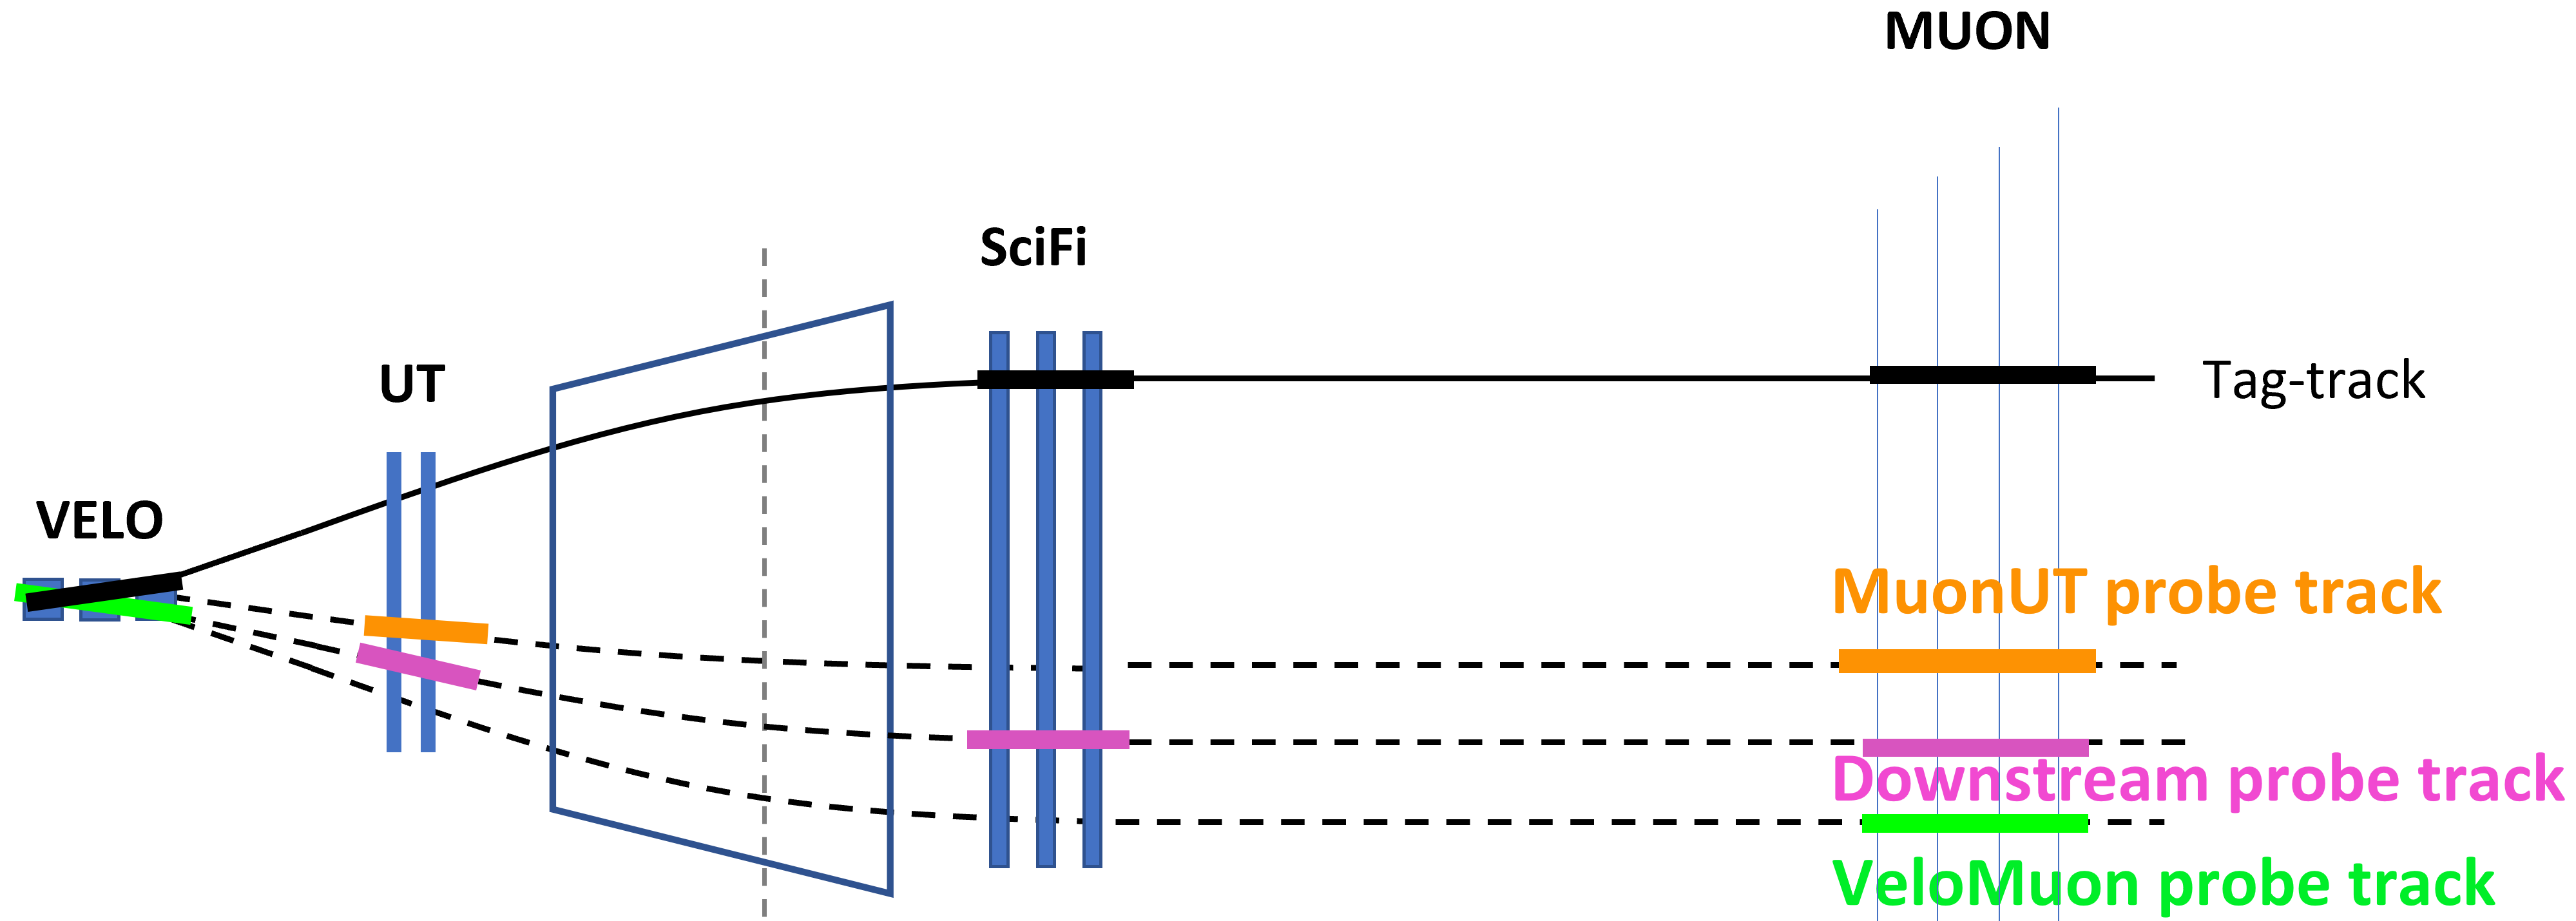
\includegraphics[width=0.75\textwidth]{Plots/Tag_and_probe_method.png}
    \caption*{\small Figure from \href{https://www.physi.uni-heidelberg.de/Publications/PhD_thesis.pdf}{Figure by Rowina}}
  \end{figure}
  \begin{itemize}
    \item{Fully reconstruct one muon from $J/\psi\to\mu^+\mu^-$}
    \item{Partially reconstruct the other muon}
    \item{Match hits in specific sub-detector with partially reconstructed track}
  \end{itemize}
  \begin{equation*}
    \epsilon_{\rm track} = \frac{N_{\rm matched}}{N_{\rm matched} + N_{\rm failed}}
  \end{equation*}
\end{frame}

\begin{frame}{Overlap criteria in matching}
  \vspace{0.0cm}
  {Matching is done by comparing the hits of the probe track with a long track in each subdetector}
  \vspace{0.2cm}
  \begin{center}
    \begin{tabular}{ccccc}
      \hline
      Method     & Velo     & UT              & SciFi    & Muon \\
      \hline
      VeloMuon   & $> 40\%$ & --              & --       & $> 40\%$ \\
      Downstream & --       & --              & $> 40\%$ & $> 40\%$ \\
      MuonUT     & --       & $0$ or $> 40\%$ & --       & $> 40\%$ \\
      \hline
    \end{tabular}
  \end{center}
  {Note:}
  \begin{itemize}
    \item{Matching was originally performed in a trigger line}
    \item{We now have functors for direct access to overlap fractions}
    \item{Requires rerunning reconstruction in 2024, as long-track information was not persisted}
  \end{itemize}
\end{frame}

\begin{frame}{Overview of previous work}
  \vspace{0.0cm}
  {What I'm showing today is based on Rowina's thesis work}
  \vspace{0.2cm}
  \begin{itemize}
    \setlength\itemsep{0.8em}
    \item{Previous presentation \href{https://indico.cern.ch/event/1577588/\#6-status-tracking-efficiencies}{here}}
    \item{Rowina's thesis \href{https://repository.cern/records/n2g9v-81z15}{here}}
  \end{itemize}
  \vspace{0.5cm}
  {Today's results are from TrackCalib2, which was maintained by Maurice}
  \vspace{0.2cm}
  \begin{itemize}
    \setlength\itemsep{0.8em}
    \item{Fitter independent from Rowina's code, but results are consistent}
    \item{Tuples are currently fetched directly from an AP}
  \end{itemize}
\end{frame}

\begin{frame}{Tracking efficiency plan}
  \vspace{0.0cm}
  {\Large What are we providing analysts?}
  \vspace{0.2cm}
  \begin{enumerate}
    \setlength\itemsep{1.0em}
    \item{Table of Velo and SciFi tracking efficiencies}
    \begin{itemize}
      \setlength\itemsep{0.3em}
      \item[-]{Measured with a tag-and-probe method}
      \item[-]{Both MC and data}
      \item[-]{Provided in 1D $p$ and $\eta$ bins, and also 2D $p$--$\eta$ bins}
      \item[-]{Plan to provide charge integrated numbers, and also $\mu^+$ and $\mu^-$ separately}
    \end{itemize}
    \item{Data/MC long track efficiency ratio}
    \begin{itemize}
      \setlength\itemsep{0.3em}
      \item[-]{Long track efficiency from product of Velo and SciFi efficiencies}
      \item[-]{2D $p$--$\eta$ binning MC reweighting in physics analysis}
      \item[-]{Statistical uncertainties from limited data/MC sample sizes}
      \item[-]{Dominant systematic uncertainty from MuonUT-Combined difference}
    \end{itemize}
  \end{enumerate}
\end{frame}

\begin{frame}{Overview of current progress}
  \vspace{0.0cm}
  {\large What I will talk about today on tracking efficiencies:}
  \vspace{0.2cm}
  \begin{enumerate}
    \setlength\itemsep{1.0em}
    \item{Block 1a vs 1b studies}
    \item{Results for tracking efficiencies (2024 blocks 2, 1a, 5--8, $pp$ ref, 2025 pre-TS)}
    \item{Guide to TrackCalib2}
  \end{enumerate}
\end{frame}

\begin{frame}{Overview of current progress}
  \vspace{0.0cm}
  {\large What I will talk about today on tracking efficiencies:}
  \vspace{0.2cm}
  \begin{enumerate}
    \setlength\itemsep{1.0em}
    \item{\textbf{Block 1a vs 1b studies}}
    \item{2024 tracking efficiencies (blocks 2, 1a, 5--8, $pp$ ref)}
    \item{2025 tracking efficiencies (pre-TS)}
    \item{Guide to TrackCalib2}
  \end{enumerate}
\end{frame}

\begin{frame}{Block 1a vs 1b}
  \vspace{0.0cm}
  {\large Block 1a (fills 9982--10012, top) vs 1b (fills 10017--10056, bottom)}
  \begin{figure}[htb]
    \centering
    \begin{subfigure}{0.5\textwidth}
      \centering
      
\includegraphics[width=0.75\textwidth]{Plots/trackeff_Data_VeloMuon_ETA_2024_Block1a_samples.pdf}
    \end{subfigure}%
    \begin{subfigure}{0.5\textwidth}
      \centering
      
\includegraphics[width=0.75\textwidth]{Plots/trackeff_MC_VeloMuon_ETA_2024_Block1a_samples.pdf}
    \end{subfigure}
    \begin{subfigure}{0.5\textwidth}
      \centering
      
\includegraphics[width=0.75\textwidth]{Plots/trackeff_Data_VeloMuon_ETA_2024_Block1b_samples.pdf}
    \end{subfigure}%
    \begin{subfigure}{0.5\textwidth}
      \centering
      
\includegraphics[width=0.75\textwidth]{Plots/trackeff_MC_VeloMuon_ETA_2024_Block1b_samples.pdf}
    \end{subfigure}
  \end{figure}
  {SciFi T2L0Q0M1H0 FE was excluded on 17th August}
\end{frame}

\begin{frame}{Block 1a vs 1b}
  \vspace{0.0cm}
  {\large MC doesn't seem to describe the drop in tracking efficiency well...}
  \vspace{0.2cm}
  \begin{itemize}
    \setlength\itemsep{1.5em}
    \item{We will check with Simulation people}
    \item{Note: The ``hole'' in the SciFi is only visible when looking at tracks in the 3rd quadrant, the integrated numbers show negligible differences between block 1a and block 1b}
    \item{We propose that all tracking efficiencies are only provided for block 1a}
    \item{Analyses that are sensitive to this missing SciFi FE should exclude block 1b, other analyses can use results for block 1a as a proxy for block 1b}
  \end{itemize}
\end{frame}

\begin{frame}{Overview of current progress}
  \vspace{0.0cm}
  {\large What I will talk about today on tracking efficiencies:}
  \vspace{0.2cm}
  \begin{enumerate}
    \setlength\itemsep{1.0em}
    \item{Block 1a vs 1b studies}
    \item{\textbf{2024 tracking efficiencies (blocks 2, 1a, 5--8, $\mathbf{pp}$ ref)}}
    \item{2025 tracking efficiencies (pre-TS)}
    \item{Guide to TrackCalib2}
  \end{enumerate}
\end{frame}

\begin{frame}{Remarks on current results}
  \vspace{0.0cm}
  {\large Remark on resprucing of 24c4:}
  \vspace{0.2cm}
  \begin{itemize}
    \setlength\itemsep{1.0em}
    \item{$40\%$ prescale present in sprucing}
    \item{Very limited statistics, especially in MuonUT}
    \item{Turcal resprucing campaign (24r1) started 3 weeks ago...}
    \item{... but a bug in the merging step delayed the campaign until last week}
    \item{Results shown for 24c4, to be updated with 24r1 in a few weeks}
  \end{itemize}
\end{frame}

\begin{frame}{Remarks on current results}
  \vspace{0.0cm}
  {\large Remark on phase-space differences between 2024 and 2025:}
  \vspace{0.2cm}
  \begin{itemize}
    \setlength\itemsep{1.0em}
    \item{Probe muon $p_T$ cut was at $500$~MeV in 2024}
    \item{Loosened to $100$~MeV in 2025}
    \item{Therefore cannot compare 2024 and 2025 directly}
  \end{itemize}
\end{frame}

\begin{frame}{Efficiency comparisons}
  \vspace{0.0cm}
  {\large Comparison of tracking efficiencies in all data blocks}
  \begin{figure}[htb]
    \centering
    \begin{subfigure}{0.5\textwidth}
      \centering
      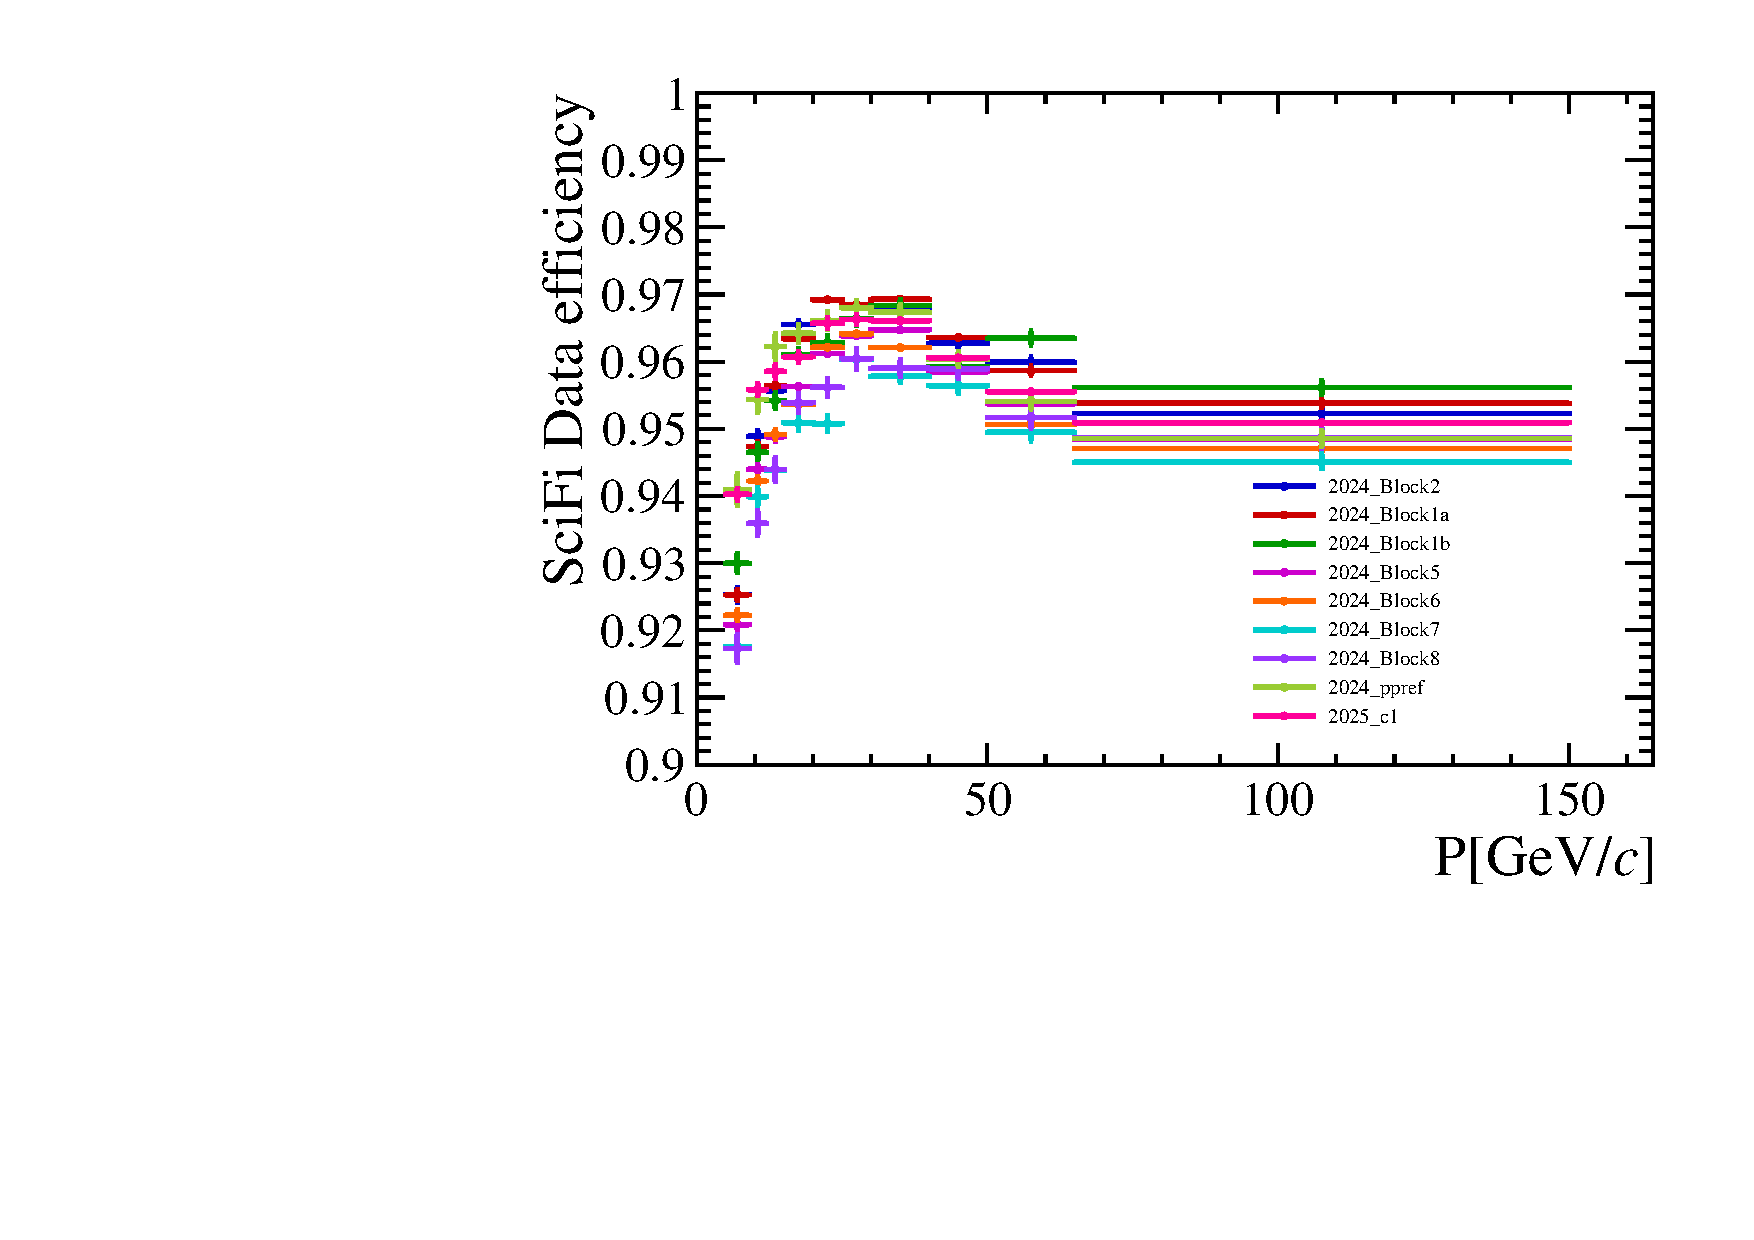
\includegraphics[width=0.75\textwidth]{Plots/trackeff_Data_VeloMuon_P_default_samples.pdf}
    \end{subfigure}%
    \begin{subfigure}{0.5\textwidth}
      \centering
      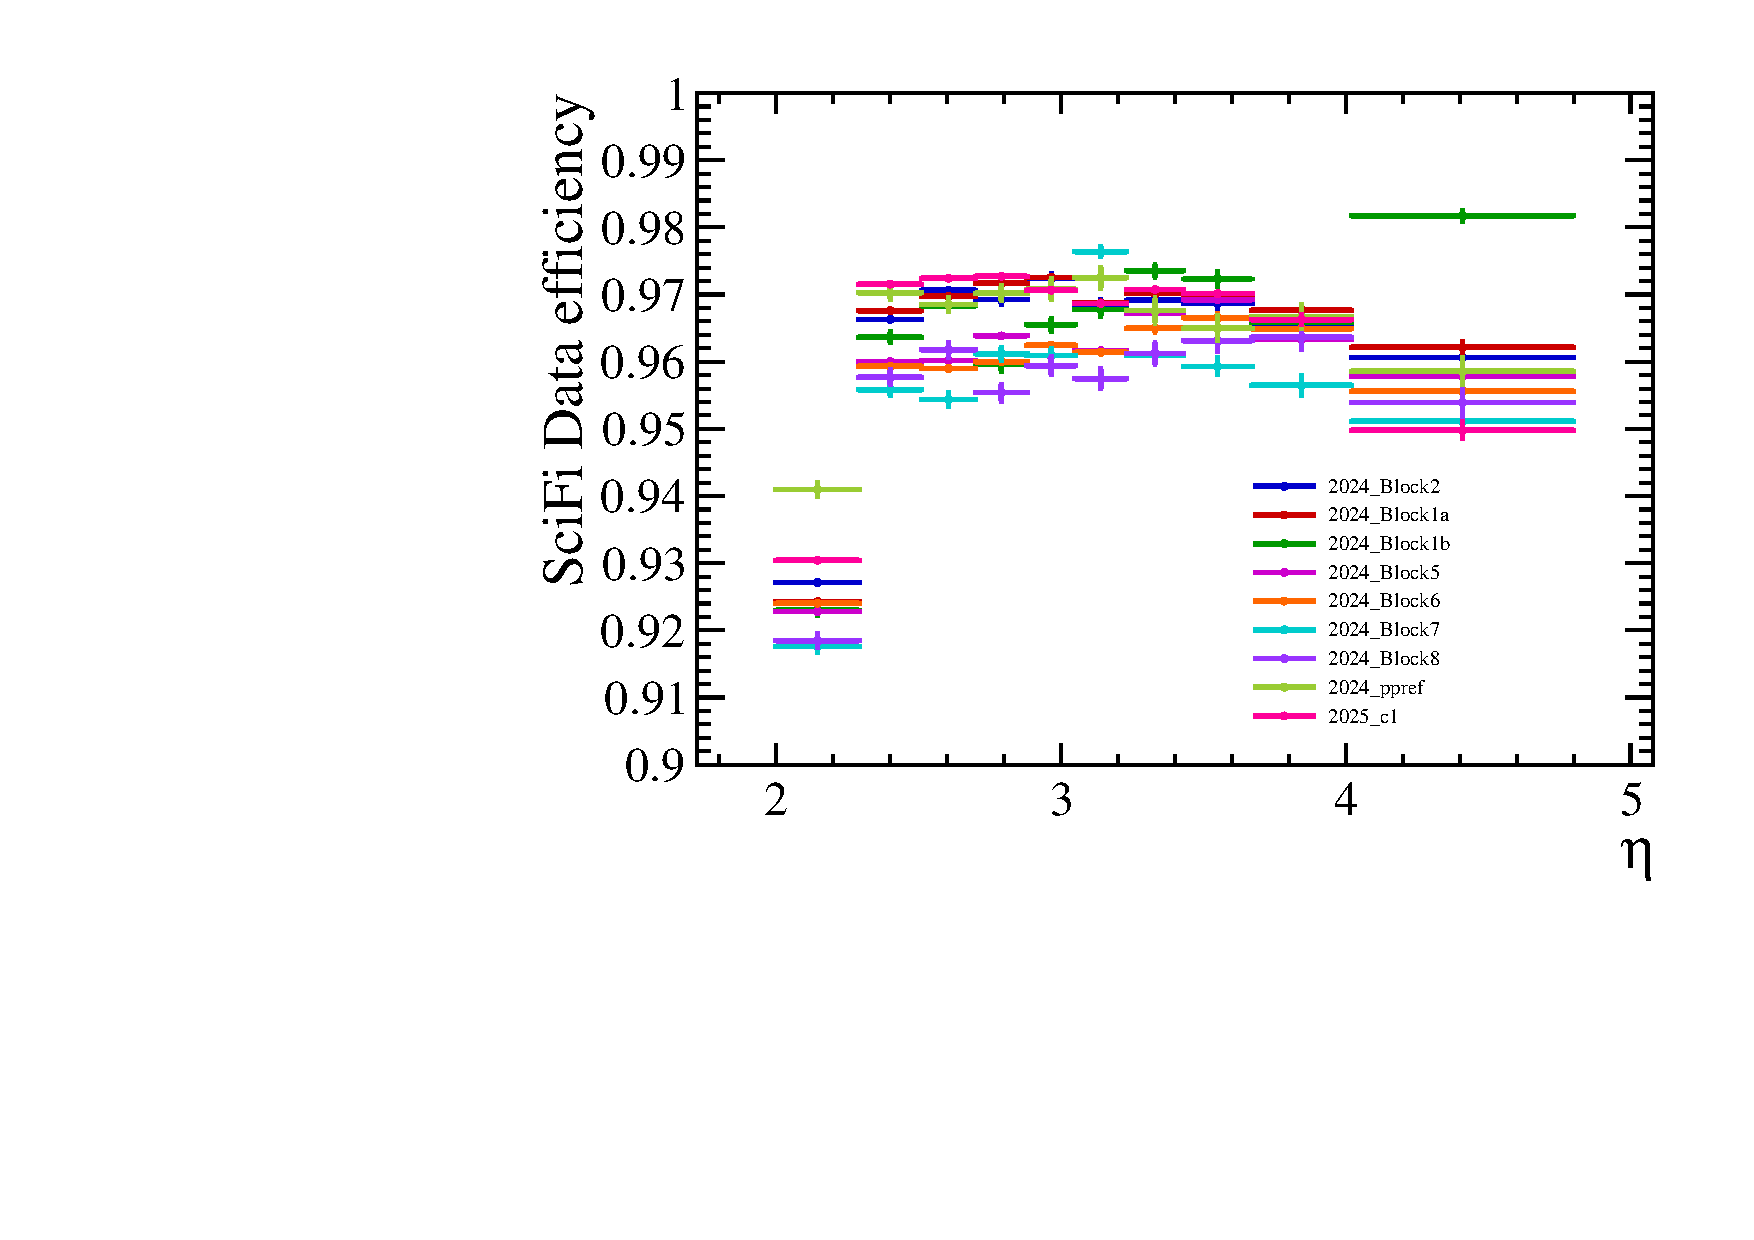
\includegraphics[width=0.75\textwidth]{Plots/trackeff_Data_VeloMuon_ETA_default_samples.pdf}
    \end{subfigure}
    \begin{subfigure}{0.5\textwidth}
      \centering
      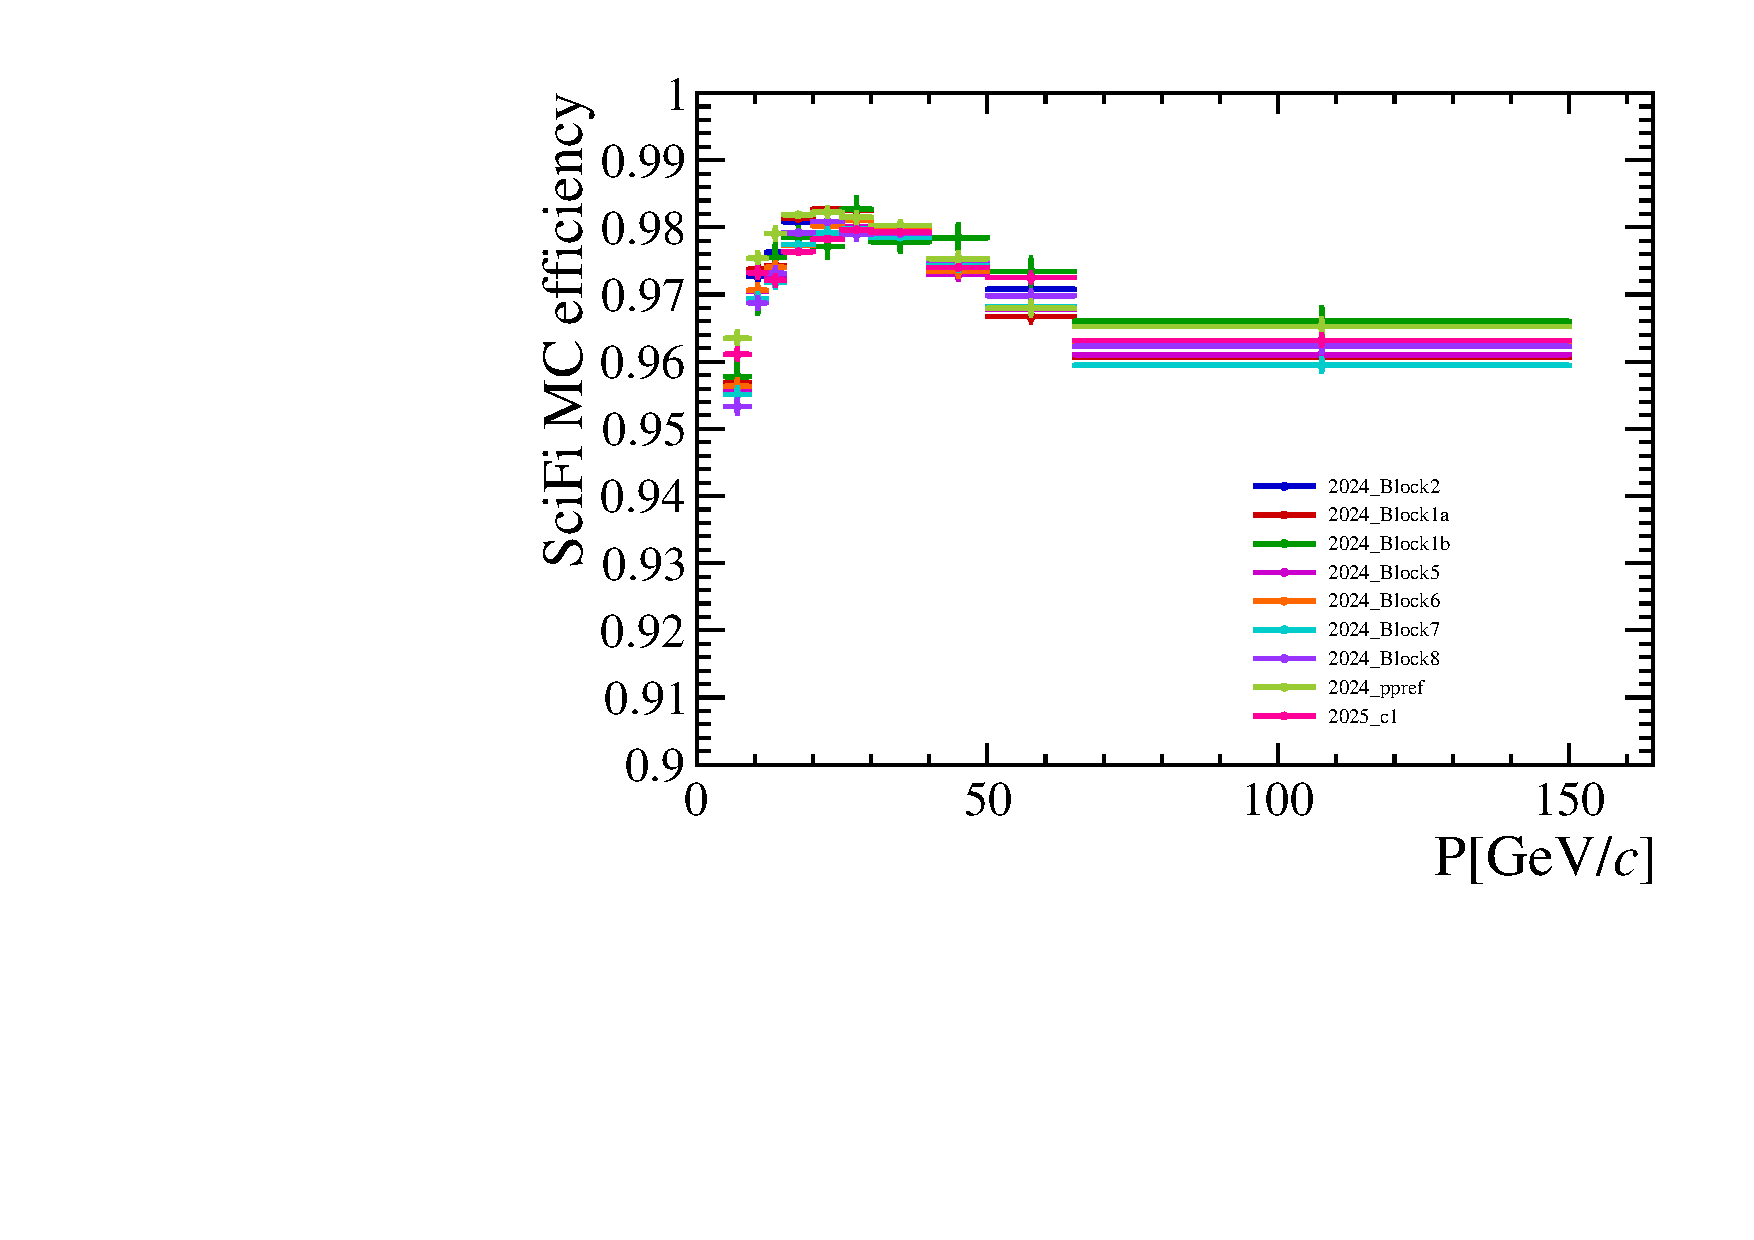
\includegraphics[width=0.75\textwidth]{Plots/trackeff_MC_VeloMuon_P_default_samples.pdf}
    \end{subfigure}%
    \begin{subfigure}{0.5\textwidth}
      \centering
      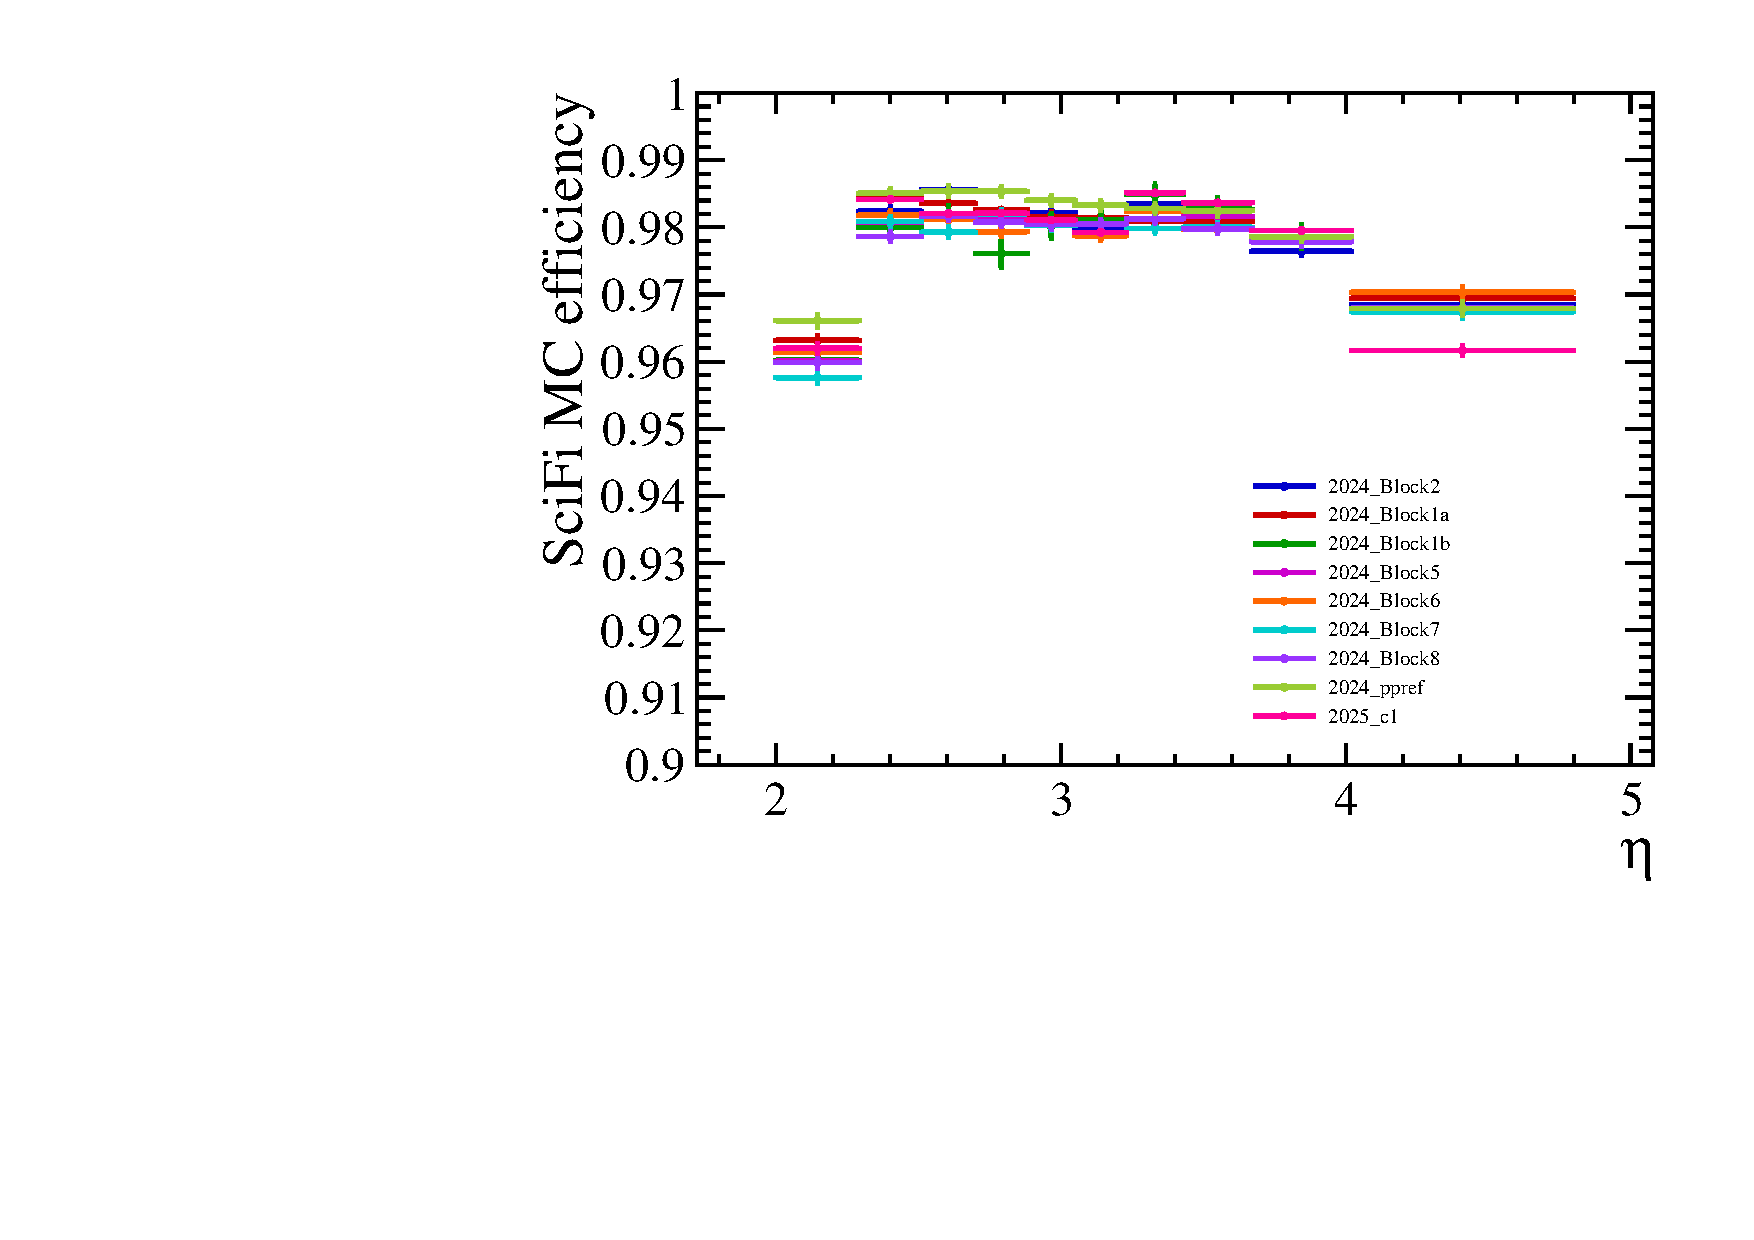
\includegraphics[width=0.75\textwidth]{Plots/trackeff_MC_VeloMuon_ETA_default_samples.pdf}
    \end{subfigure}
  \end{figure}
  \vspace{-0.4cm}
  {SciFi efficiencies}
\end{frame}

\begin{frame}{Efficiency comparisons}
  \vspace{0.0cm}
  {\large Comparison of tracking efficiencies in all data blocks}
  \begin{figure}[htb]
    \centering
    \begin{subfigure}{0.5\textwidth}
      \centering
      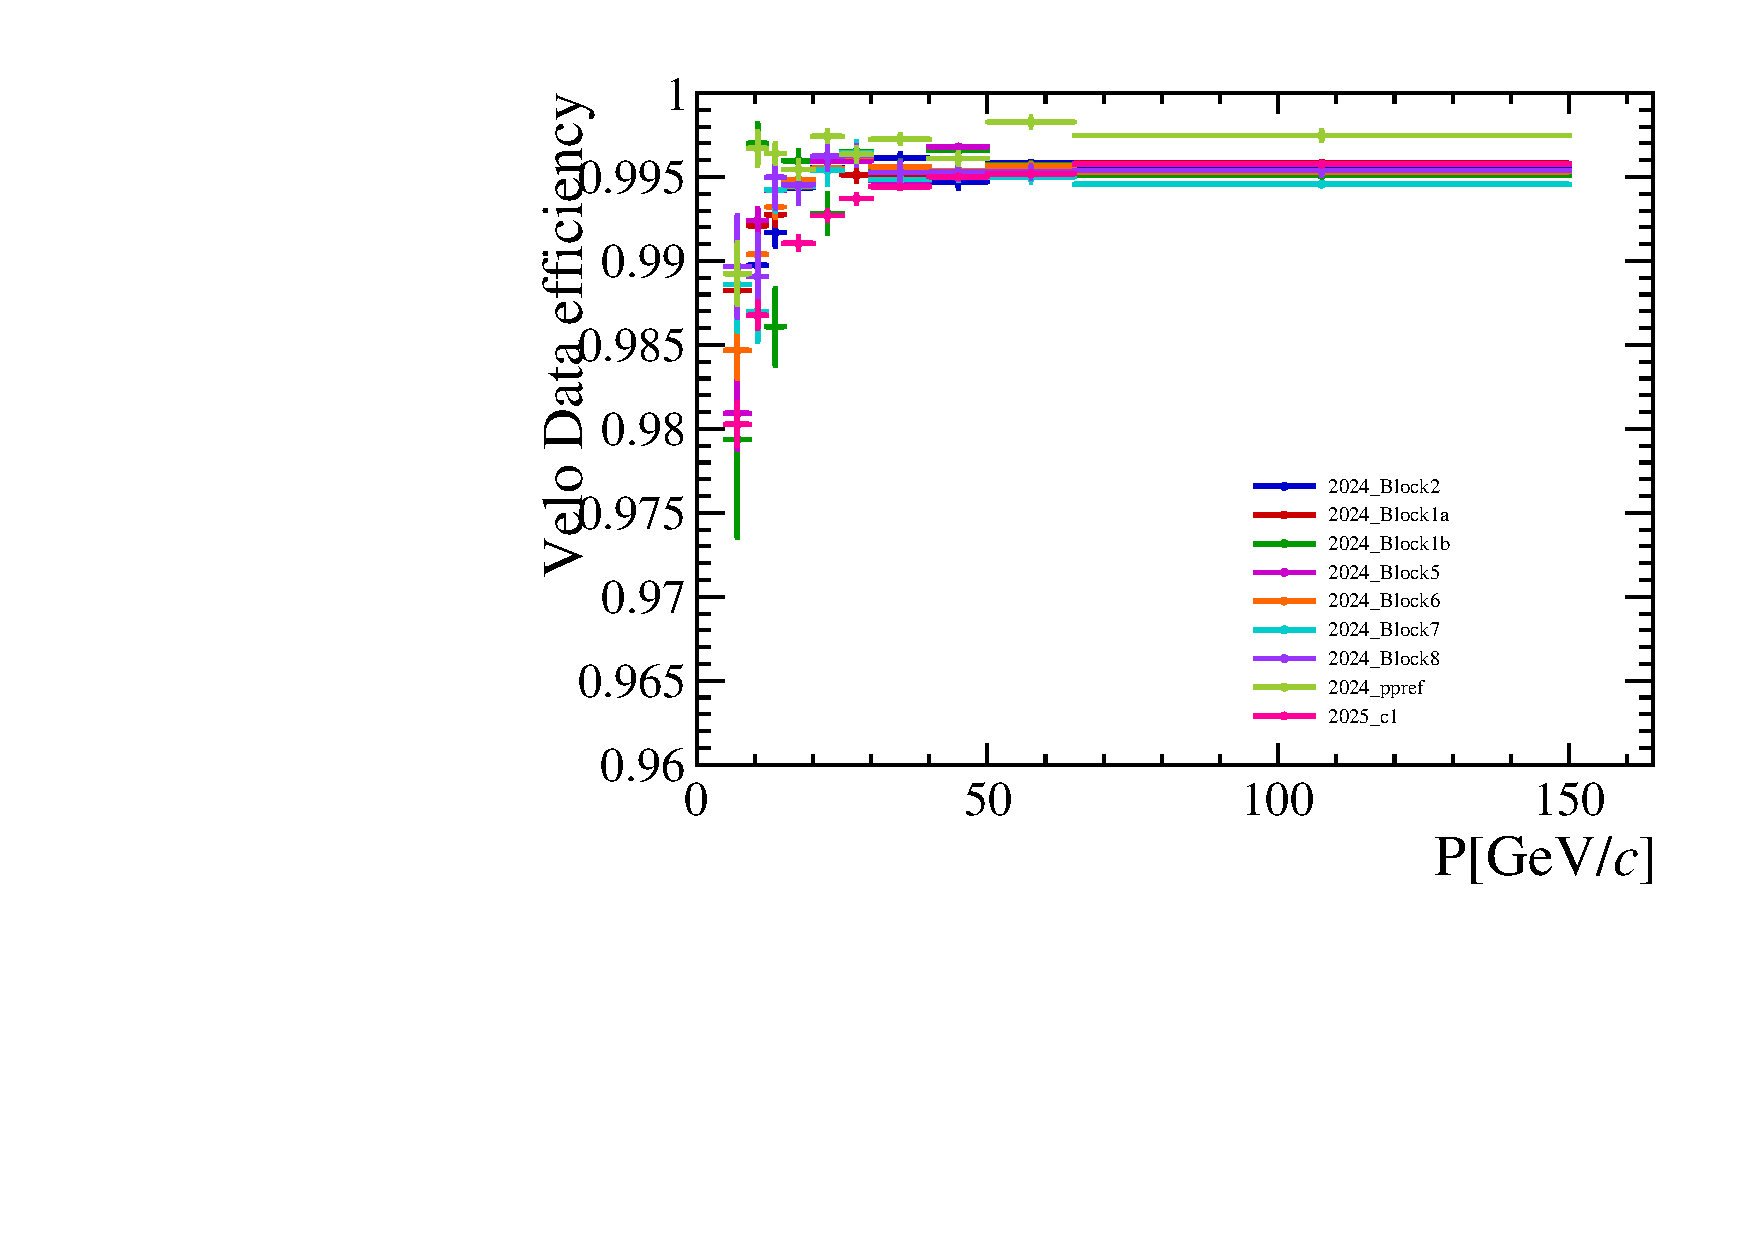
\includegraphics[width=0.75\textwidth]{Plots/trackeff_Data_Downstream_P_default_samples.pdf}
    \end{subfigure}%
    \begin{subfigure}{0.5\textwidth}
      \centering
      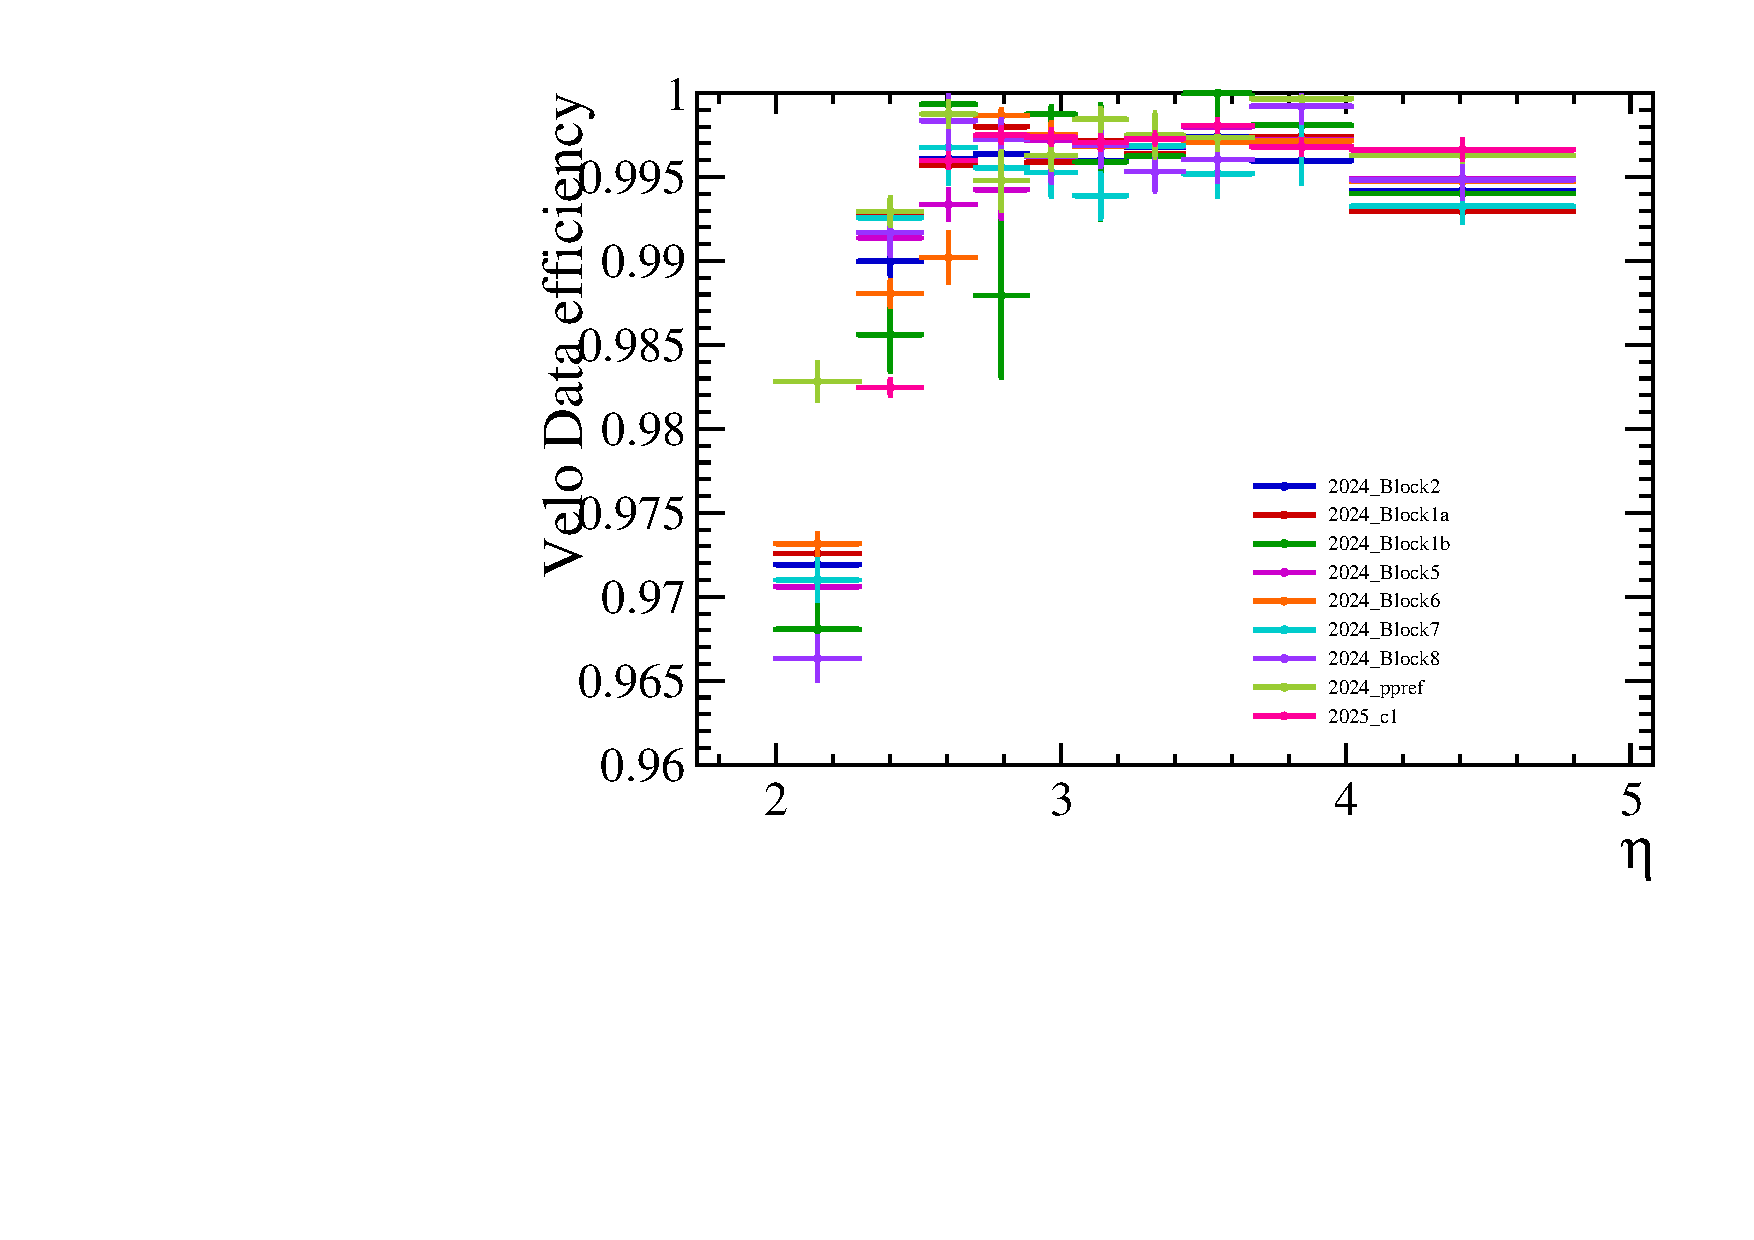
\includegraphics[width=0.75\textwidth]{Plots/trackeff_Data_Downstream_ETA_default_samples.pdf}
    \end{subfigure}
    \begin{subfigure}{0.5\textwidth}
      \centering
      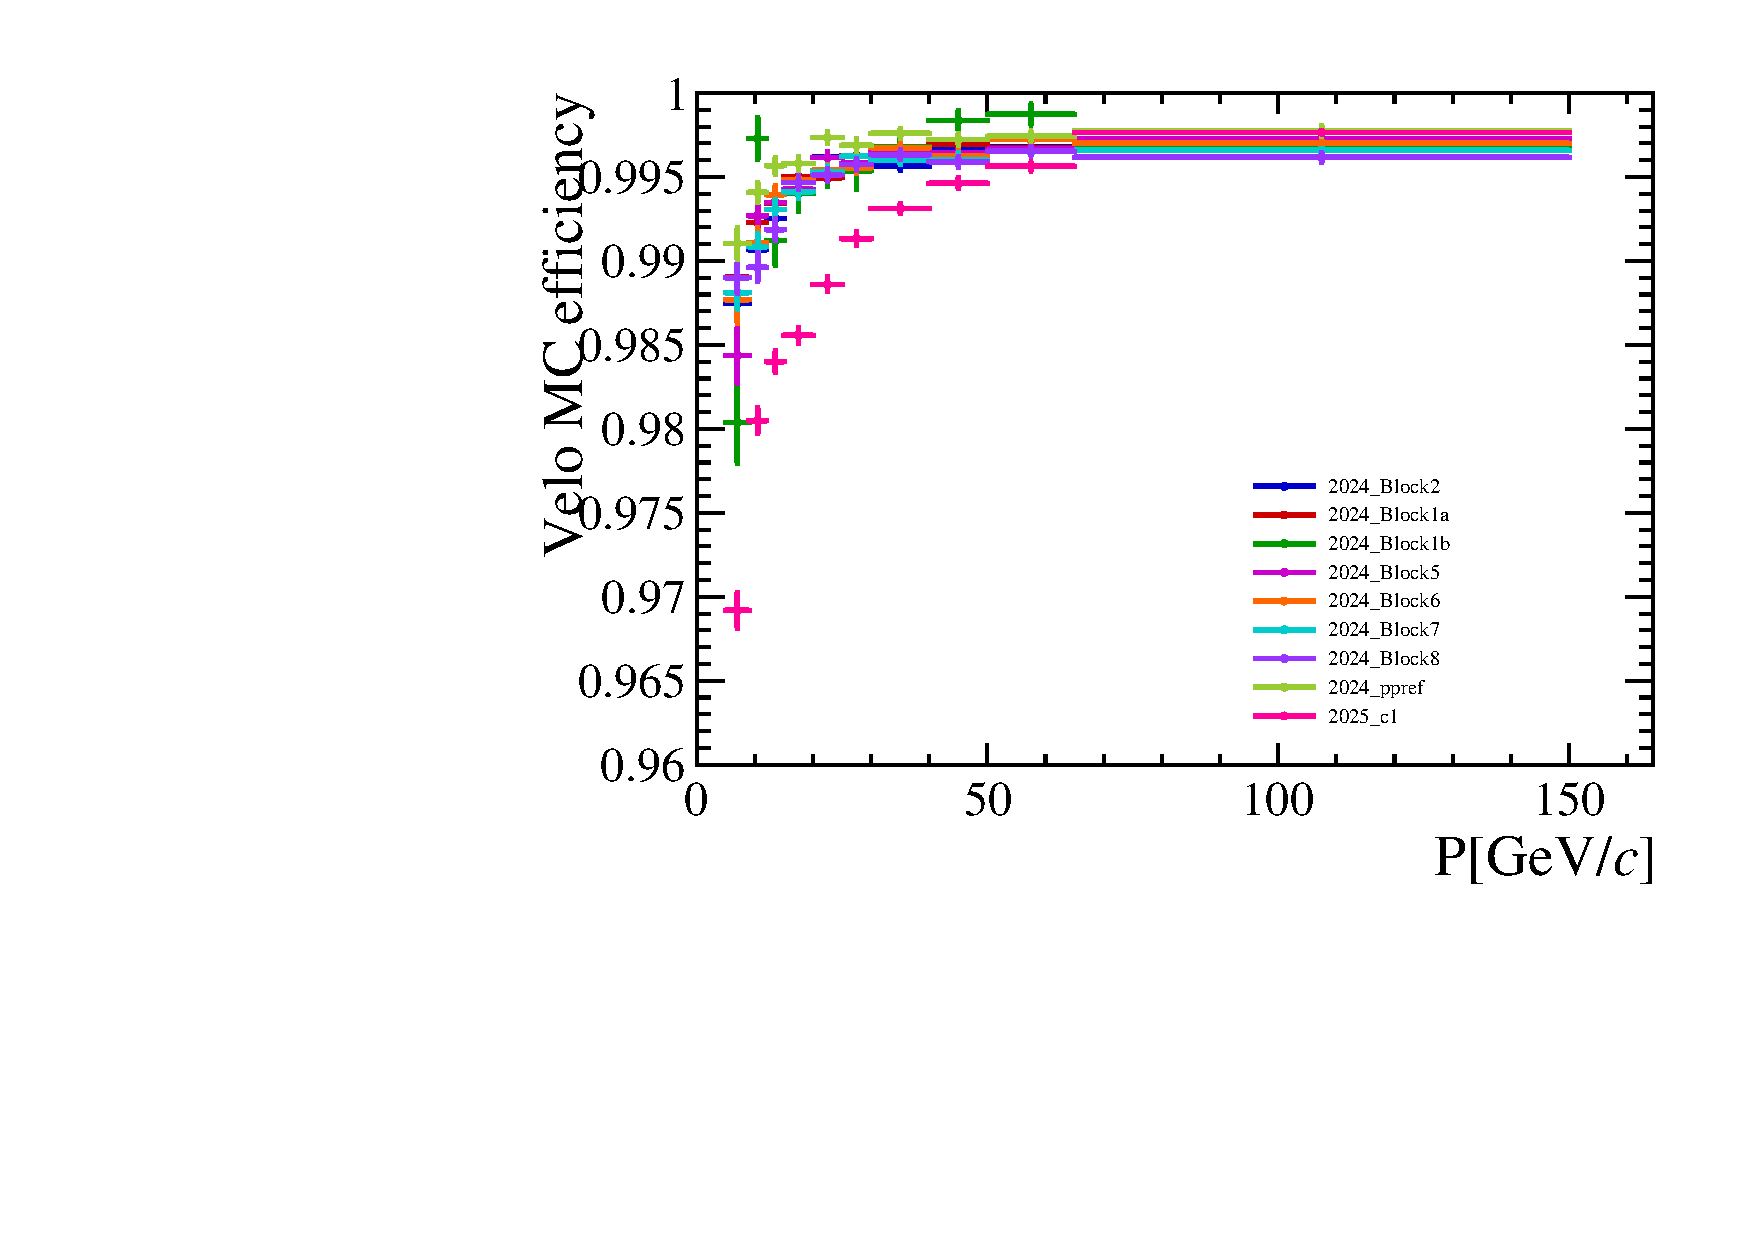
\includegraphics[width=0.75\textwidth]{Plots/trackeff_MC_Downstream_P_default_samples.pdf}
    \end{subfigure}%
    \begin{subfigure}{0.5\textwidth}
      \centering
      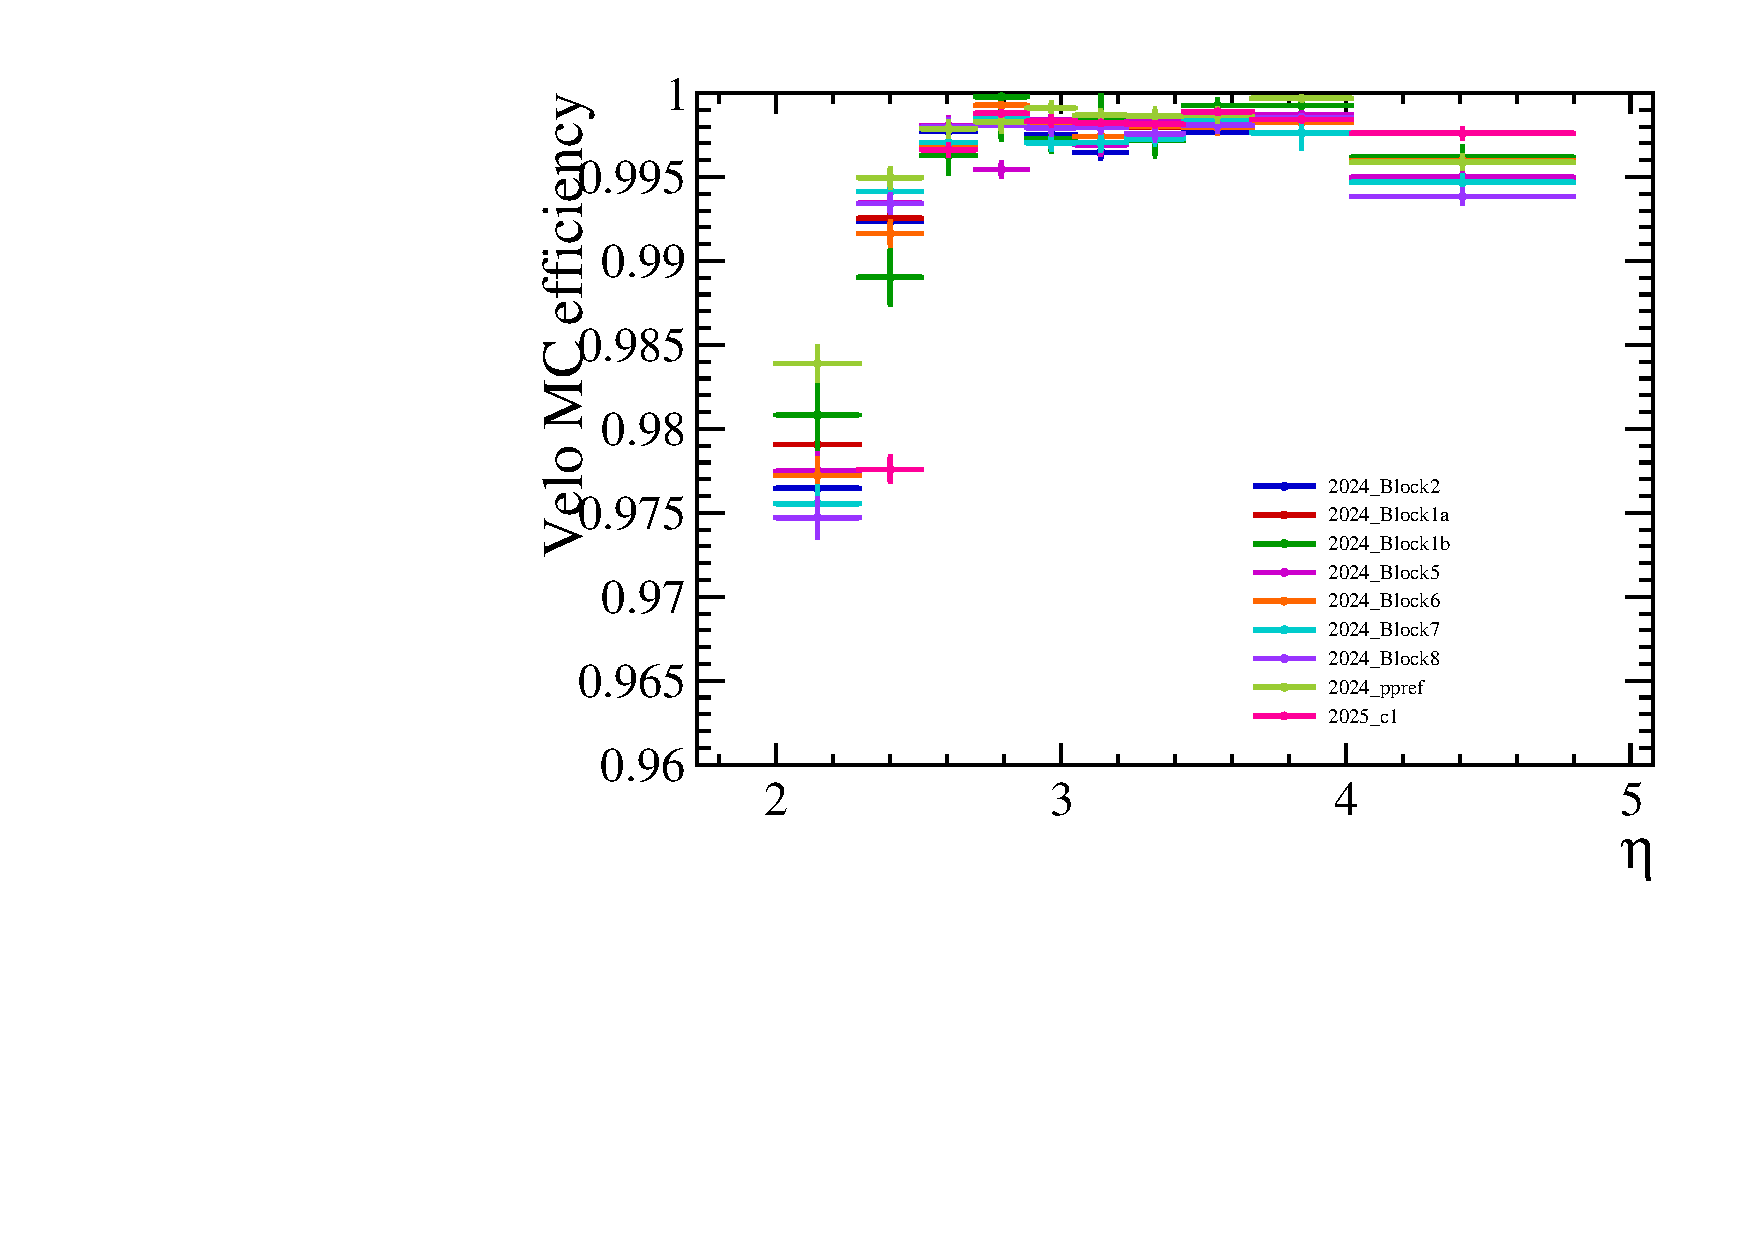
\includegraphics[width=0.75\textwidth]{Plots/trackeff_MC_Downstream_ETA_default_samples.pdf}
    \end{subfigure}
  \end{figure}
  \vspace{-0.4cm}
  {Velo efficiencies}
\end{frame}

\begin{frame}{Efficiency comparisons}
  \vspace{0.0cm}
  {\large Comparison of tracking efficiencies in all data blocks}
  \begin{figure}[htb]
    \centering
    \begin{subfigure}{0.5\textwidth}
      \centering
      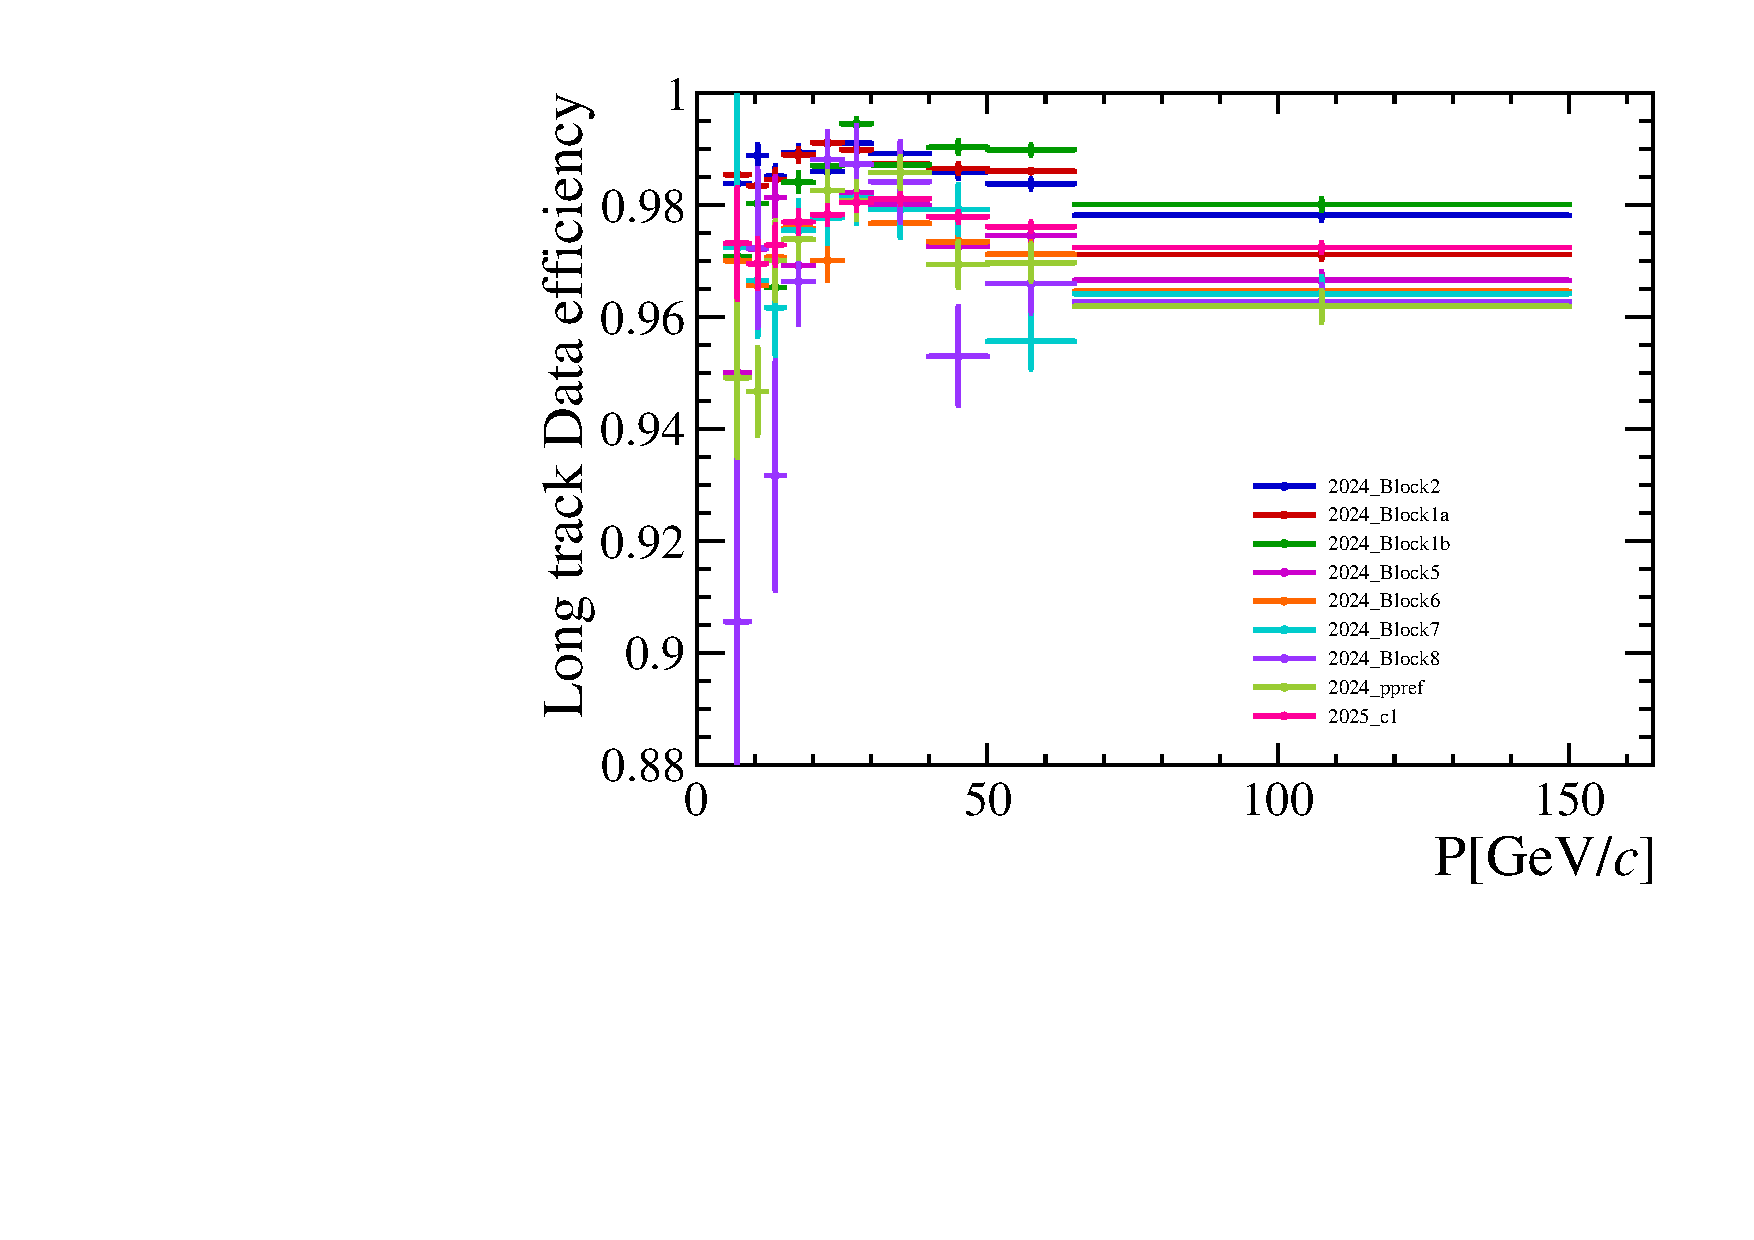
\includegraphics[width=0.75\textwidth]{Plots/trackeff_Data_MuonUT_P_default_samples.pdf}
    \end{subfigure}%
    \begin{subfigure}{0.5\textwidth}
      \centering
      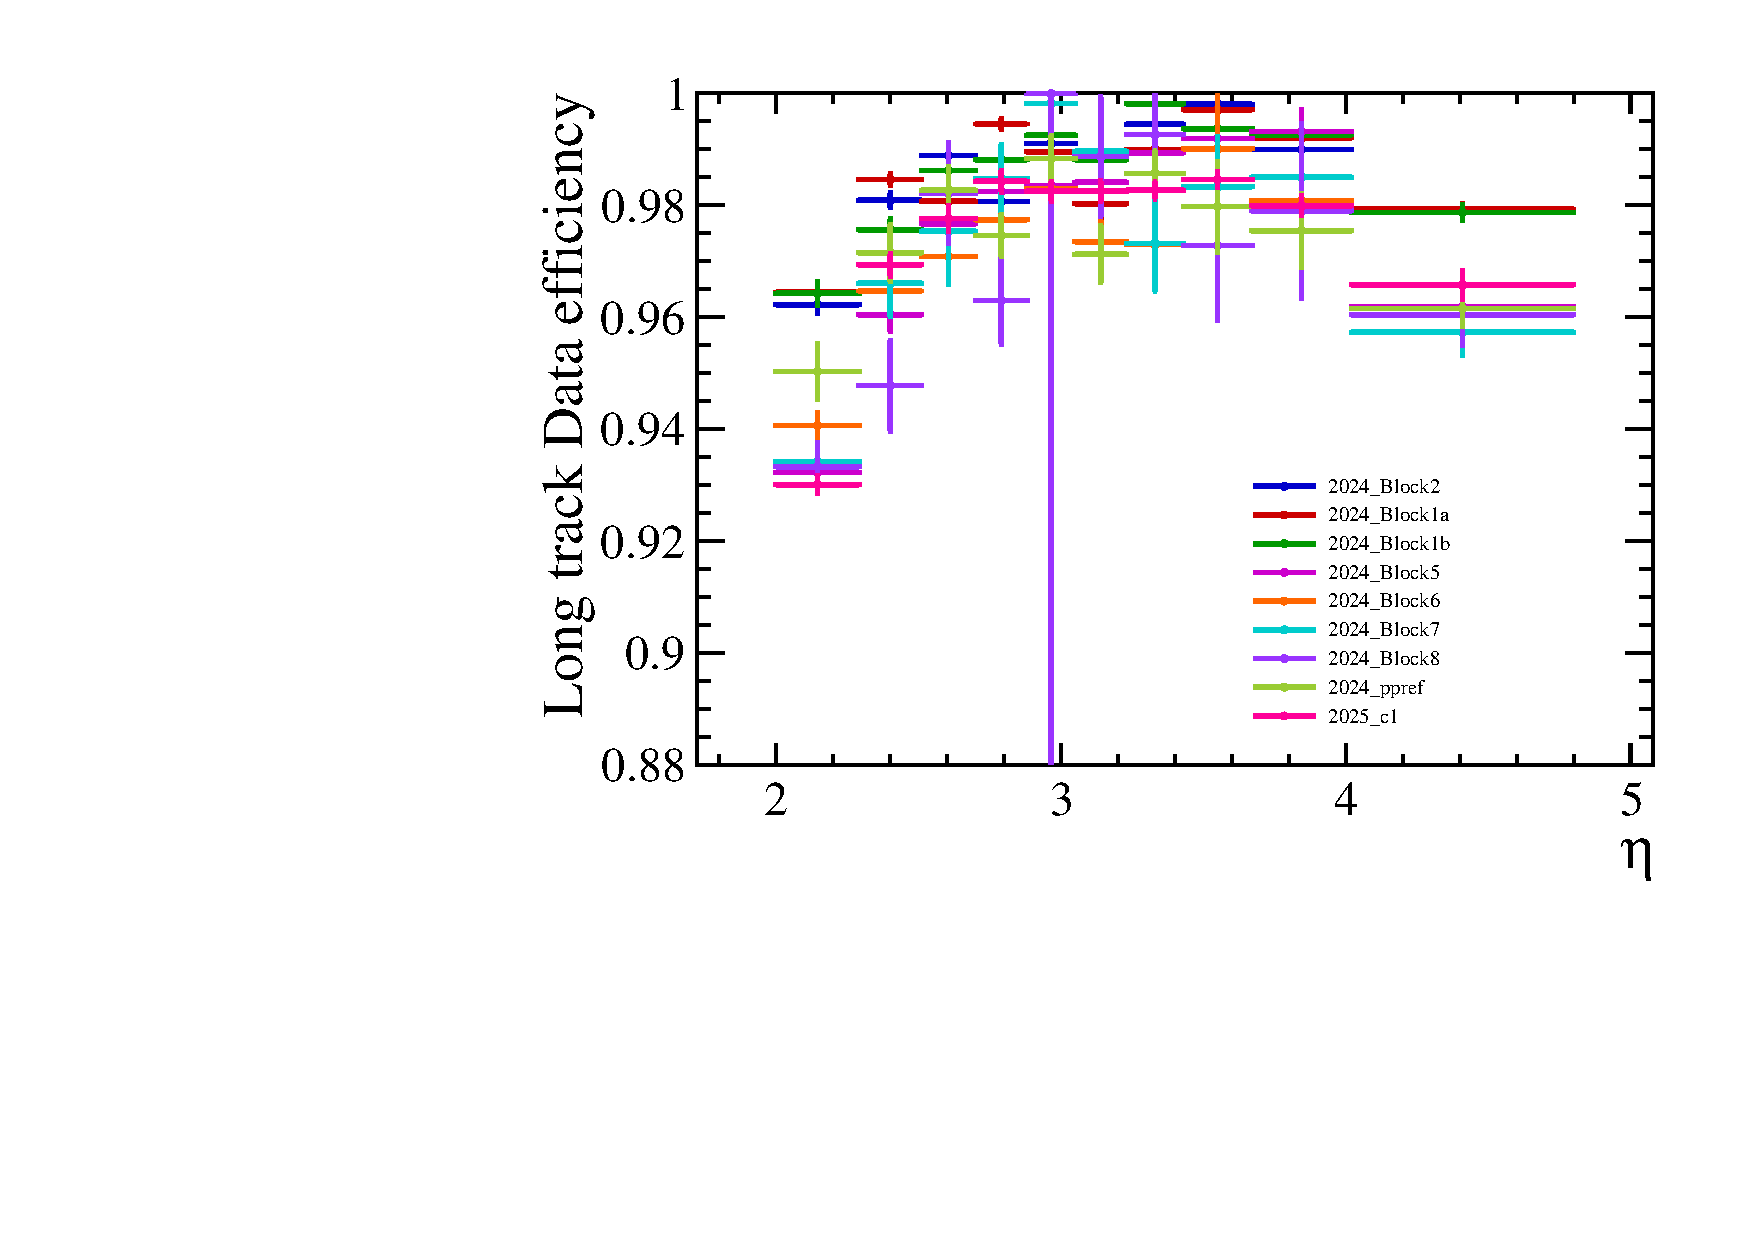
\includegraphics[width=0.75\textwidth]{Plots/trackeff_Data_MuonUT_ETA_default_samples.pdf}
    \end{subfigure}
    \begin{subfigure}{0.5\textwidth}
      \centering
      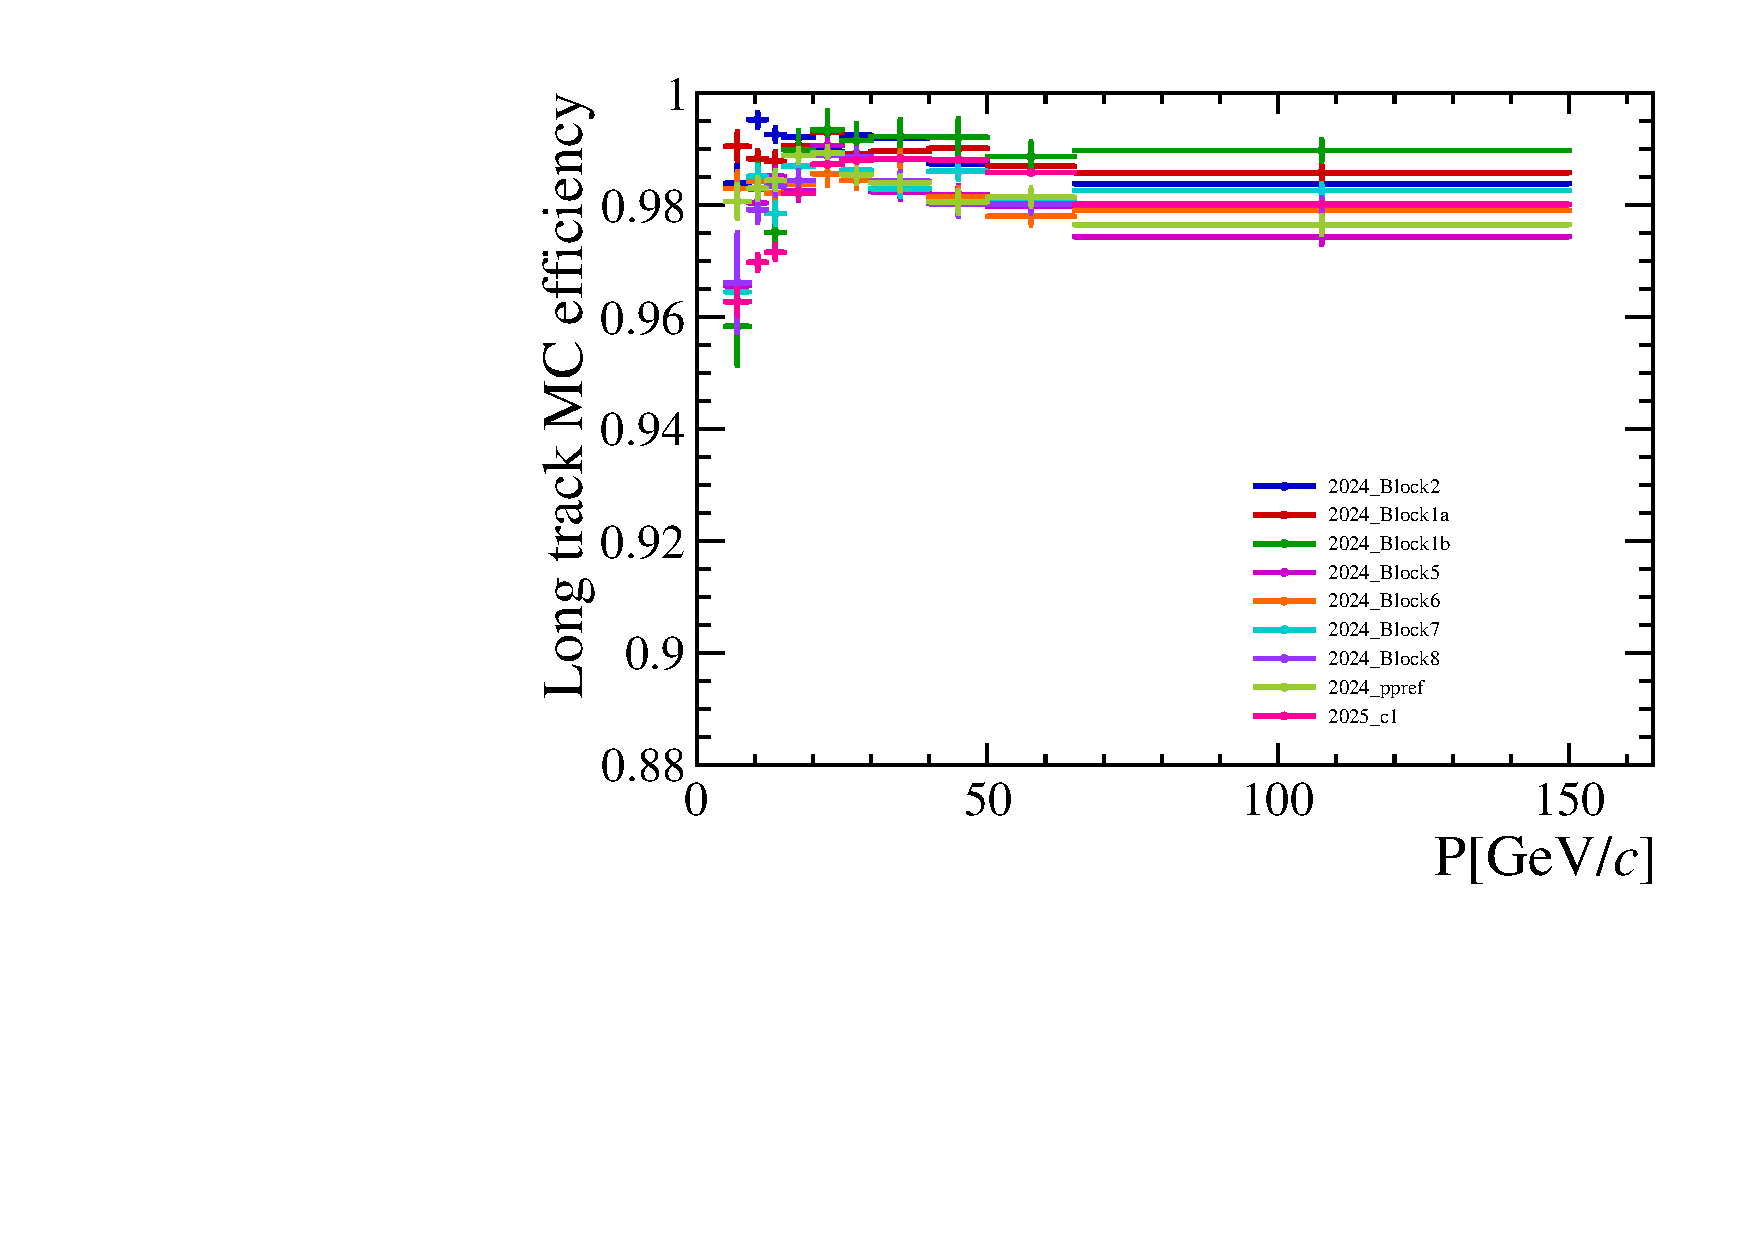
\includegraphics[width=0.75\textwidth]{Plots/trackeff_MC_MuonUT_P_default_samples.pdf}
    \end{subfigure}%
    \begin{subfigure}{0.5\textwidth}
      \centering
      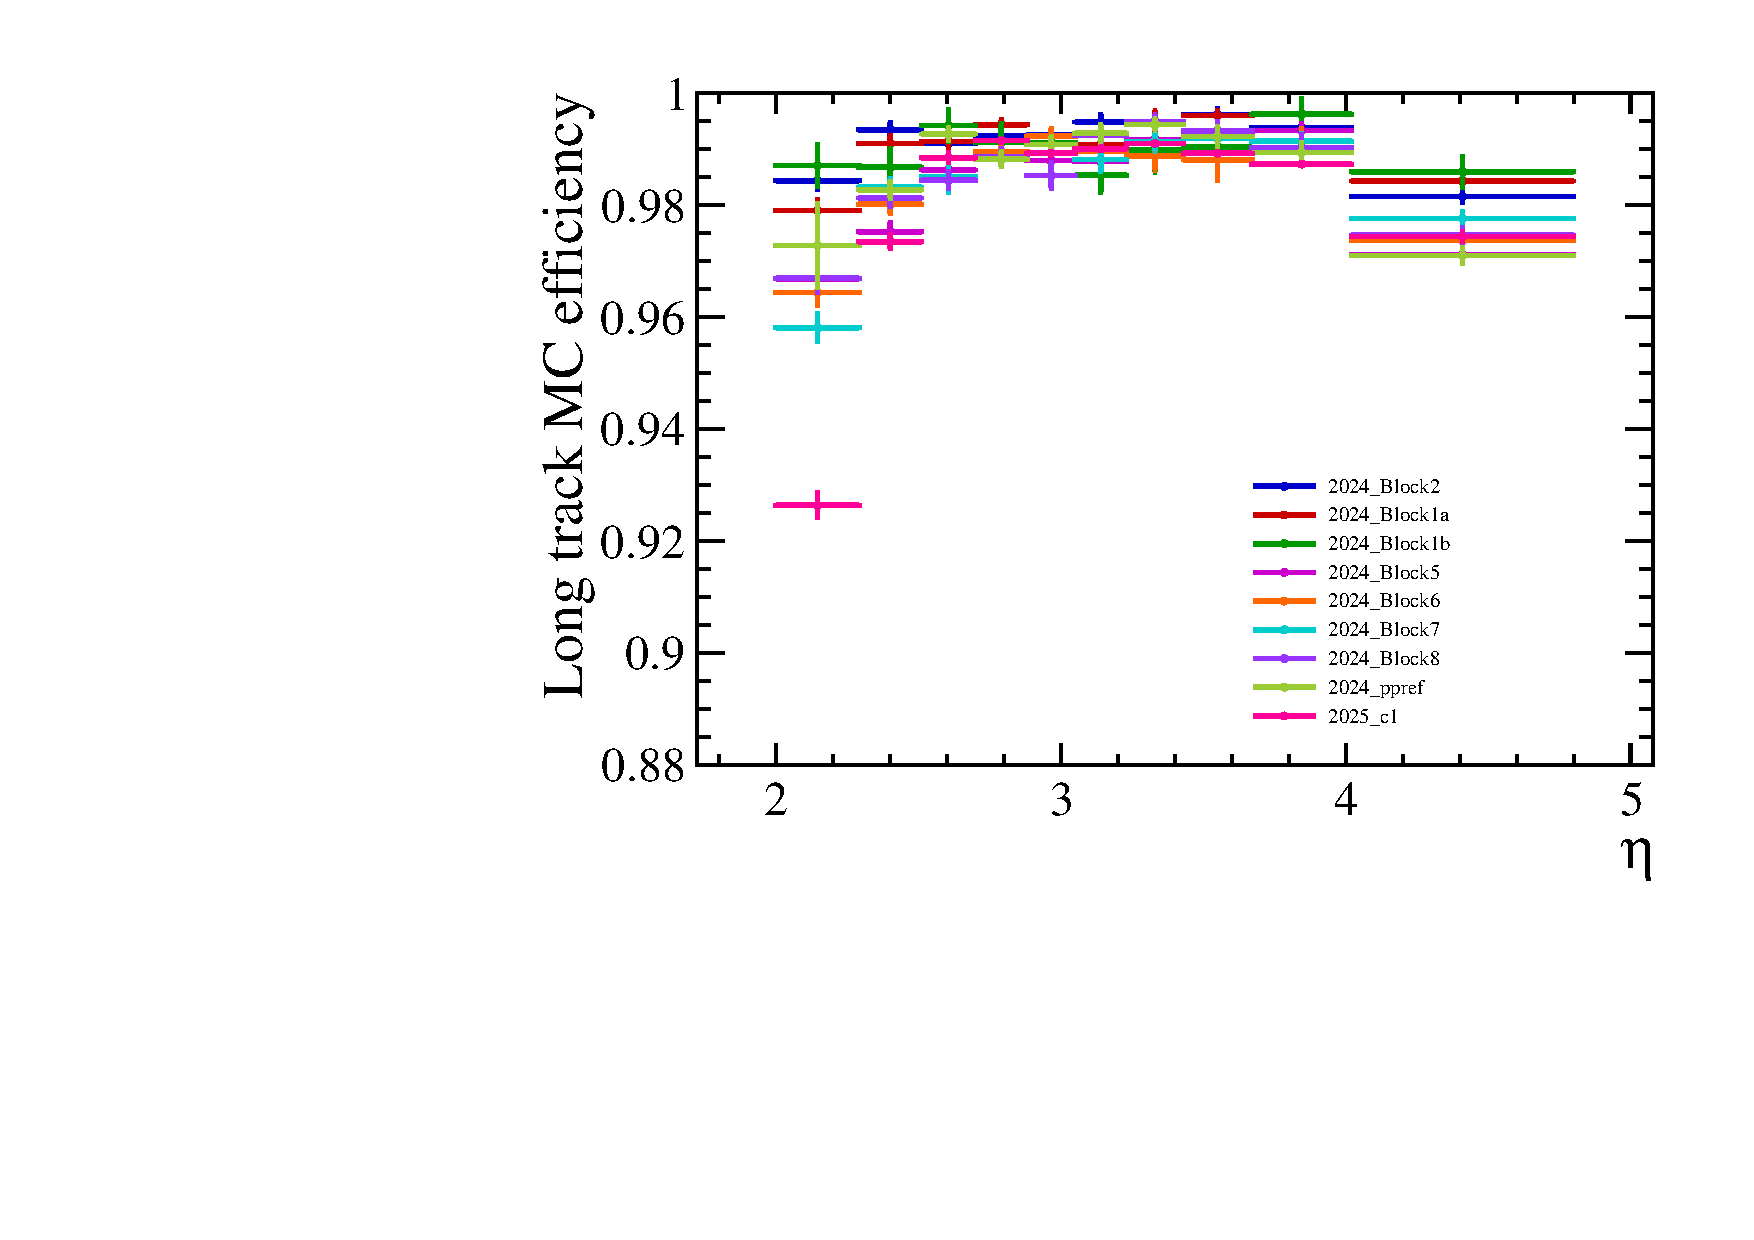
\includegraphics[width=0.75\textwidth]{Plots/trackeff_MC_MuonUT_ETA_default_samples.pdf}
    \end{subfigure}
  \end{figure}
  \vspace{-0.4cm}
  {Long track efficiencies}
\end{frame}

\begin{frame}{General observations}
  \vspace{0.0cm}
  {\large General observations on tracking efficiencies:}
  \vspace{0.2cm}
  \begin{enumerate}
    \setlength\itemsep{1.0em}
    \item{All data sets show consistent trends}
    \item{Performance seems to (slowly) drop over time}
  \end{enumerate}
  \vspace{0.4cm}
  {\large This is very encouraging! Several issues resolved, including:}
  \vspace{0.2cm}
  \begin{enumerate}
    \setlength\itemsep{1.0em}
    \item{Unusually high efficiencies in blocks 7/8}
    \item{Missing binds when rerunning reconstruction}
    \item{Large charge asymmetries in MuonUT samples}
  \end{enumerate}
  \vspace{0.2cm}
  {\large However, the low Velo efficiency in MC needs to be understood, so we will wait with the release of these numbers}
\end{frame}

\begin{frame}{Tracking efficiency data/MC ratio}
  \vspace{0.0cm}
  {\large Data/MC ratio}
  \begin{figure}[htb]
    \centering
    \begin{subfigure}{0.5\textwidth}
      \centering
      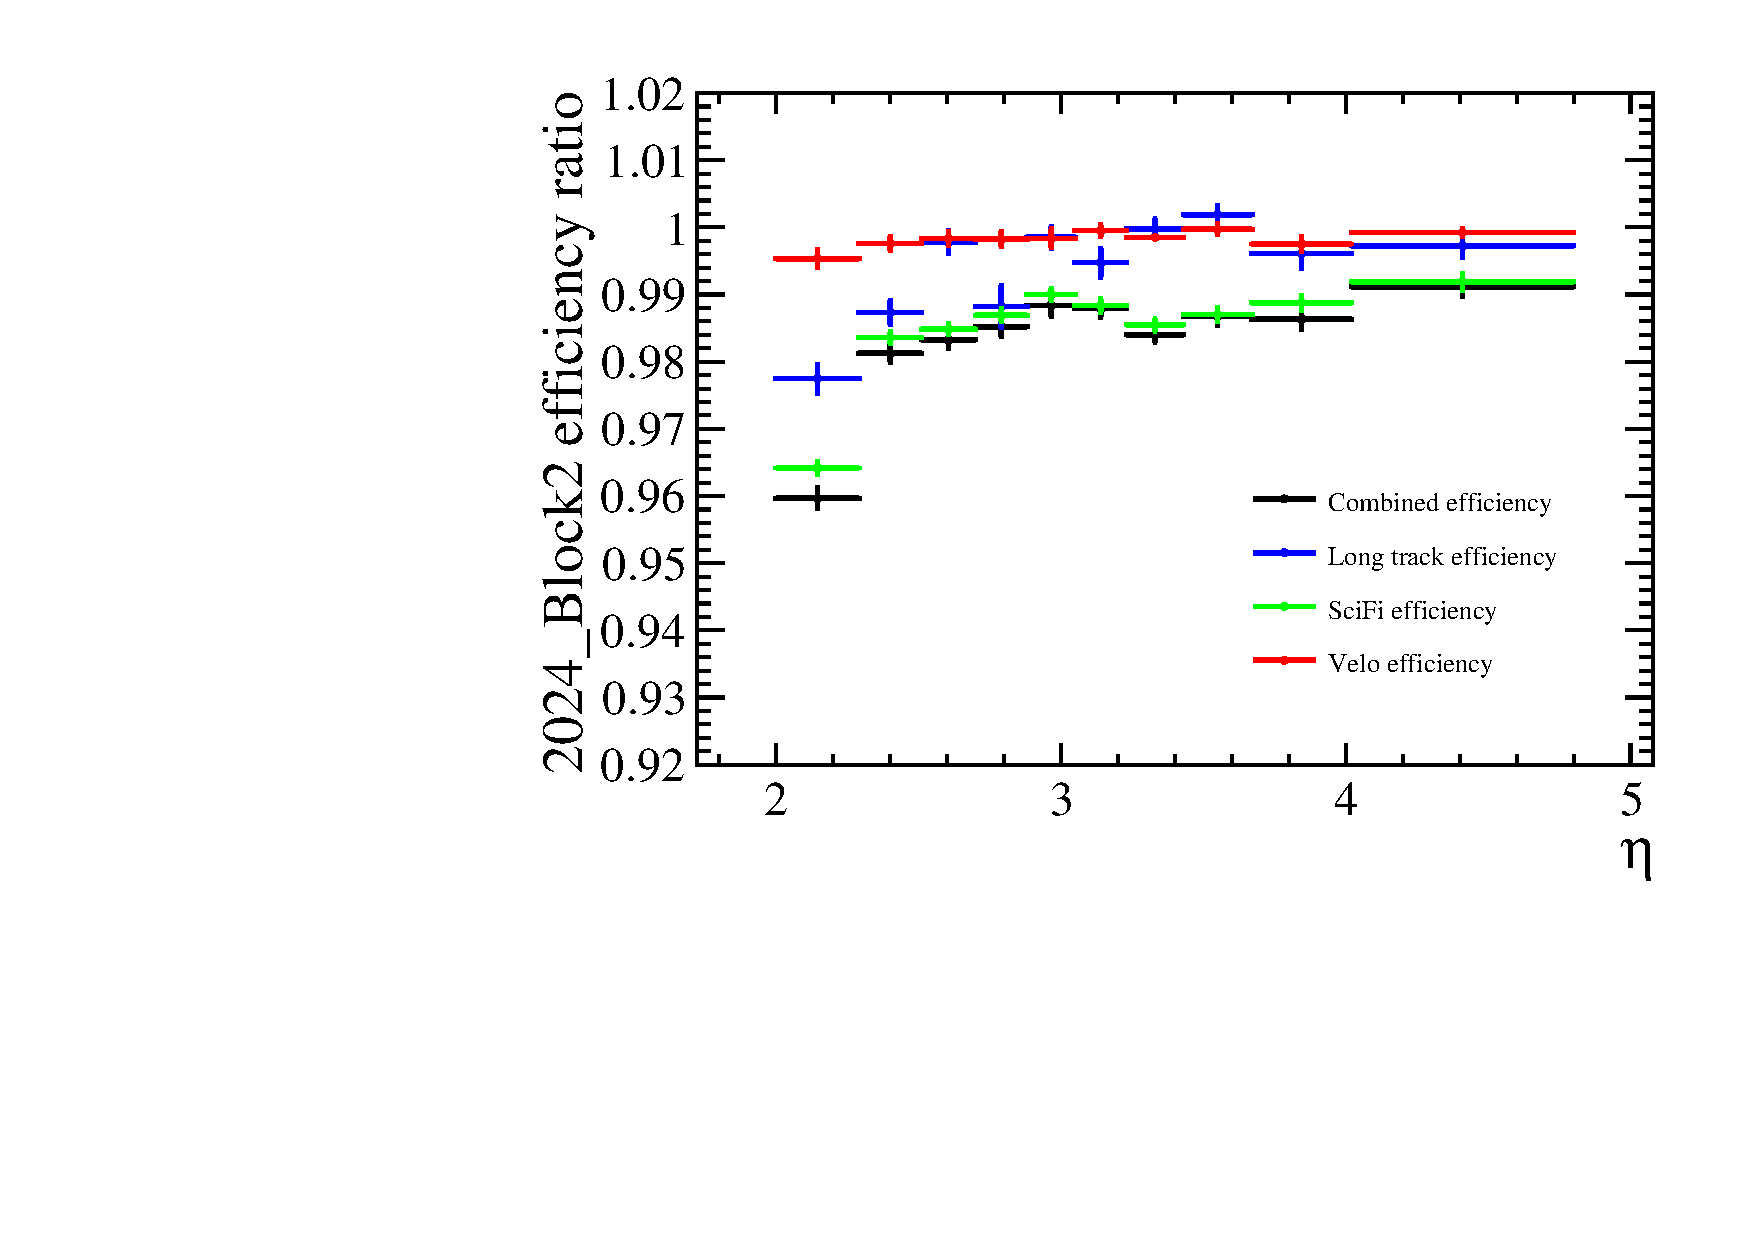
\includegraphics[width=1.0\textwidth]{Plots/trackeff_ratio_ETA_2024_Block2_default_samples.pdf}
    \end{subfigure}%
    \begin{subfigure}{0.5\textwidth}
      \centering
      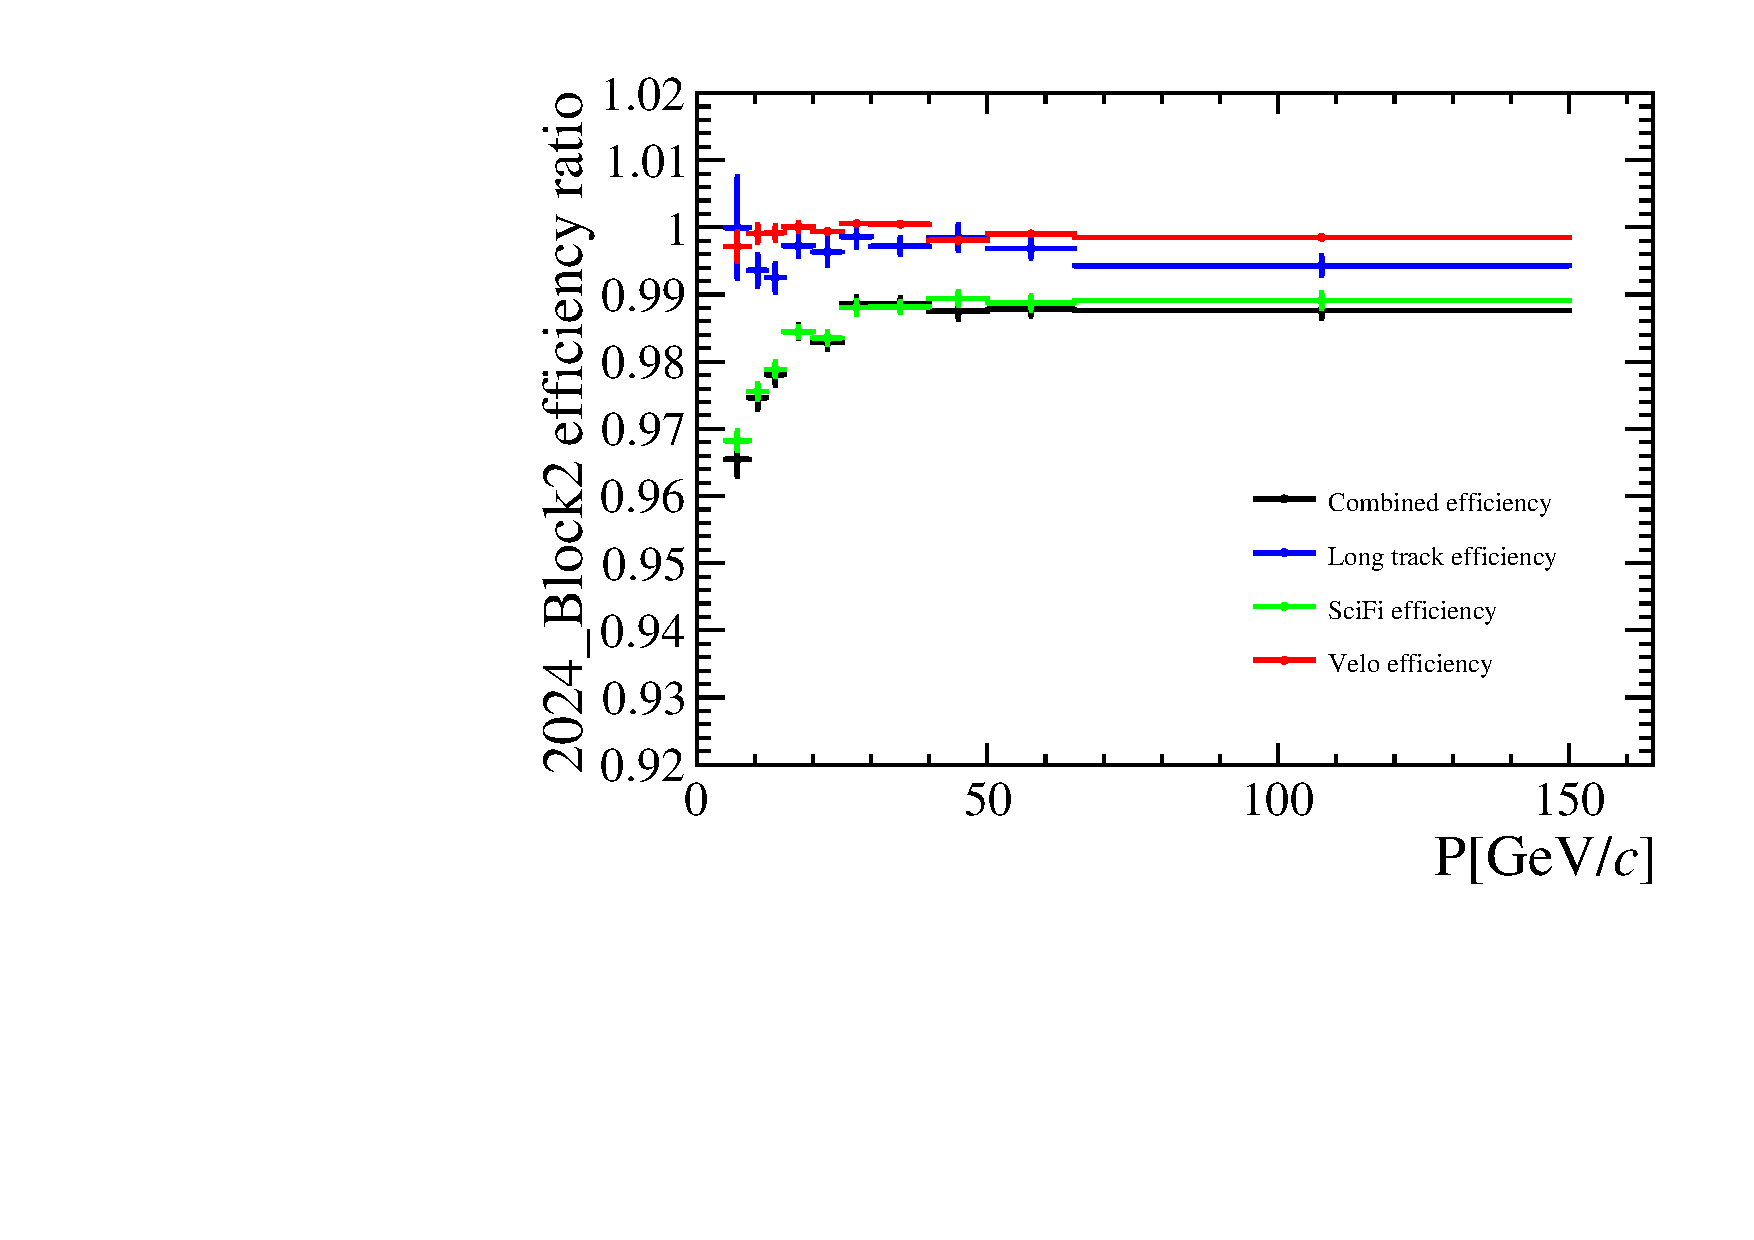
\includegraphics[width=1.0\textwidth]{Plots/trackeff_ratio_P_2024_Block2_default_samples.pdf}
    \end{subfigure}
  \end{figure}
  {Data/MC ratio for Combined/MuonUT track efficiencies block 2}
\end{frame}

\begin{frame}{Tracking efficiency data/MC ratio}
  \vspace{0.0cm}
  {\large Data/MC ratio}
  \begin{figure}[htb]
    \centering
    \begin{subfigure}{0.5\textwidth}
      \centering
      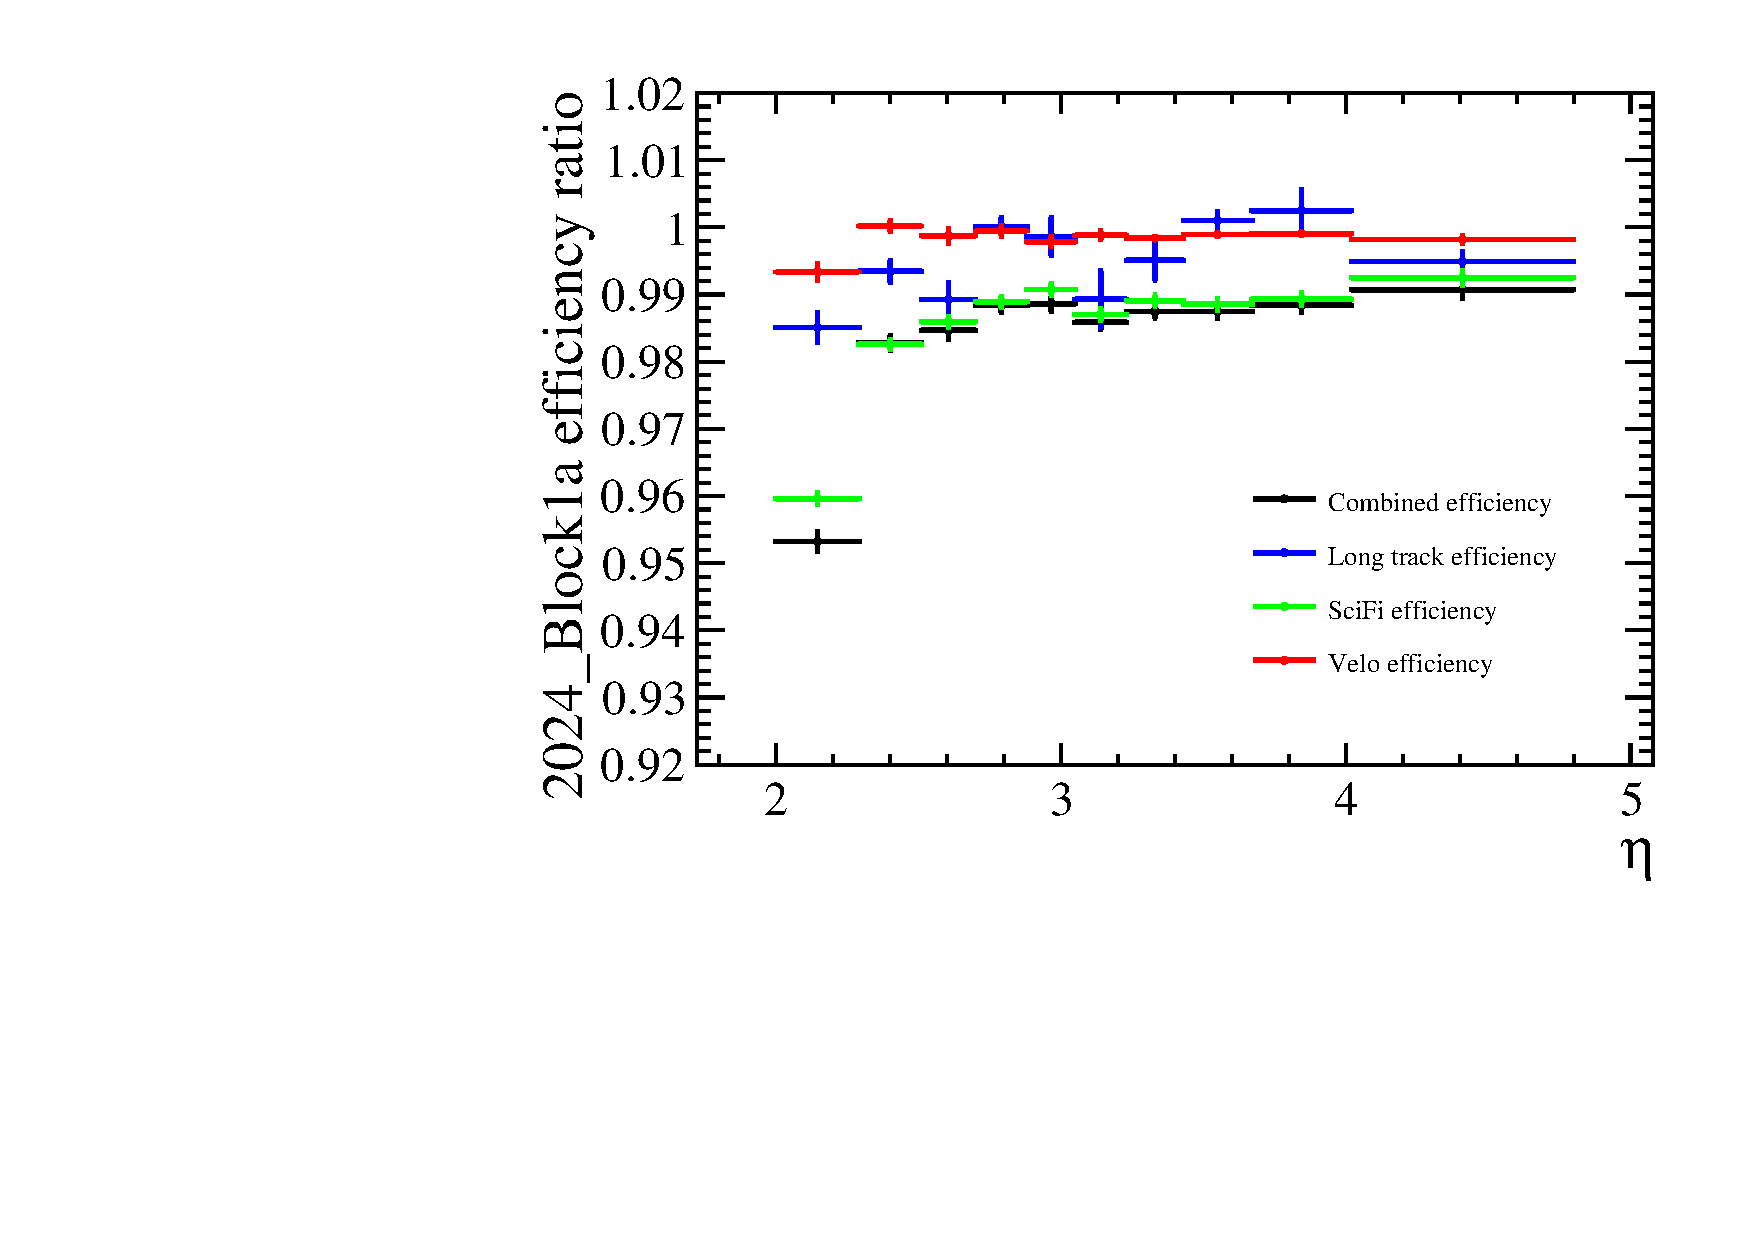
\includegraphics[width=1.0\textwidth]{Plots/trackeff_ratio_ETA_2024_Block1a_default_samples.pdf}
    \end{subfigure}%
    \begin{subfigure}{0.5\textwidth}
      \centering
      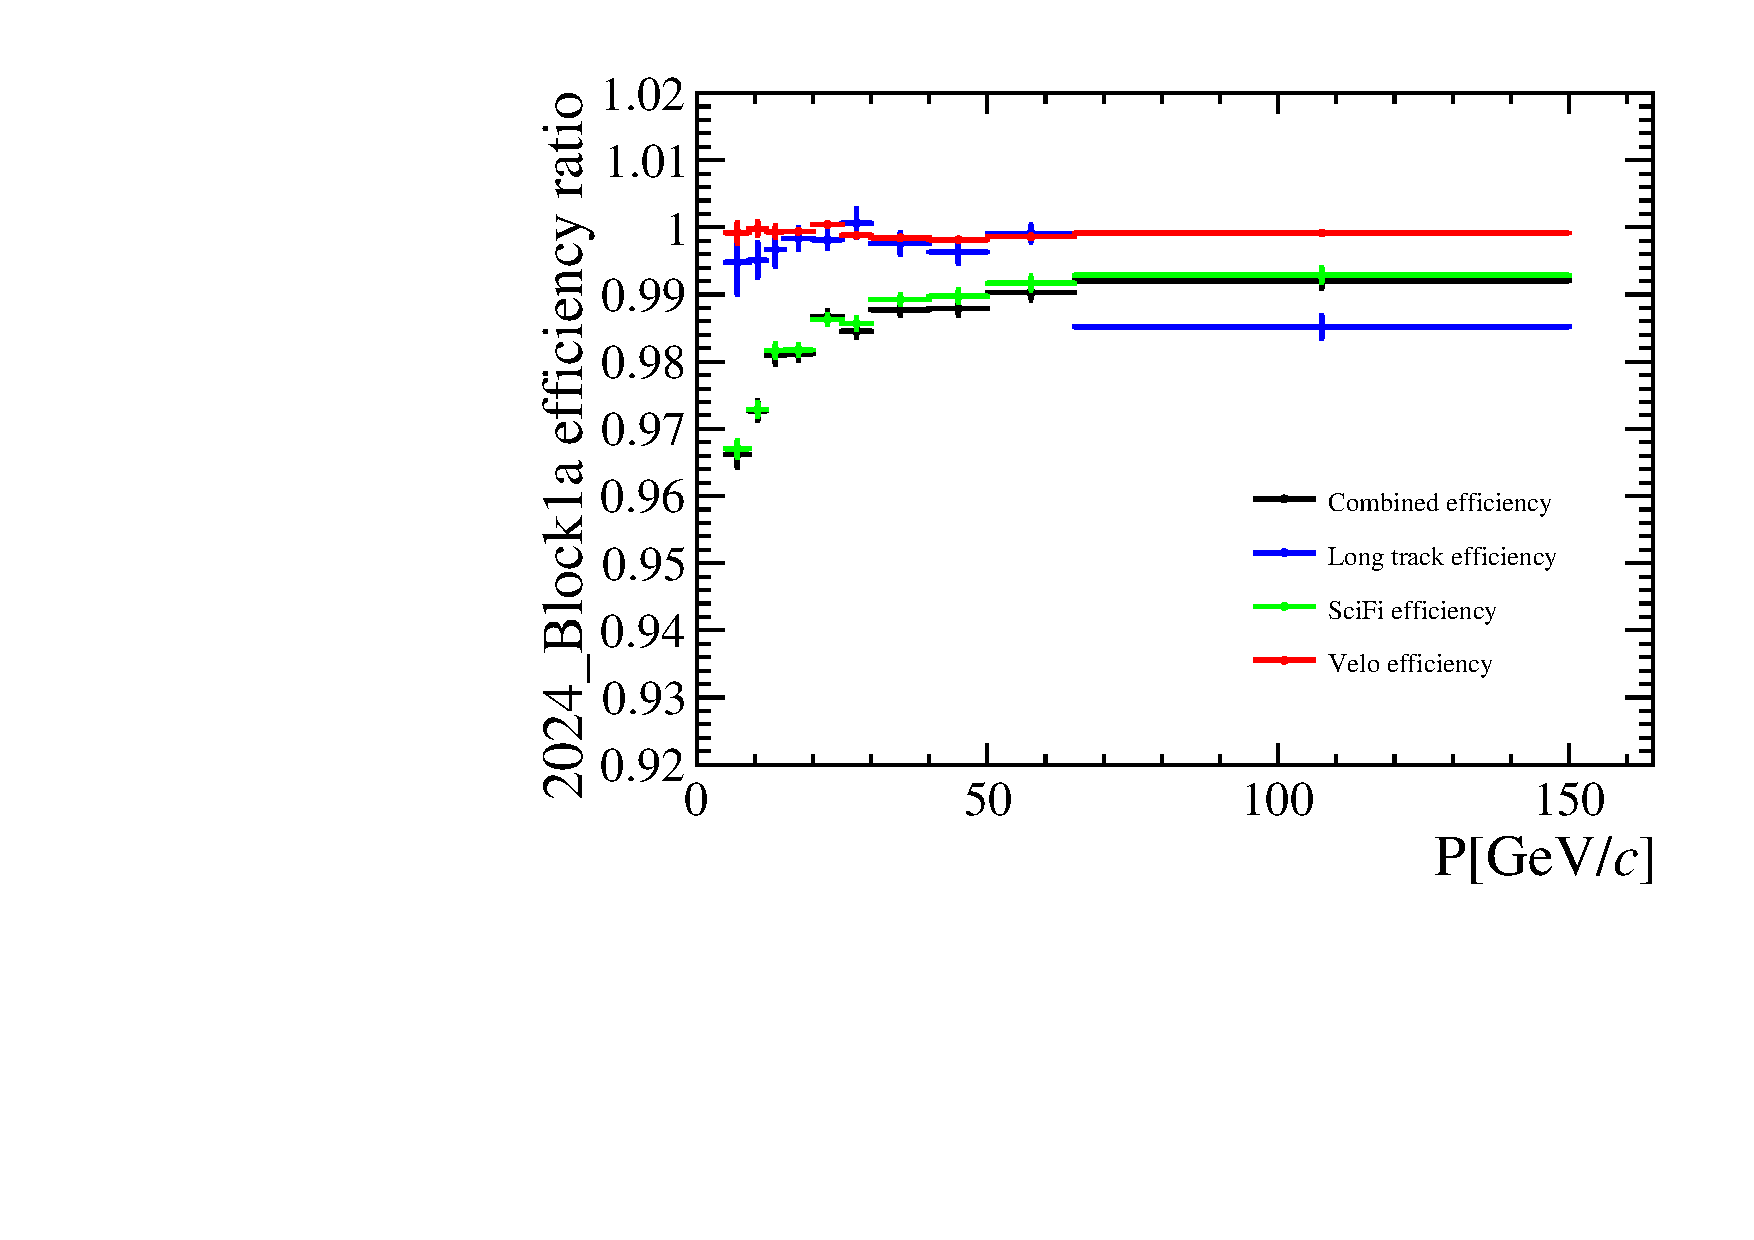
\includegraphics[width=1.0\textwidth]{Plots/trackeff_ratio_P_2024_Block1a_default_samples.pdf}
    \end{subfigure}
  \end{figure}
  {Data/MC ratio for Combined/MuonUT track efficiencies block 1a}
\end{frame}

\begin{frame}{Tracking efficiency data/MC ratio}
  \vspace{0.0cm}
  {\large Data/MC ratio}
  \begin{figure}[htb]
    \centering
    \begin{subfigure}{0.5\textwidth}
      \centering
      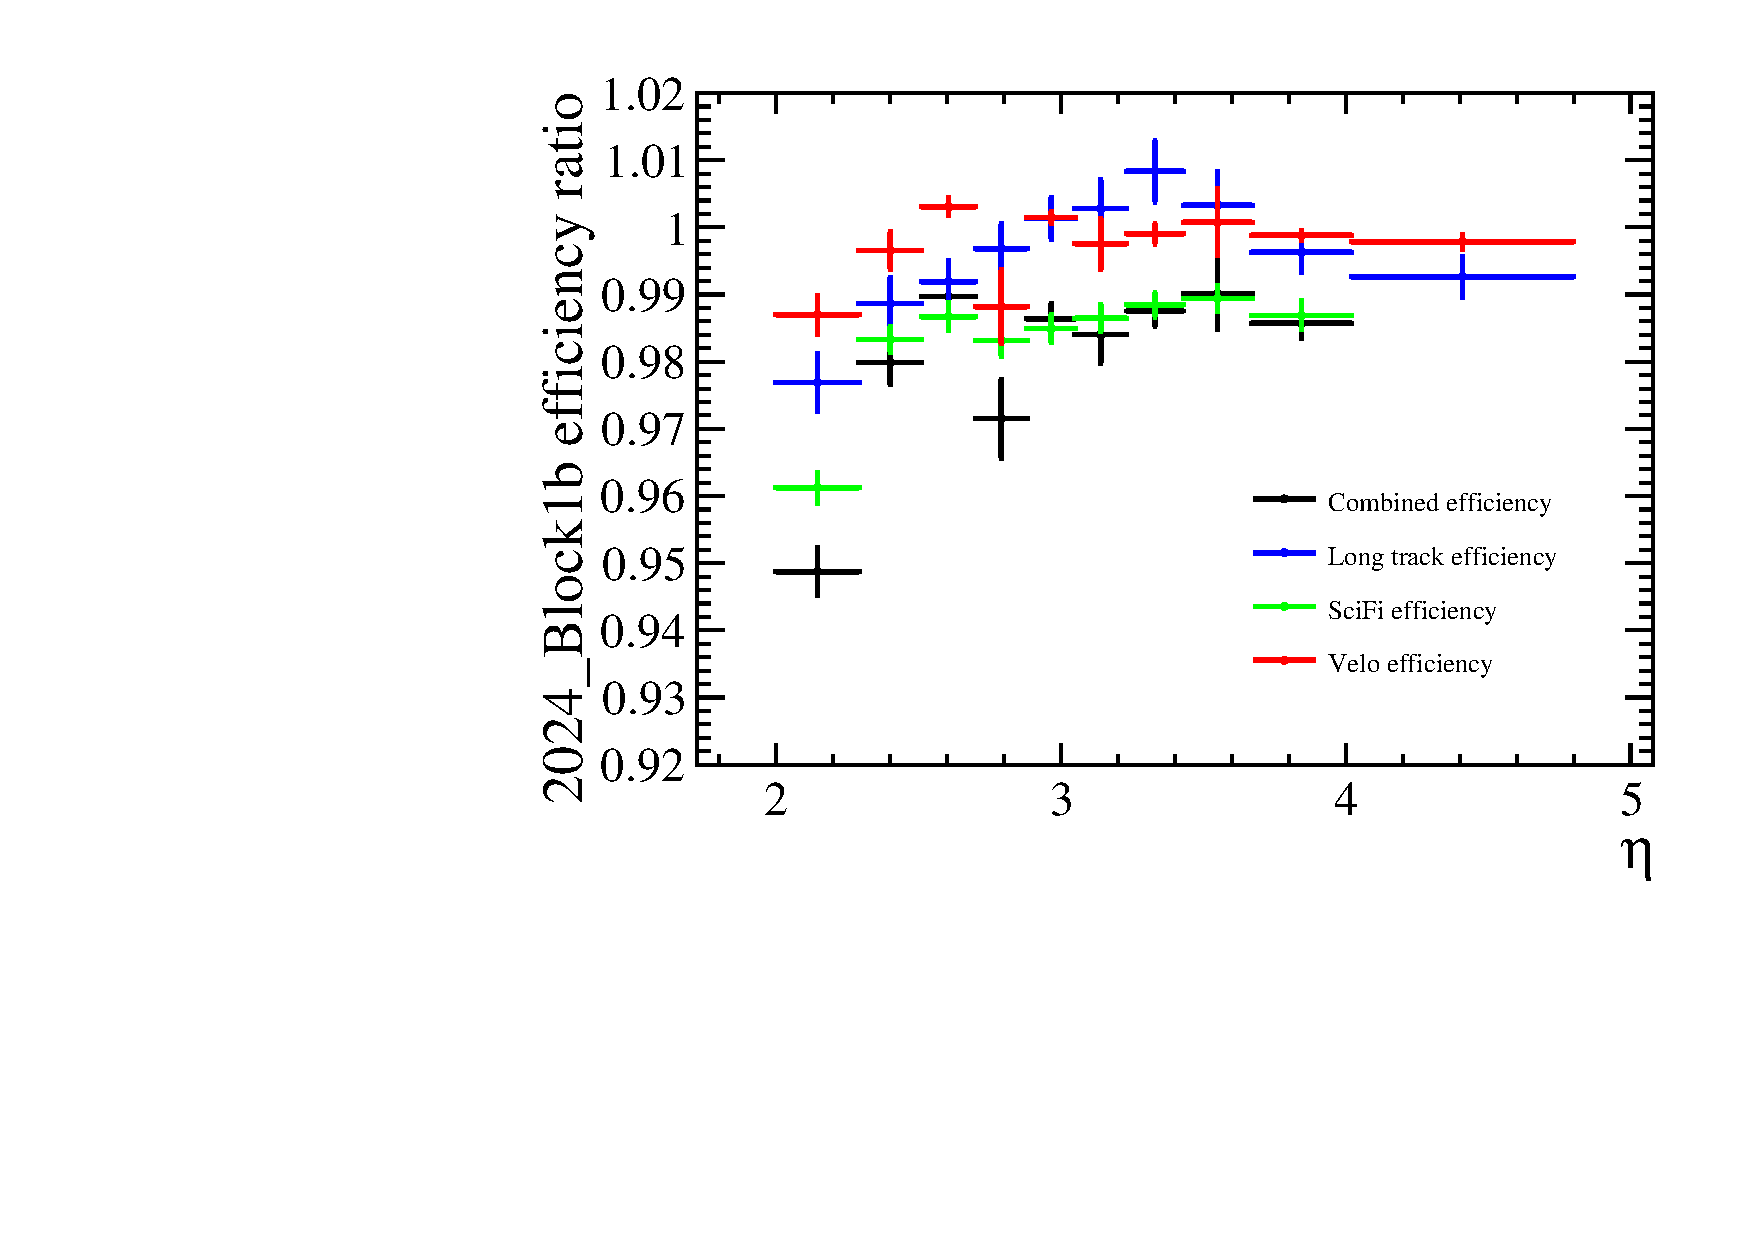
\includegraphics[width=1.0\textwidth]{Plots/trackeff_ratio_ETA_2024_Block1b_default_samples.pdf}
    \end{subfigure}%
    \begin{subfigure}{0.5\textwidth}
      \centering
      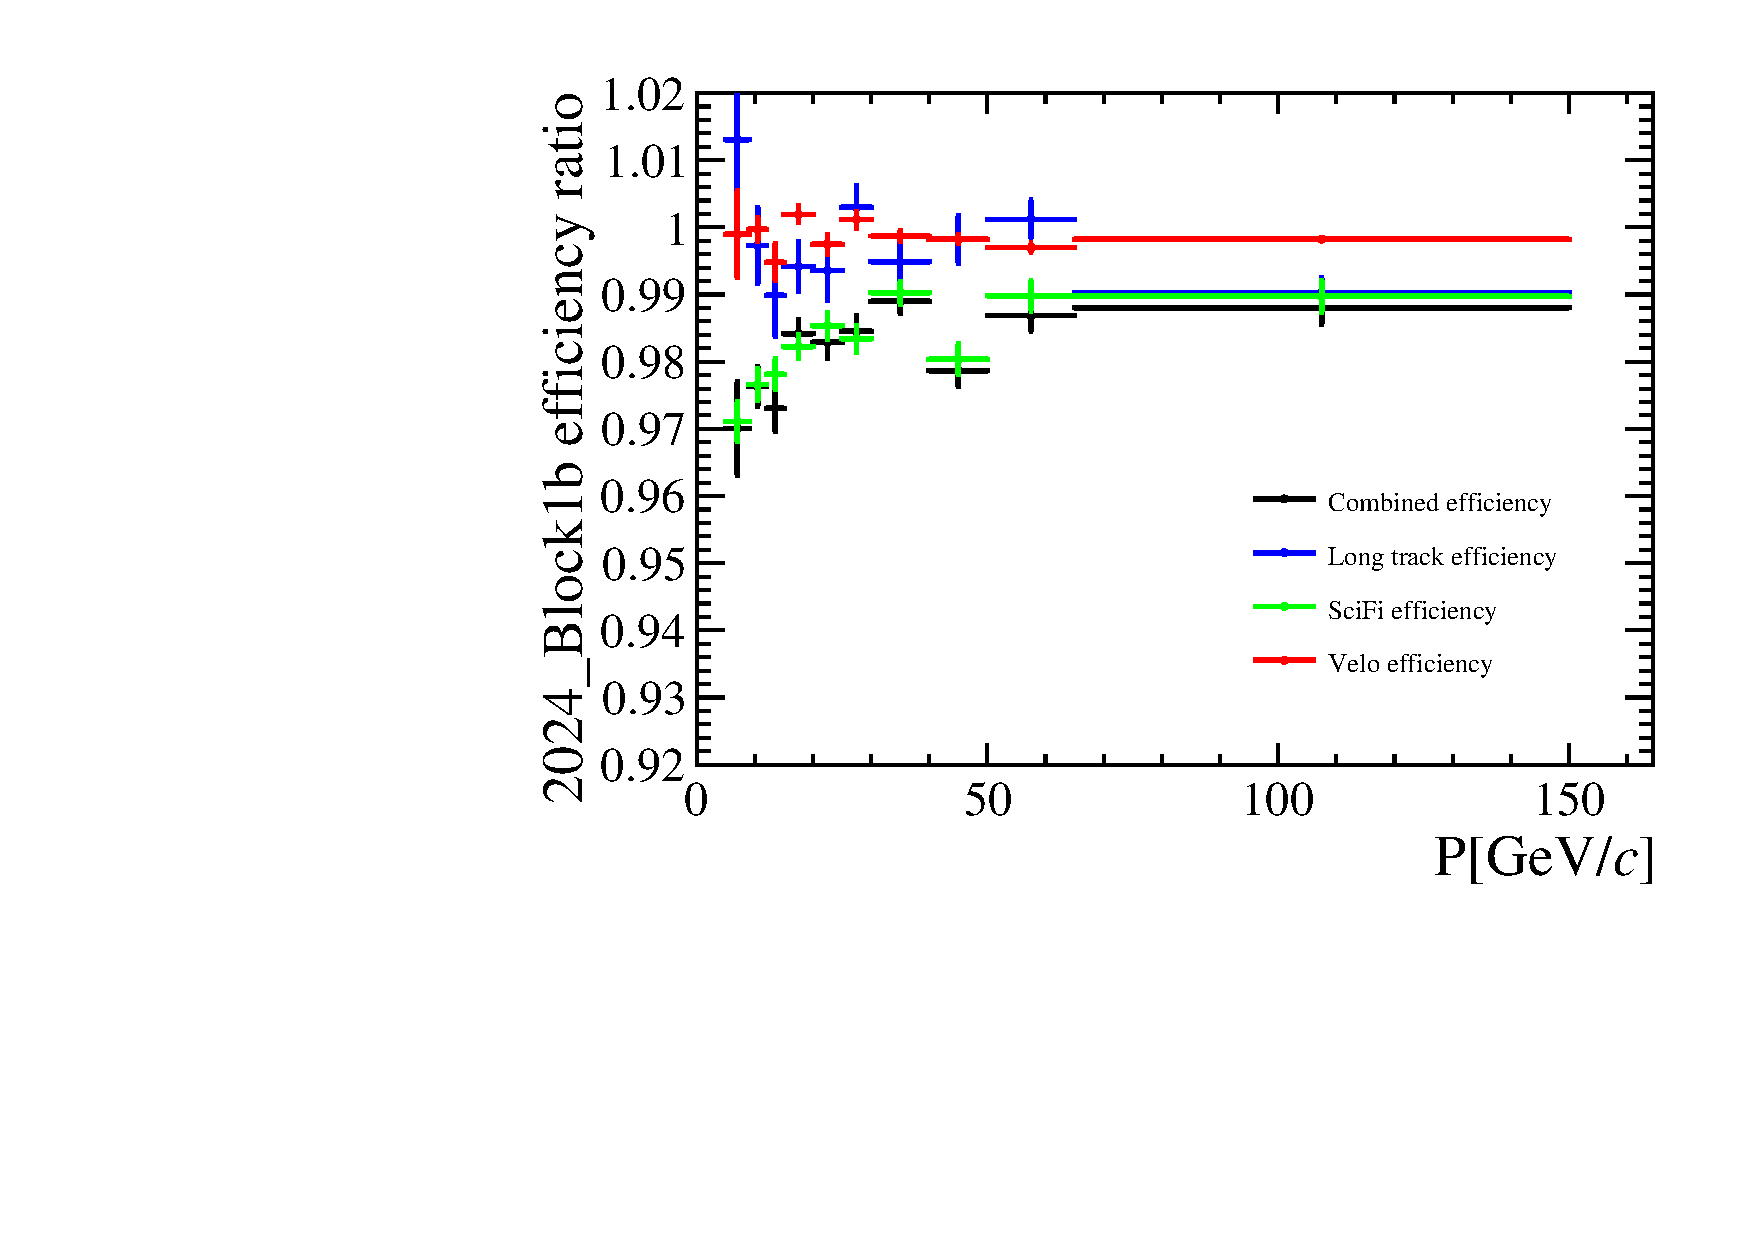
\includegraphics[width=1.0\textwidth]{Plots/trackeff_ratio_P_2024_Block1b_default_samples.pdf}
    \end{subfigure}
  \end{figure}
  {Data/MC ratio for Combined/MuonUT track efficiencies block 1b}
\end{frame}

\begin{frame}{Tracking efficiency data/MC ratio}
  \vspace{0.0cm}
  {\large Data/MC ratio}
  \begin{figure}[htb]
    \centering
    \begin{subfigure}{0.5\textwidth}
      \centering
      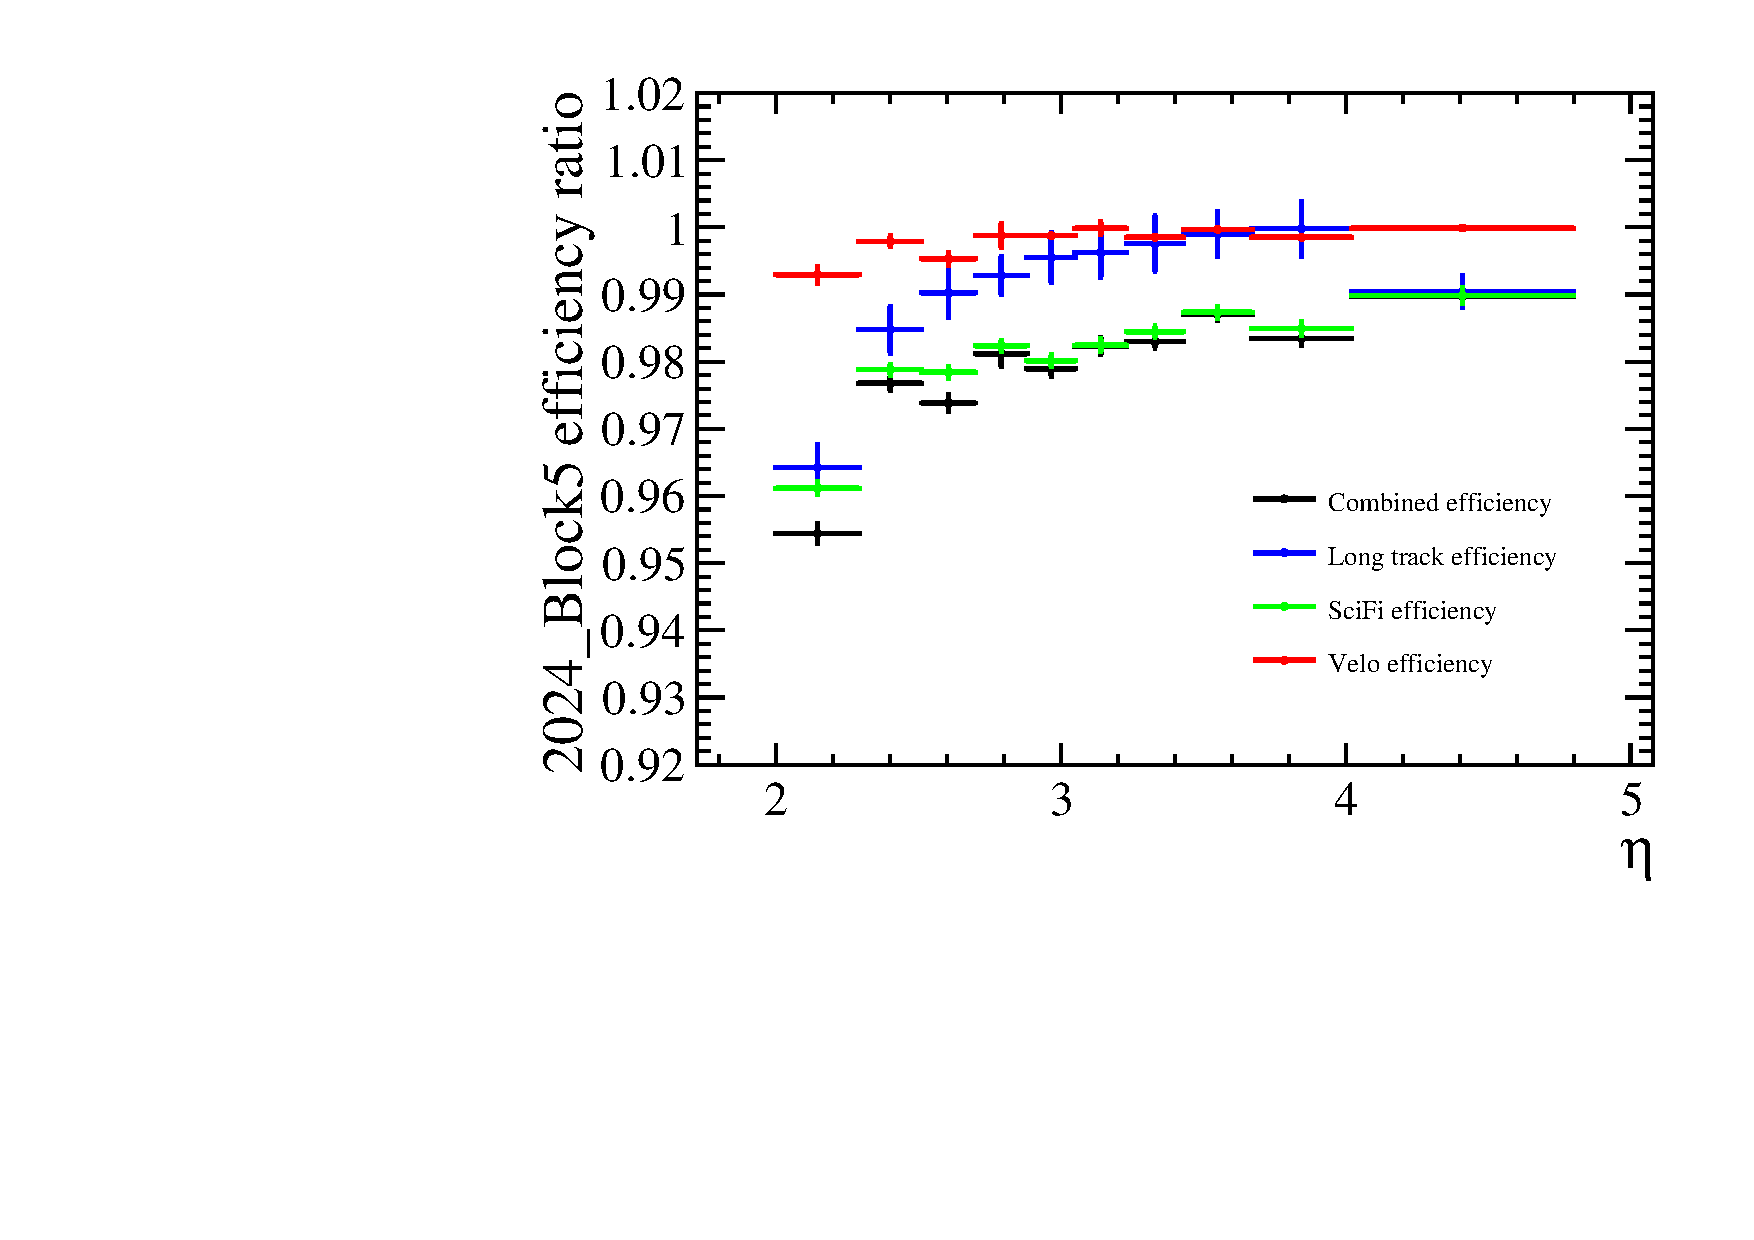
\includegraphics[width=1.0\textwidth]{Plots/trackeff_ratio_ETA_2024_Block5_default_samples.pdf}
    \end{subfigure}%
    \begin{subfigure}{0.5\textwidth}
      \centering
      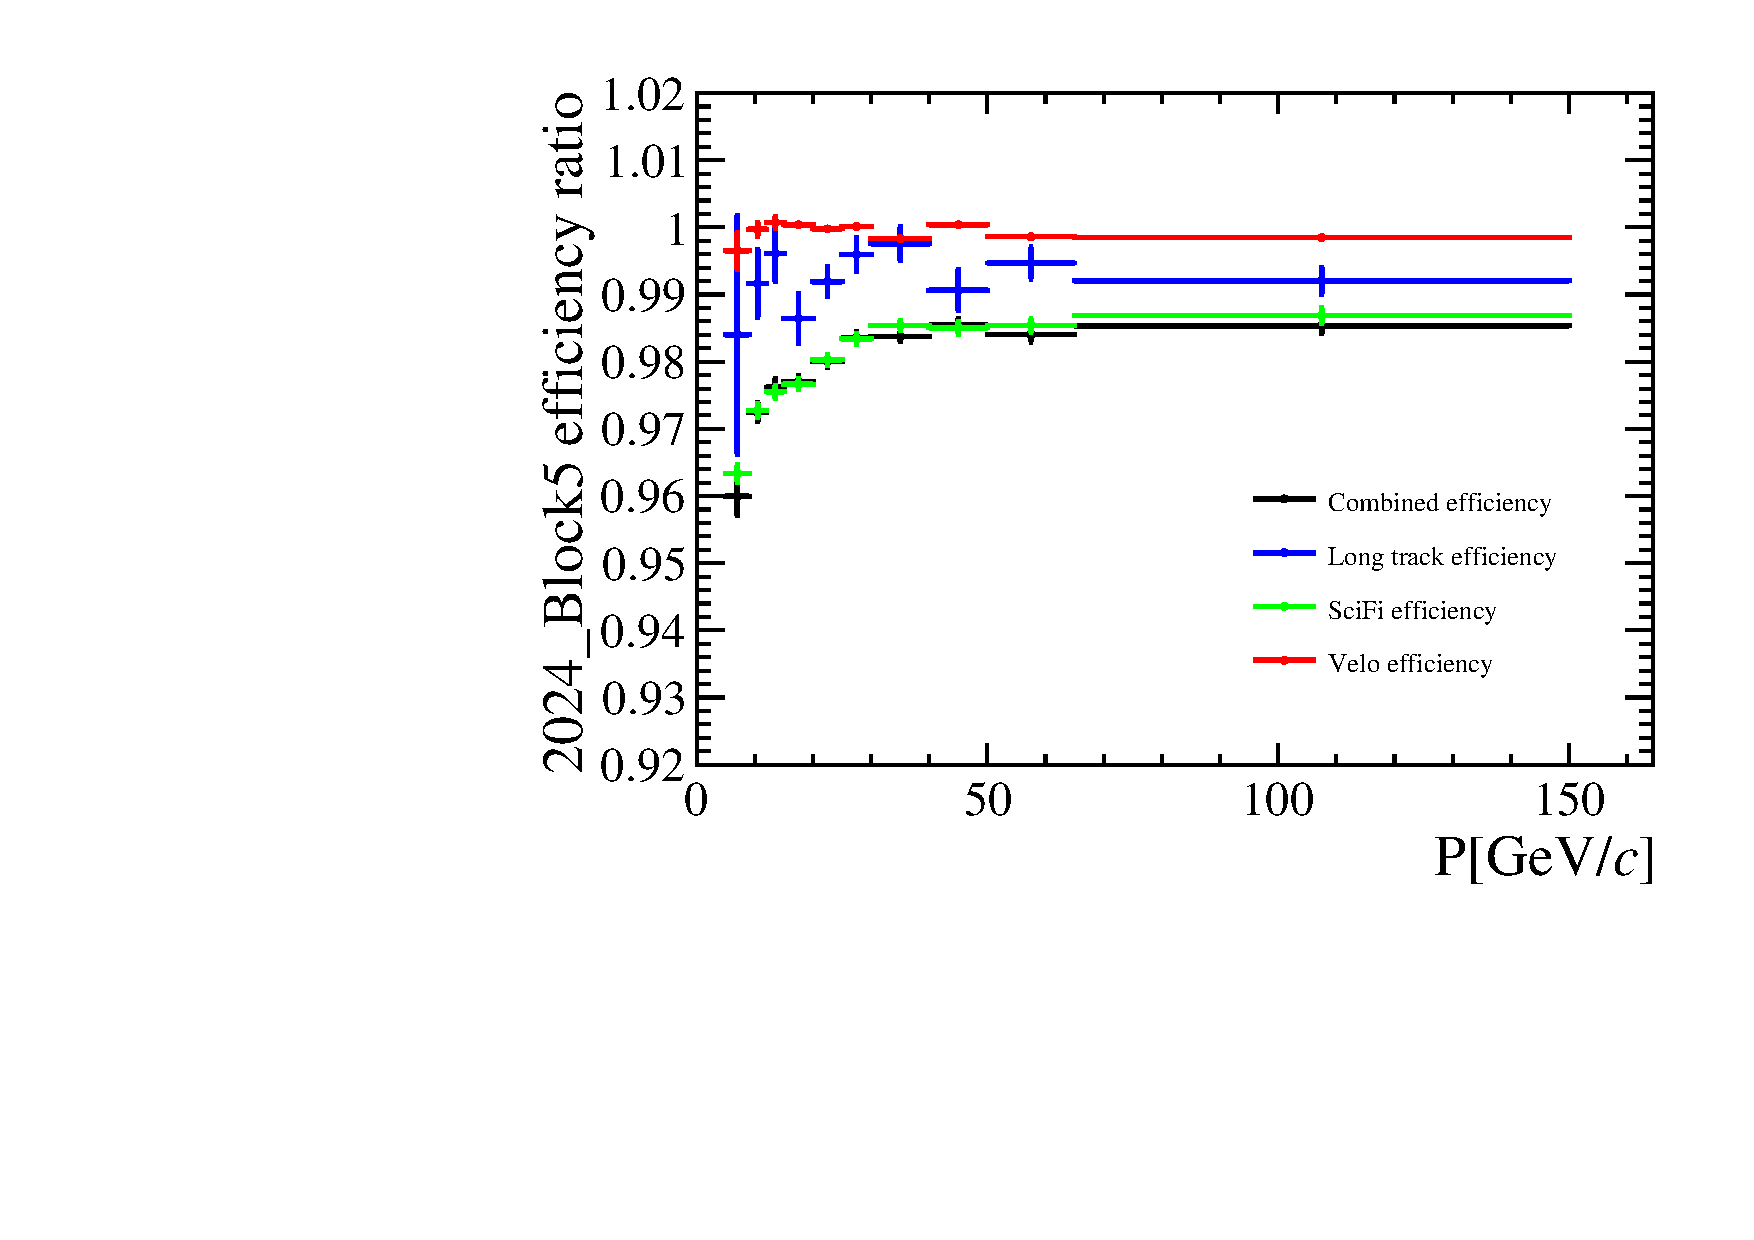
\includegraphics[width=1.0\textwidth]{Plots/trackeff_ratio_P_2024_Block5_default_samples.pdf}
    \end{subfigure}
  \end{figure}
  {Data/MC ratio for Combined/MuonUT track efficiencies block 5}
\end{frame}

\begin{frame}{Tracking efficiency data/MC ratio}
  \vspace{0.0cm}
  {\large Data/MC ratio}
  \begin{figure}[htb]
    \centering
    \begin{subfigure}{0.5\textwidth}
      \centering
      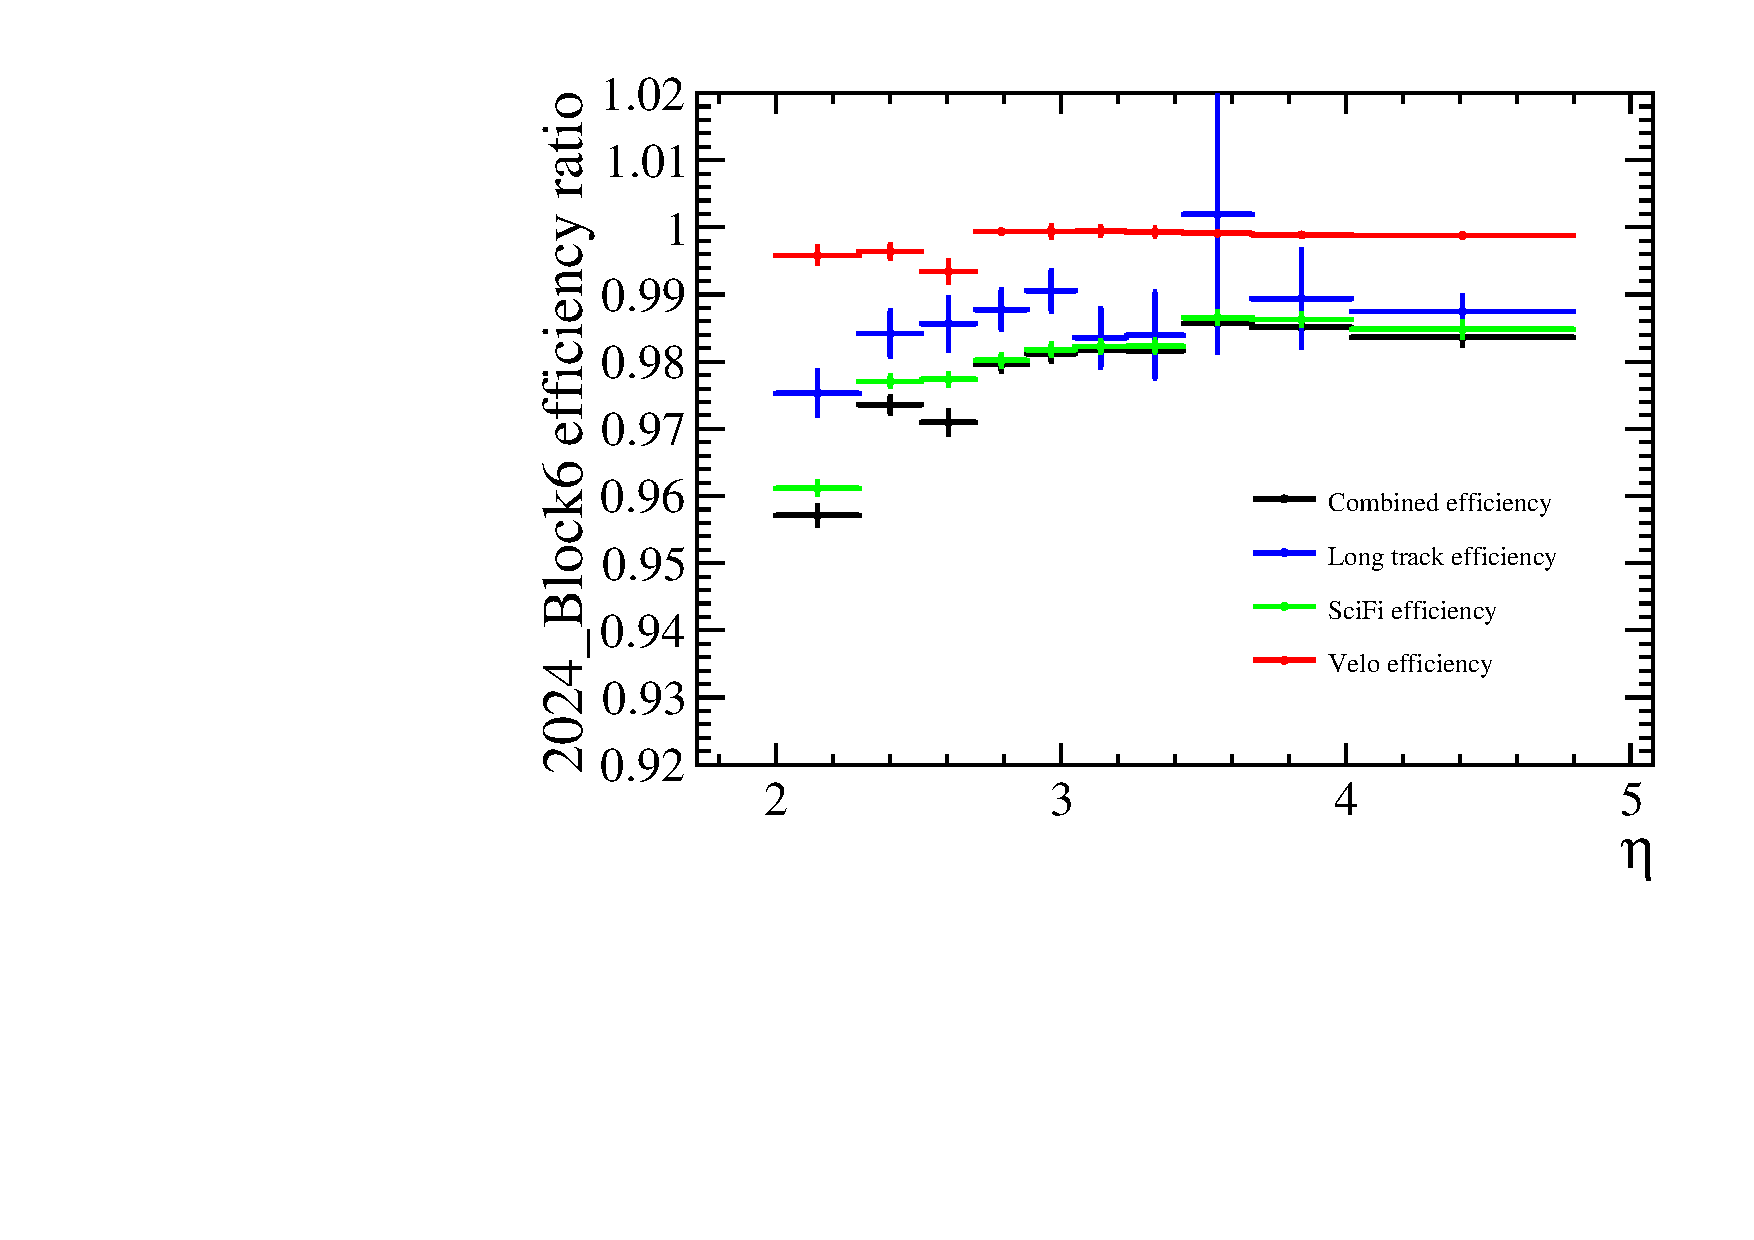
\includegraphics[width=1.0\textwidth]{Plots/trackeff_ratio_ETA_2024_Block6_default_samples.pdf}
    \end{subfigure}%
    \begin{subfigure}{0.5\textwidth}
      \centering
      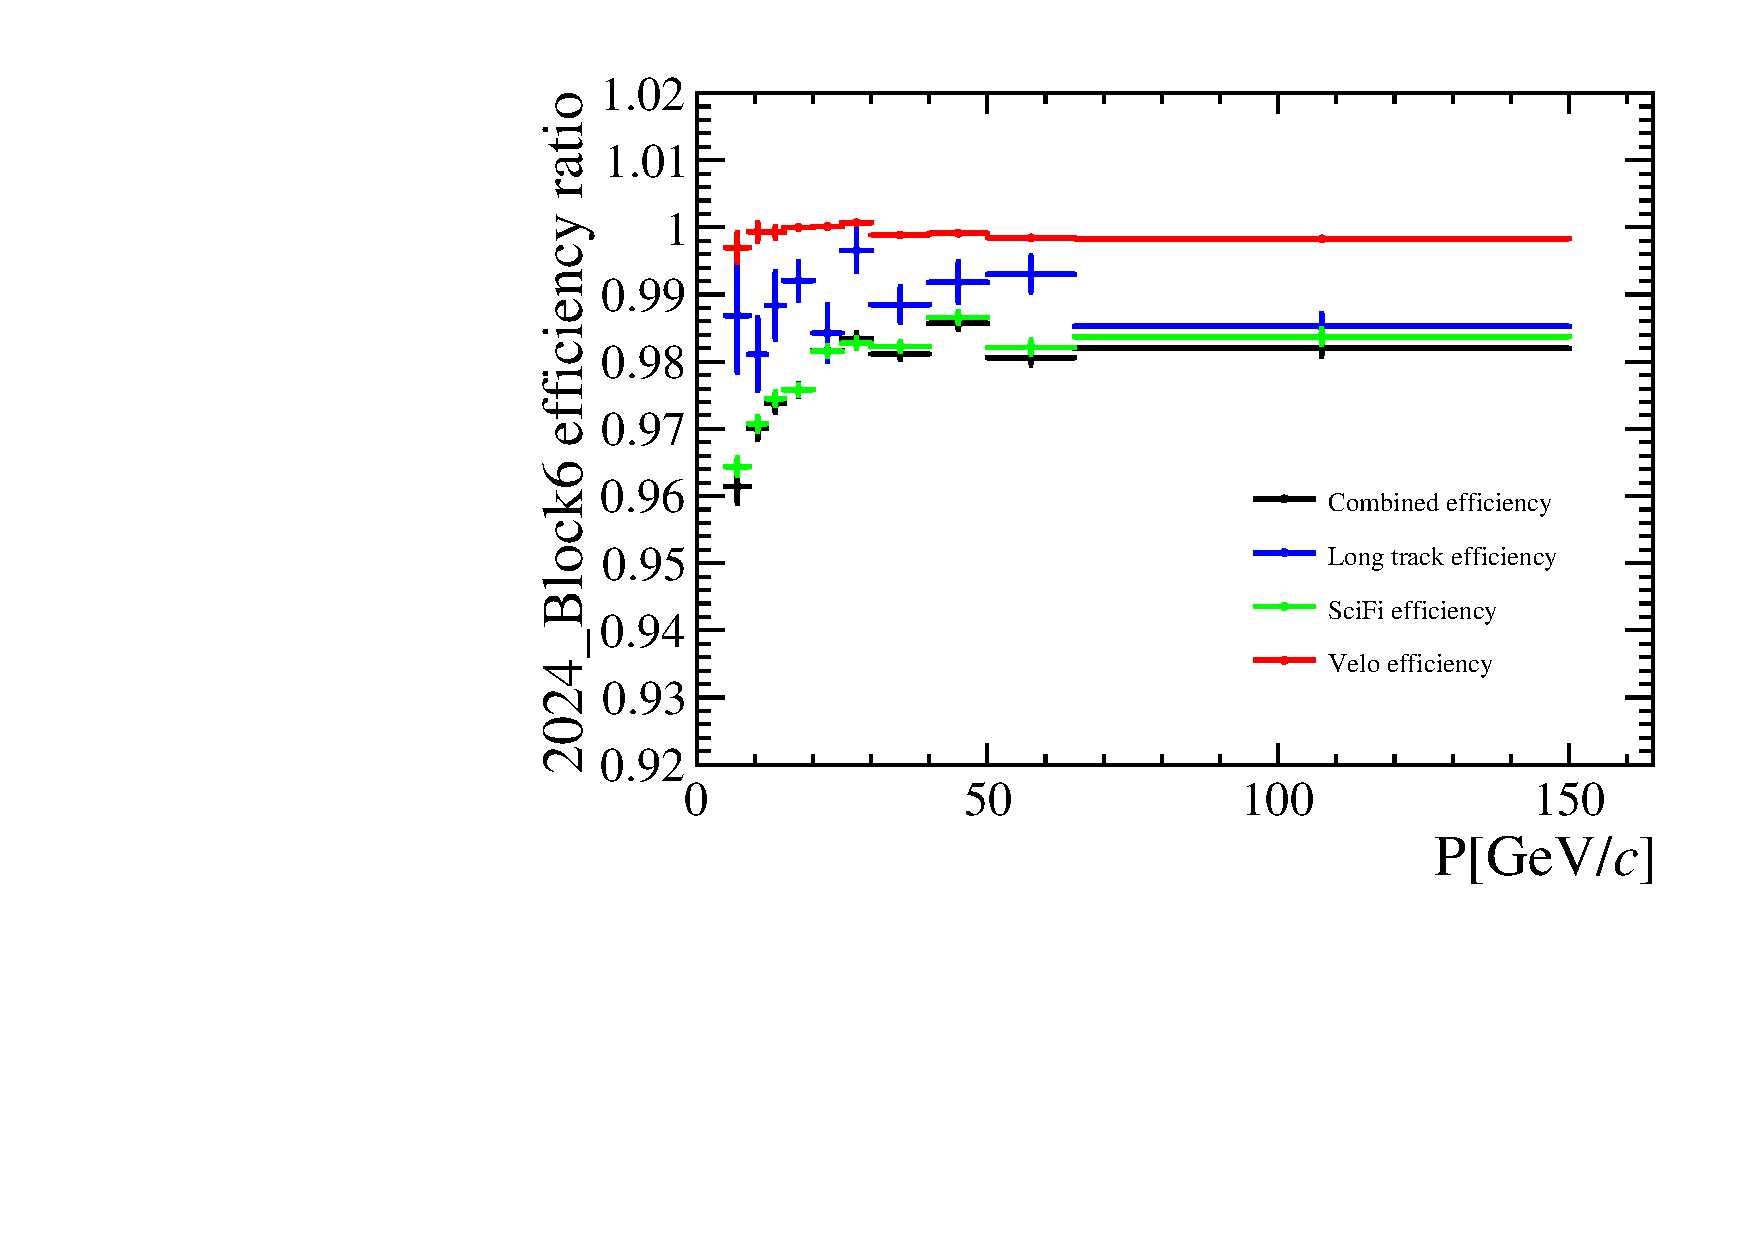
\includegraphics[width=1.0\textwidth]{Plots/trackeff_ratio_P_2024_Block6_default_samples.pdf}
    \end{subfigure}
  \end{figure}
  {Data/MC ratio for Combined/MuonUT track efficiencies block 6}
\end{frame}

\begin{frame}{Tracking efficiency data/MC ratio}
  \vspace{0.0cm}
  {\large Data/MC ratio}
  \begin{figure}[htb]
    \centering
    \begin{subfigure}{0.5\textwidth}
      \centering
      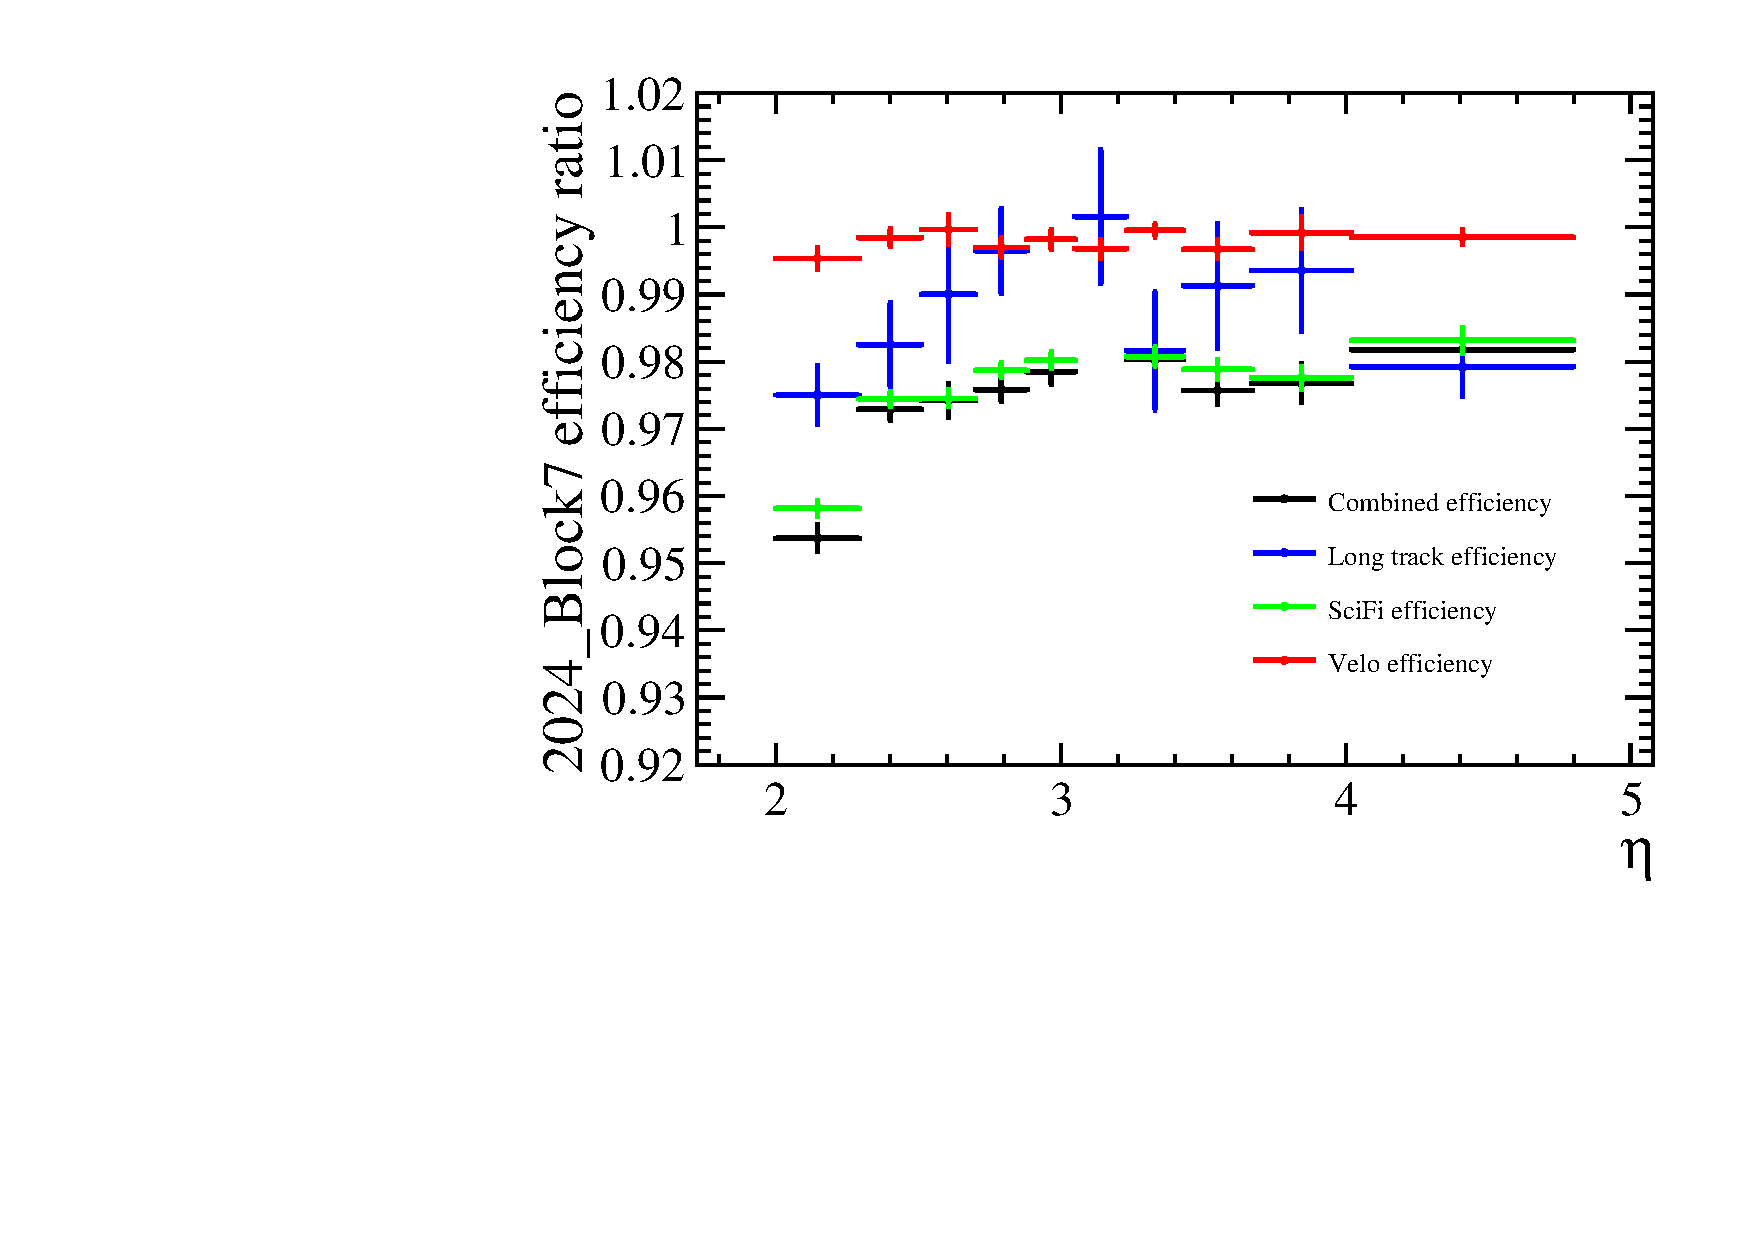
\includegraphics[width=1.0\textwidth]{Plots/trackeff_ratio_ETA_2024_Block7_default_samples.pdf}
    \end{subfigure}%
    \begin{subfigure}{0.5\textwidth}
      \centering
      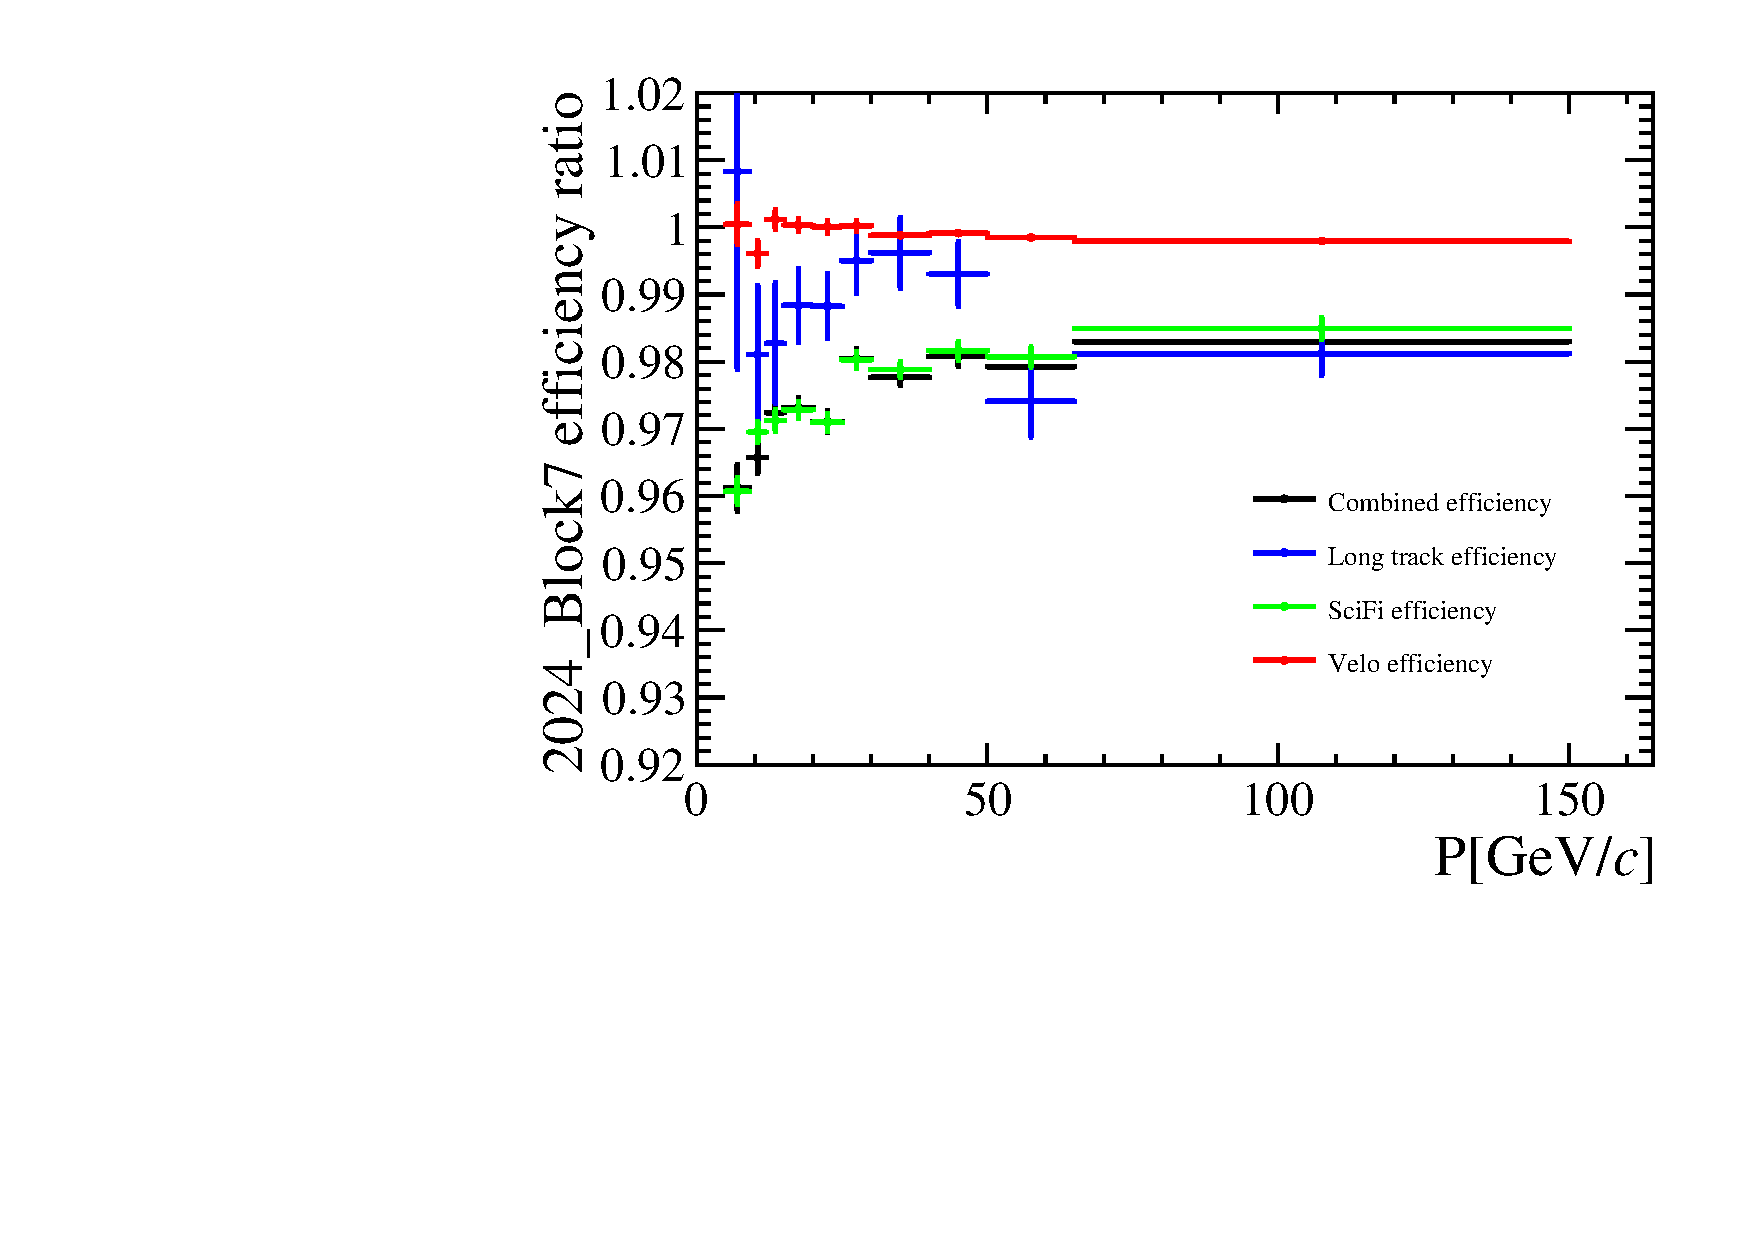
\includegraphics[width=1.0\textwidth]{Plots/trackeff_ratio_P_2024_Block7_default_samples.pdf}
    \end{subfigure}
  \end{figure}
  {Data/MC ratio for Combined/MuonUT track efficiencies block 7}
\end{frame}

\begin{frame}{Tracking efficiency data/MC ratio}
  \vspace{0.0cm}
  {\large Data/MC ratio}
  \begin{figure}[htb]
    \centering
    \begin{subfigure}{0.5\textwidth}
      \centering
      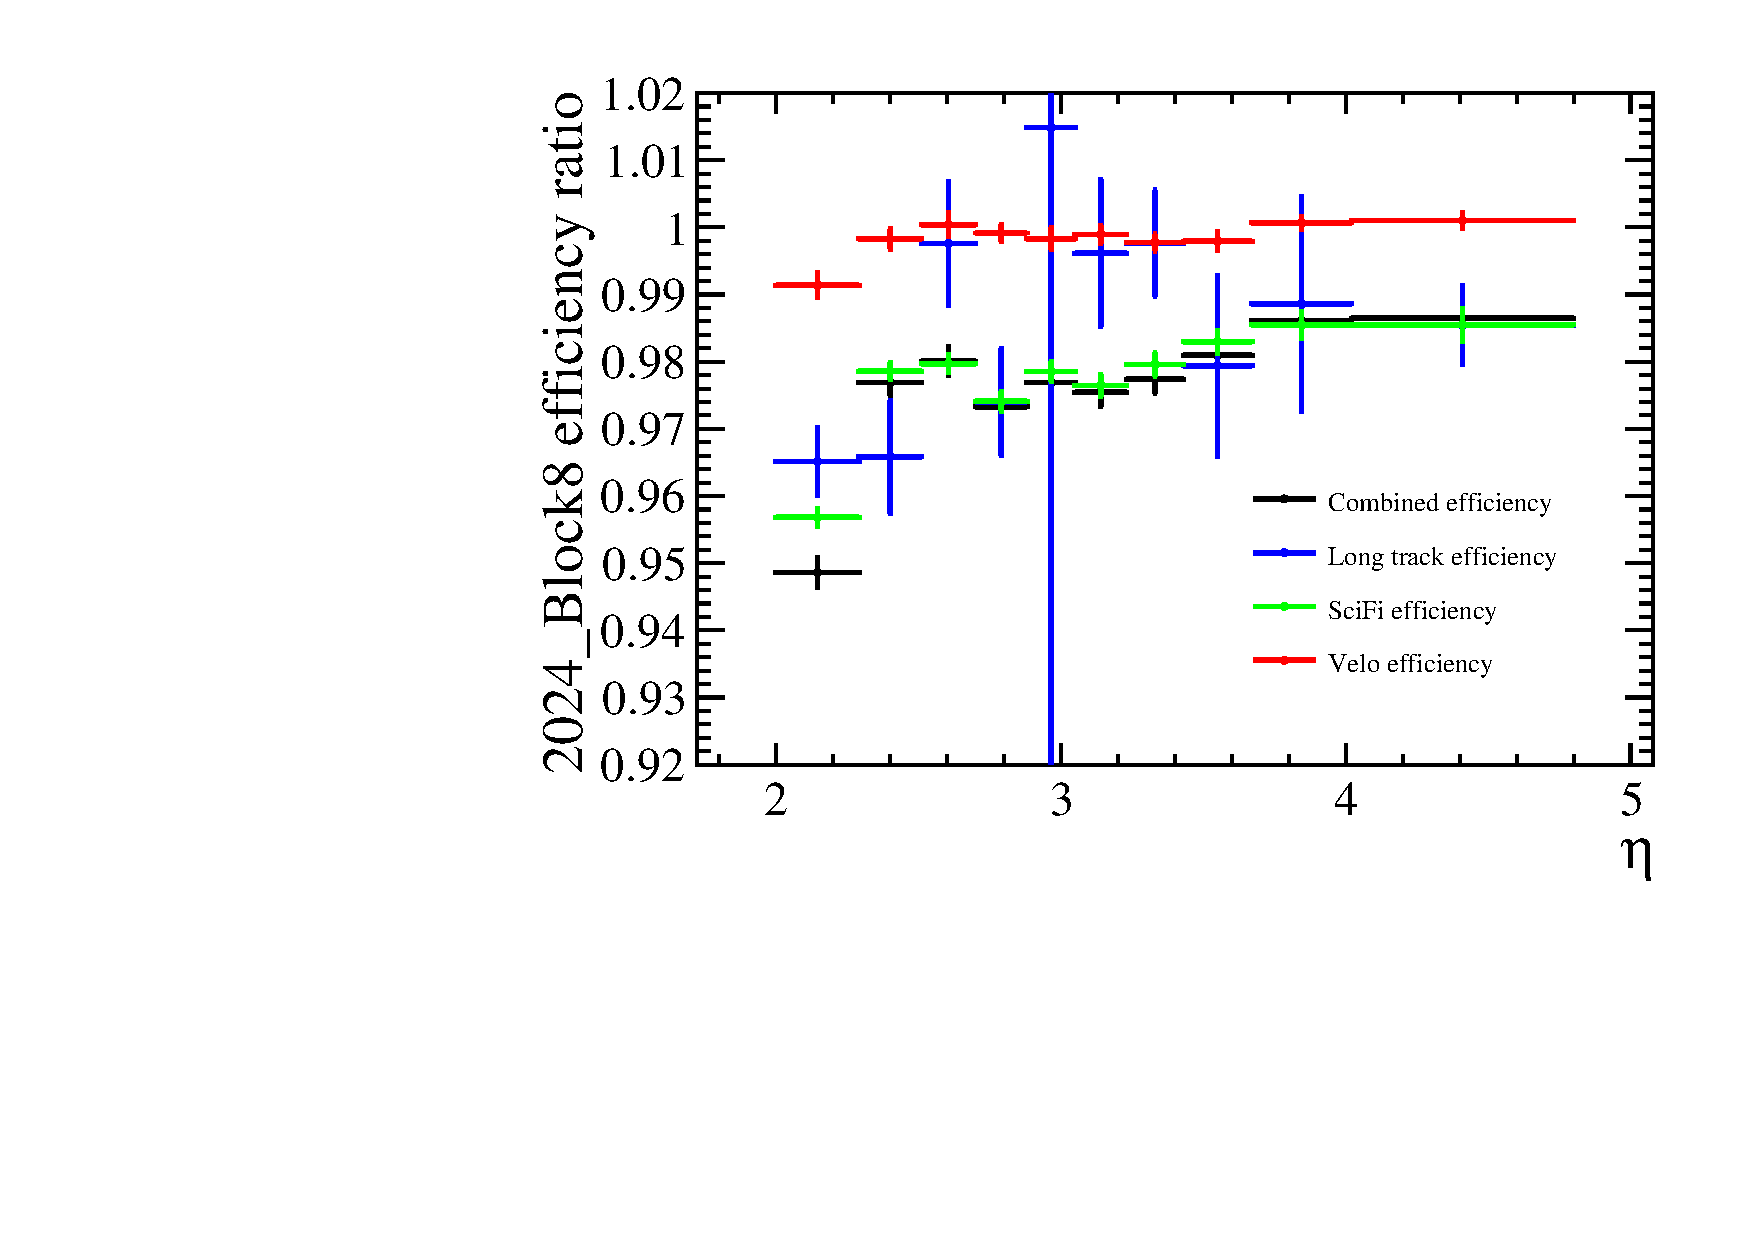
\includegraphics[width=1.0\textwidth]{Plots/trackeff_ratio_ETA_2024_Block8_default_samples.pdf}
    \end{subfigure}%
    \begin{subfigure}{0.5\textwidth}
      \centering
      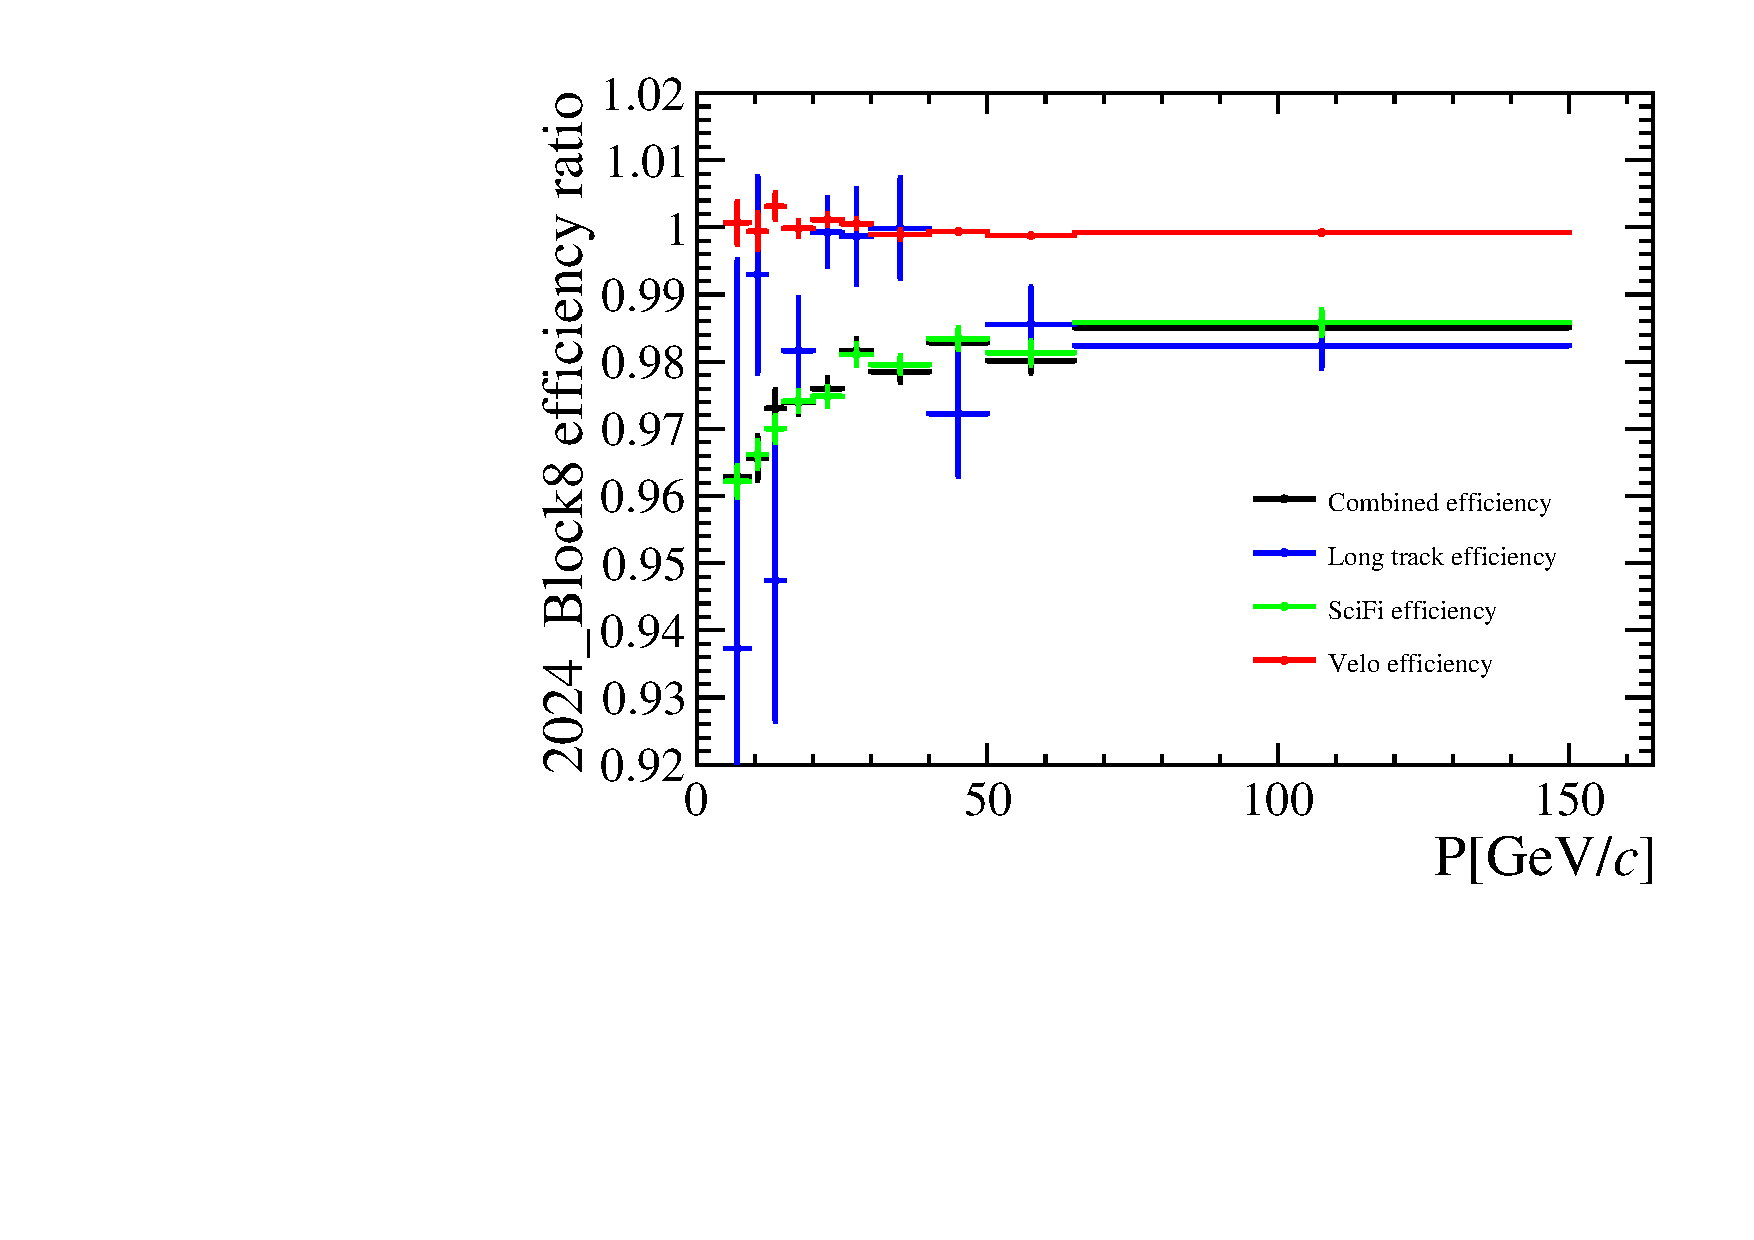
\includegraphics[width=1.0\textwidth]{Plots/trackeff_ratio_P_2024_Block8_default_samples.pdf}
    \end{subfigure}
  \end{figure}
  {Data/MC ratio for Combined/MuonUT track efficiencies block 8}
\end{frame}

\begin{frame}{Tracking efficiency data/MC ratio}
  \vspace{0.0cm}
  {\large Data/MC ratio}
  \begin{figure}[htb]
    \centering
    \begin{subfigure}{0.5\textwidth}
      \centering
      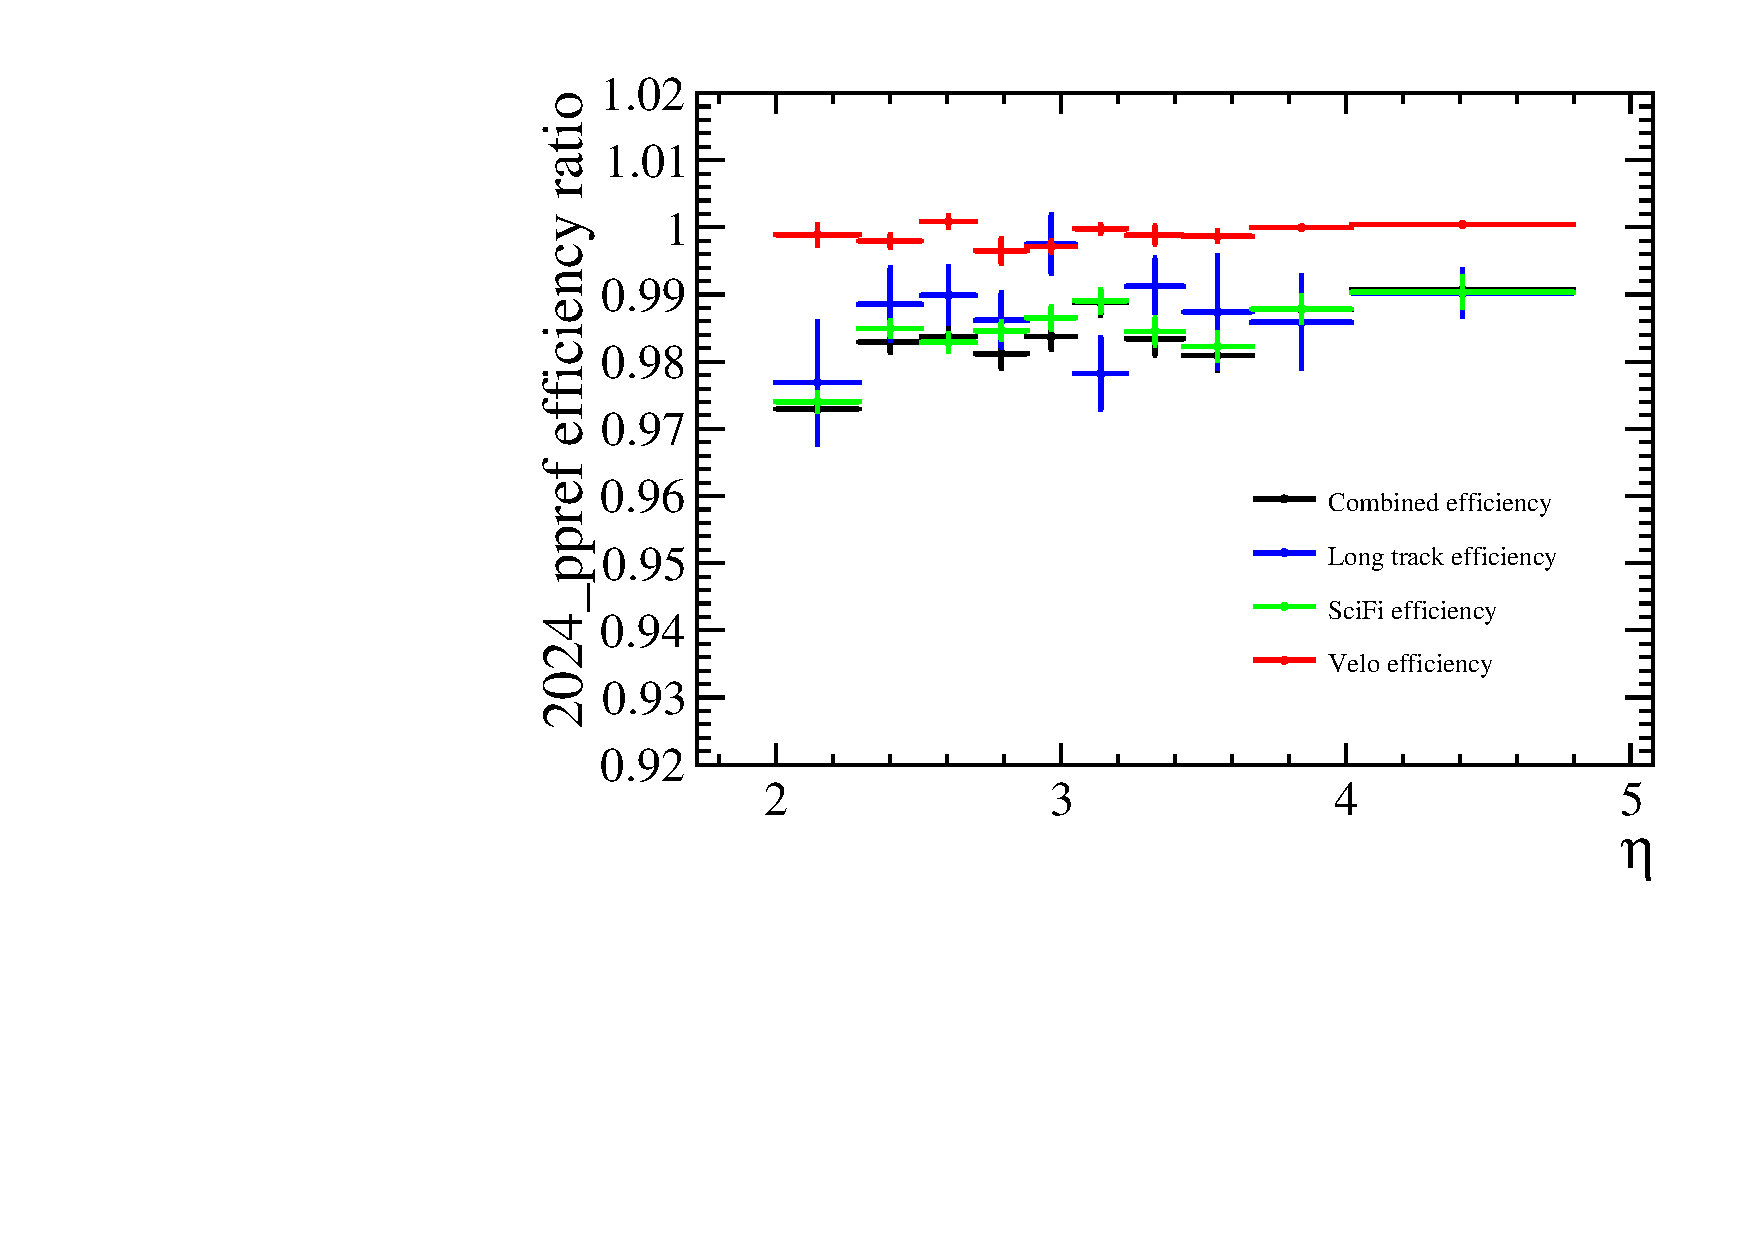
\includegraphics[width=1.0\textwidth]{Plots/trackeff_ratio_ETA_2024_ppref_default_samples.pdf}
    \end{subfigure}%
    \begin{subfigure}{0.5\textwidth}
      \centering
      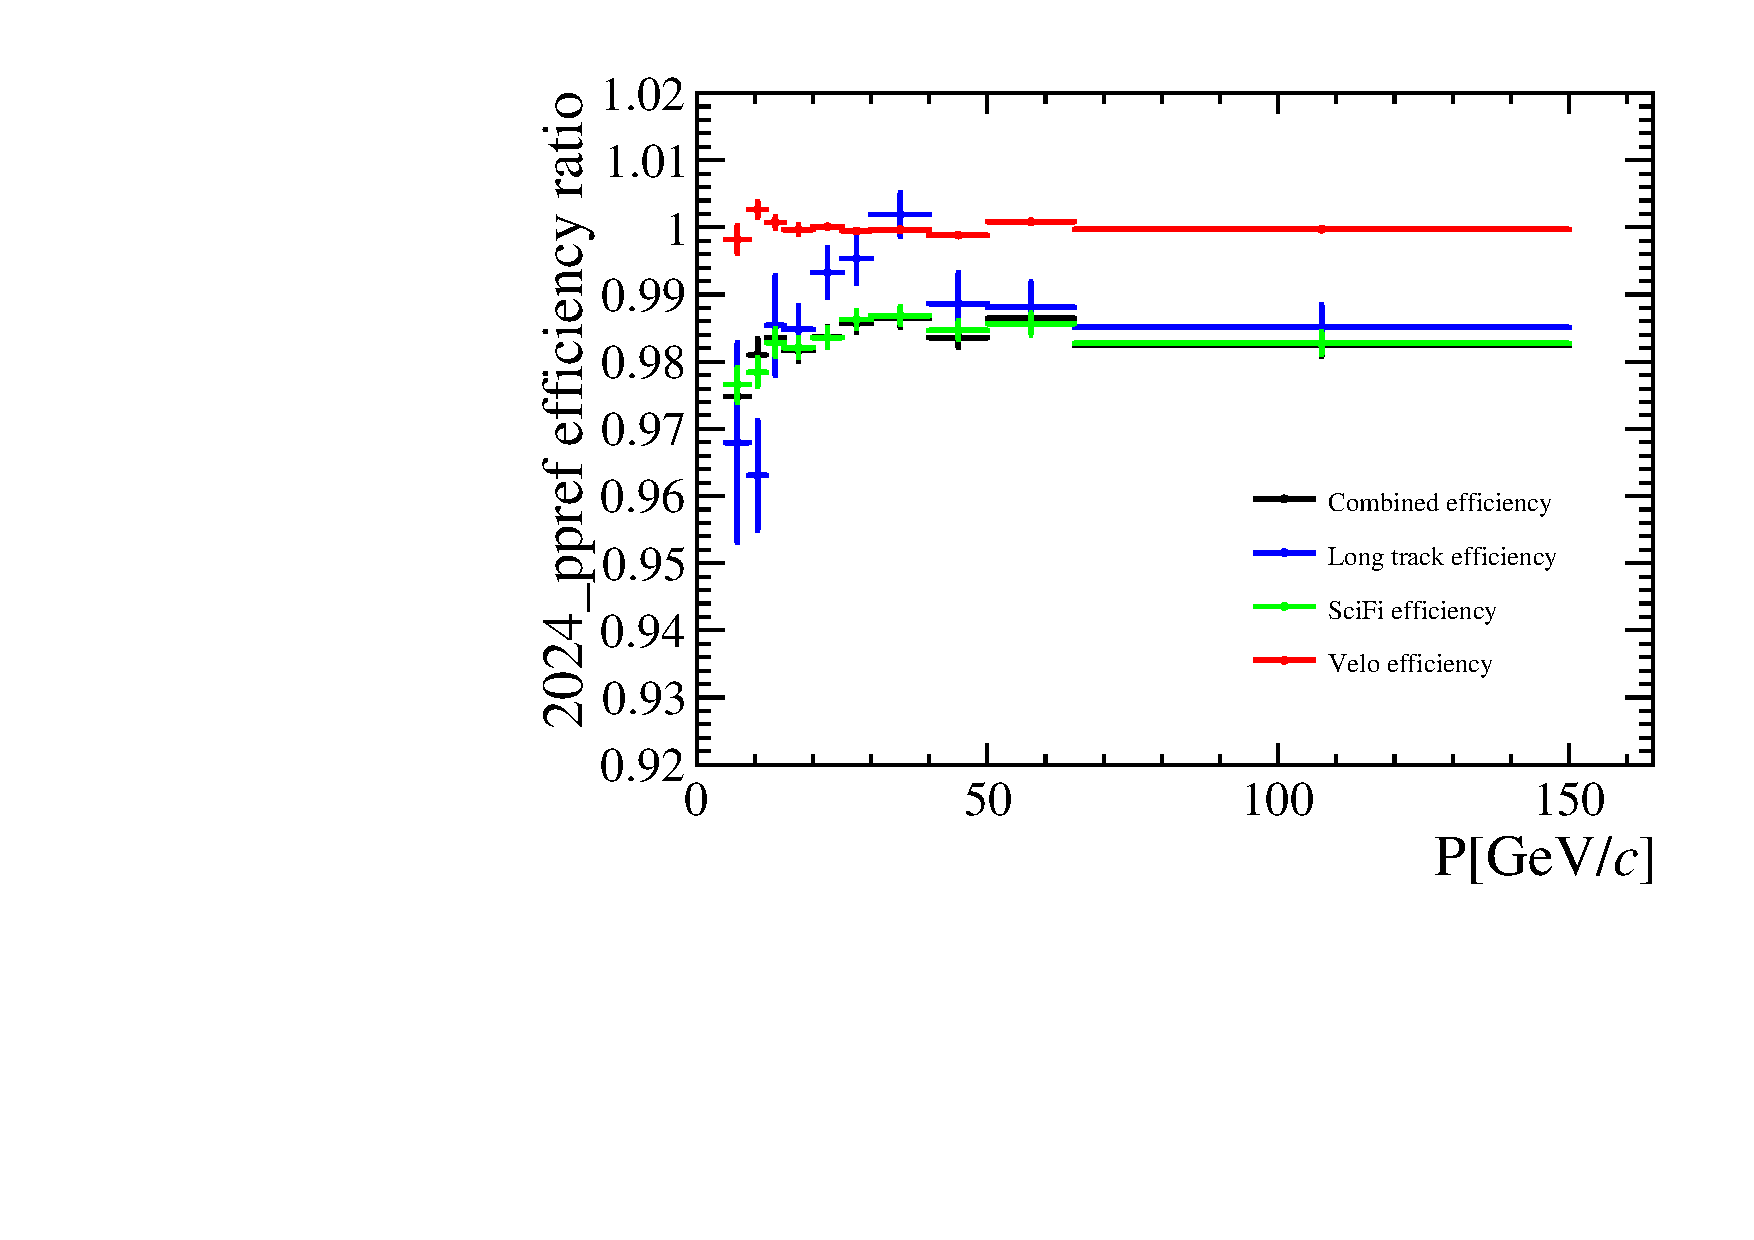
\includegraphics[width=1.0\textwidth]{Plots/trackeff_ratio_P_2024_ppref_default_samples.pdf}
    \end{subfigure}
  \end{figure}
  {Data/MC ratio for Combined/MuonUT track efficiencies $pp$ ref run}
\end{frame}

\begin{frame}{Tracking efficiency data/MC ratio}
  \vspace{0.0cm}
  {\large Data/MC ratio}
  \begin{figure}[htb]
    \centering
    \begin{subfigure}{0.5\textwidth}
      \centering
      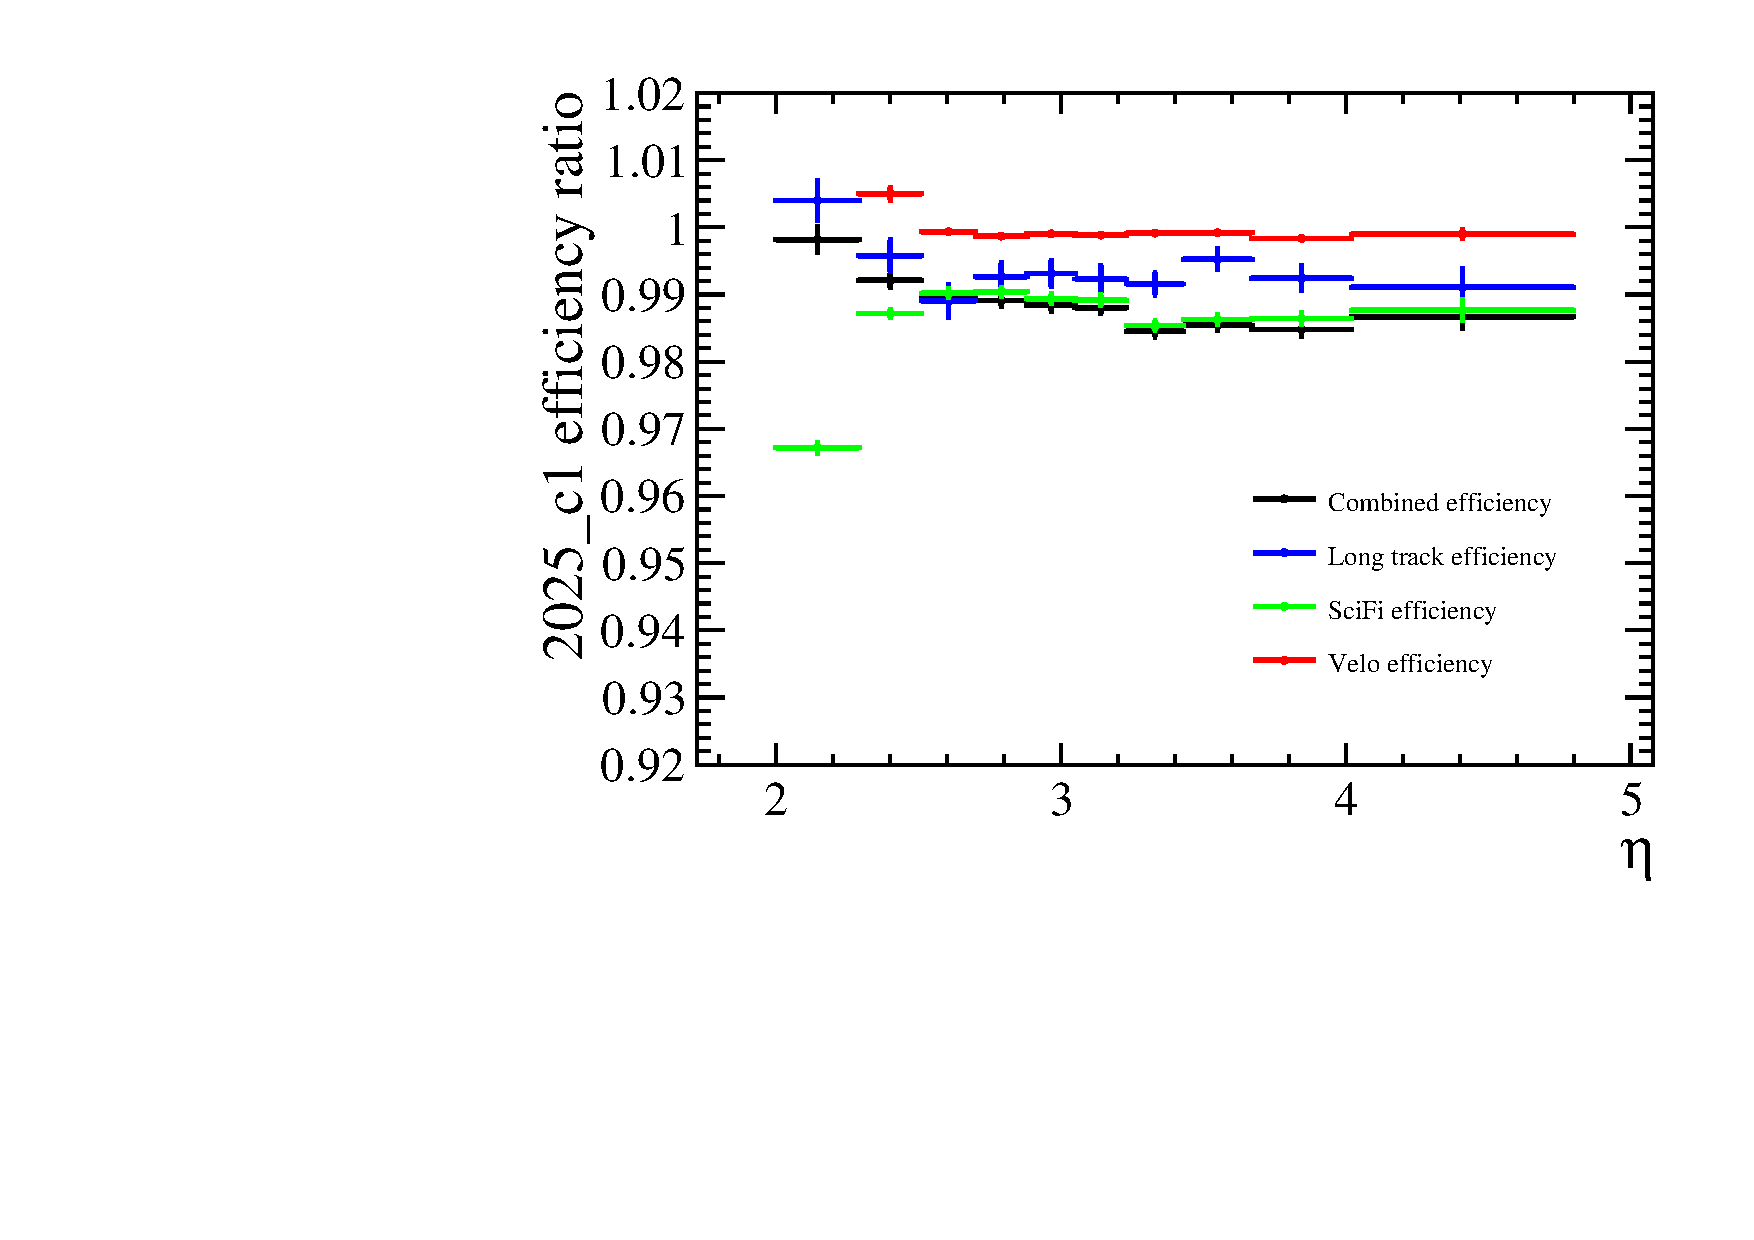
\includegraphics[width=1.0\textwidth]{Plots/trackeff_ratio_ETA_2025_c1_default_samples.pdf}
    \end{subfigure}%
    \begin{subfigure}{0.5\textwidth}
      \centering
      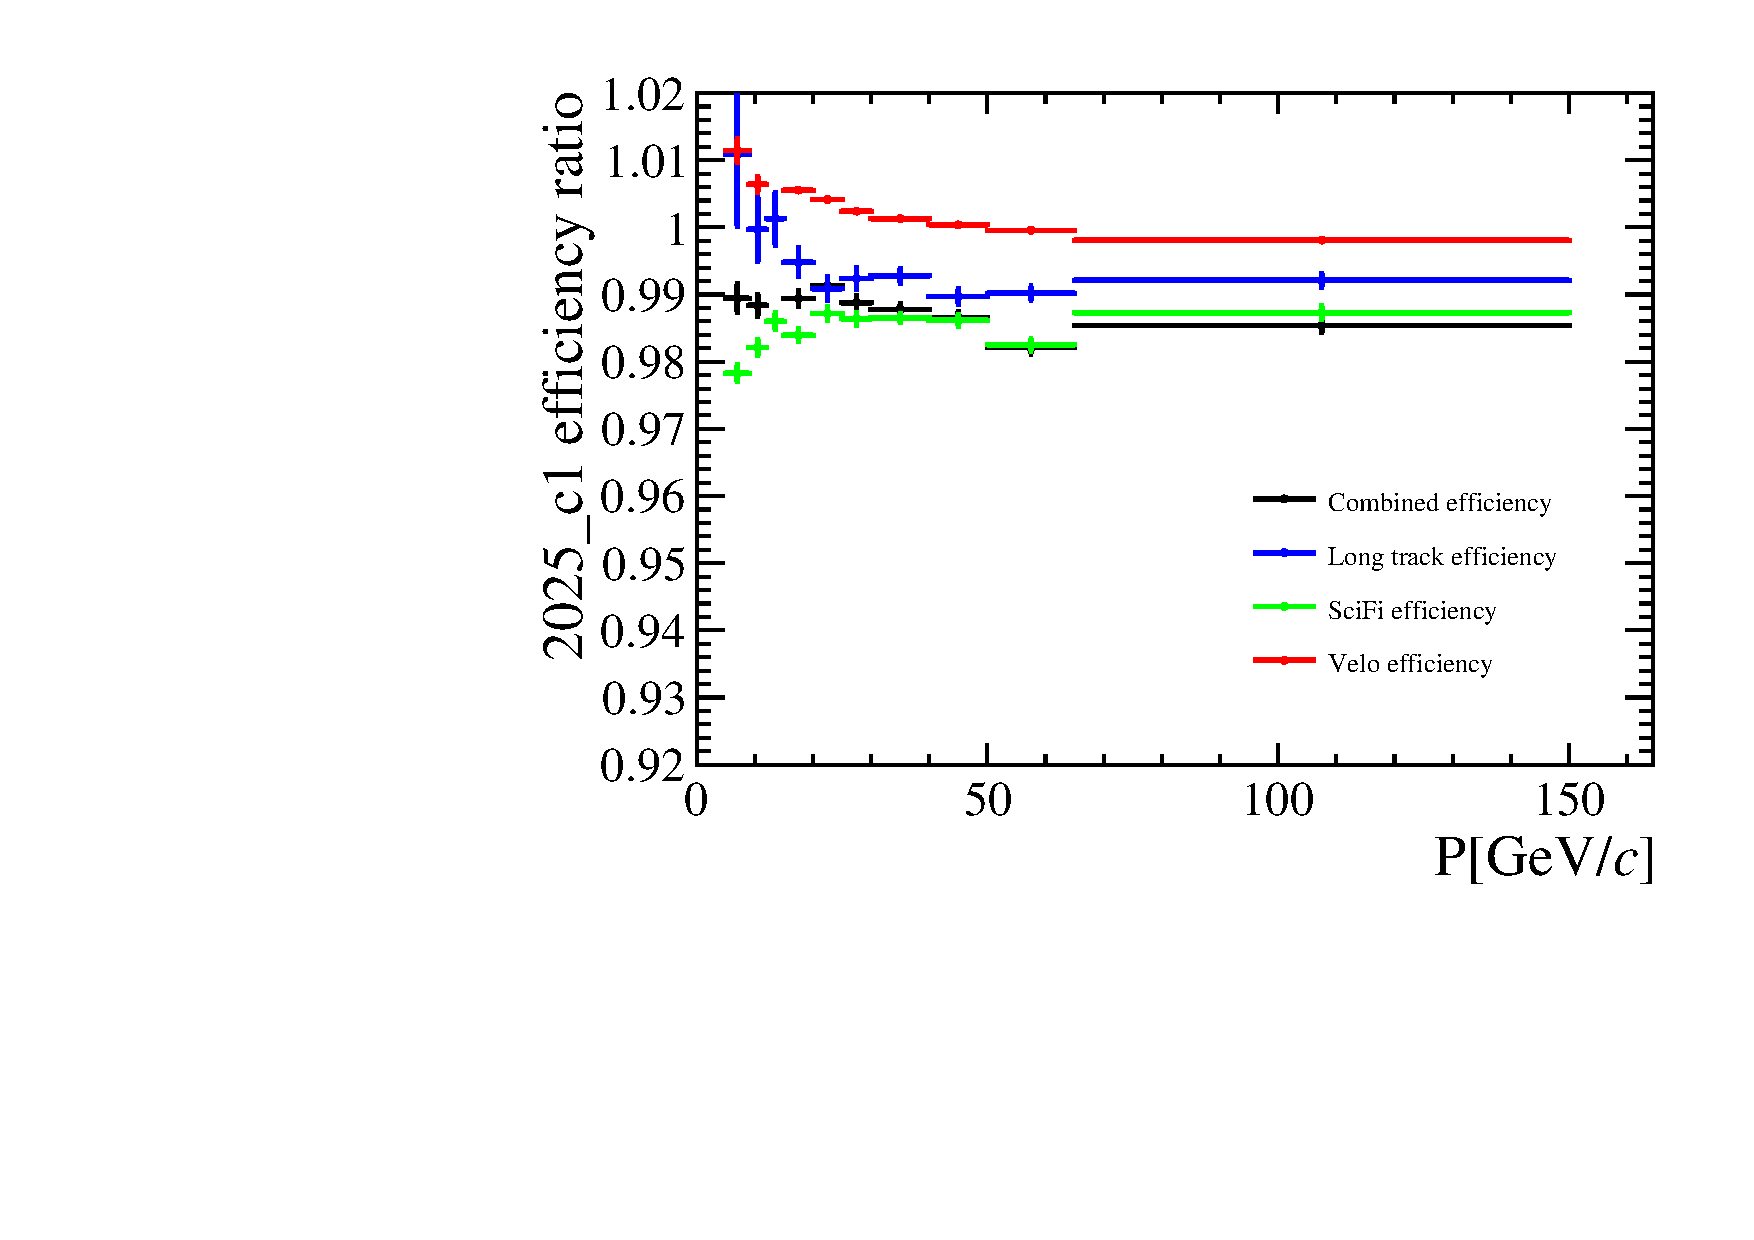
\includegraphics[width=1.0\textwidth]{Plots/trackeff_ratio_P_2025_c1_default_samples.pdf}
    \end{subfigure}
  \end{figure}
  {Data/MC ratio for Combined/MuonUT track efficiencies 2025 pre-TS}
\end{frame}

\begin{frame}{2D binning}
  \vspace{0.0cm}
  \begin{itemize}
    \setlength\itemsep{1.0em}
    \item{Currently we have 1D bins in $p$ and $\eta$ with 10 bins each}
    \item{Using $10\times10$ 2D bins is impossible}
    \begin{itemize}
      \setlength\itemsep{0.3em}
      \item{Insufficient statistics at high (low) $p$ and low (high) $\eta$}
      \item{But most bins \underline{do} have sufficient statistics}
    \end{itemize}
    \item{Strategy: Start with $10\times10$ bins and merge bins}
    \begin{itemize}
      \setlength\itemsep{0.3em}
      \item{Only consider MC, which is important for constraining the fit shape}
      \item{Only consider VeloMuon yields, as Downstream efficiencies are close to $100\%$ anyway and MuonUT is only used as a cross check}
      \item{Try to merge bins along $\eta$ at high $p$ and vice versa}
      \item{Aim for roughly $\gtrsim 100$ matched candidates in each bin}
    \end{itemize}
    \item{The next plots contain many (tiny) numbers, apologies for this!}
  \end{itemize}
\end{frame}

\begin{frame}{2D binning}
  \vspace{0.0cm}
  {\large Final 2D binning in $p$ vs $\eta$ with 72 bins:}
  \vspace{-0.4cm}
  \begin{figure}[htb]
    \centering
    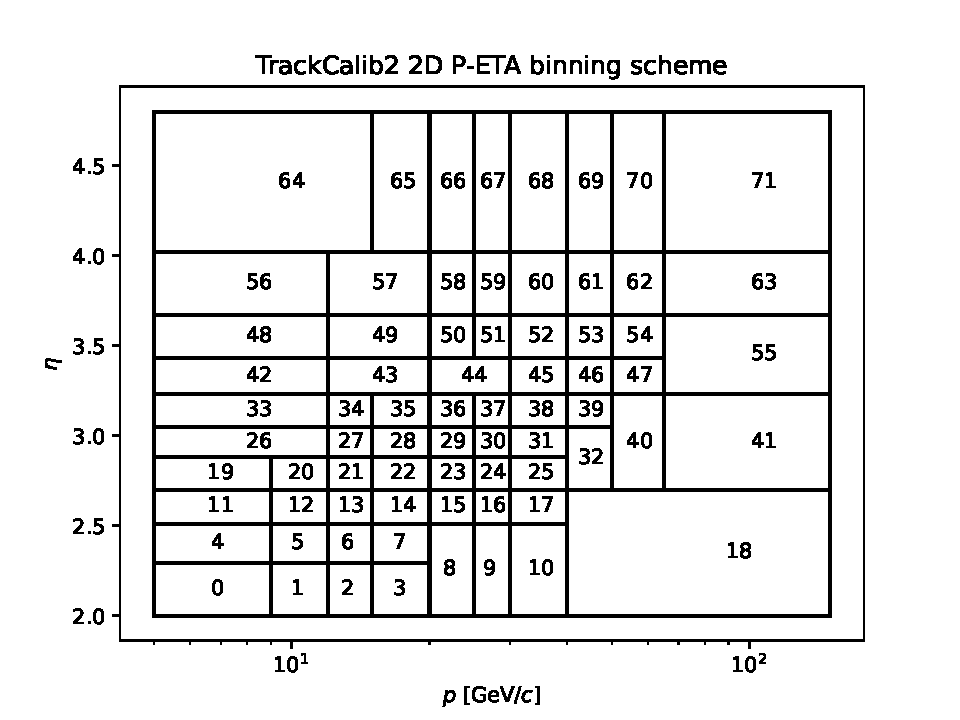
\includegraphics[width=0.8\textwidth]{Plots/TrackCalib2_2D_binning_scheme.pdf}
  \end{figure}
\end{frame}

\begin{frame}{2D binning}
  \vspace{0.0cm}
  {\footnotesize Combined result on top, long track result at the bottom}
  \vspace{-0.15cm}
  \begin{figure}[htb]
    \centering
    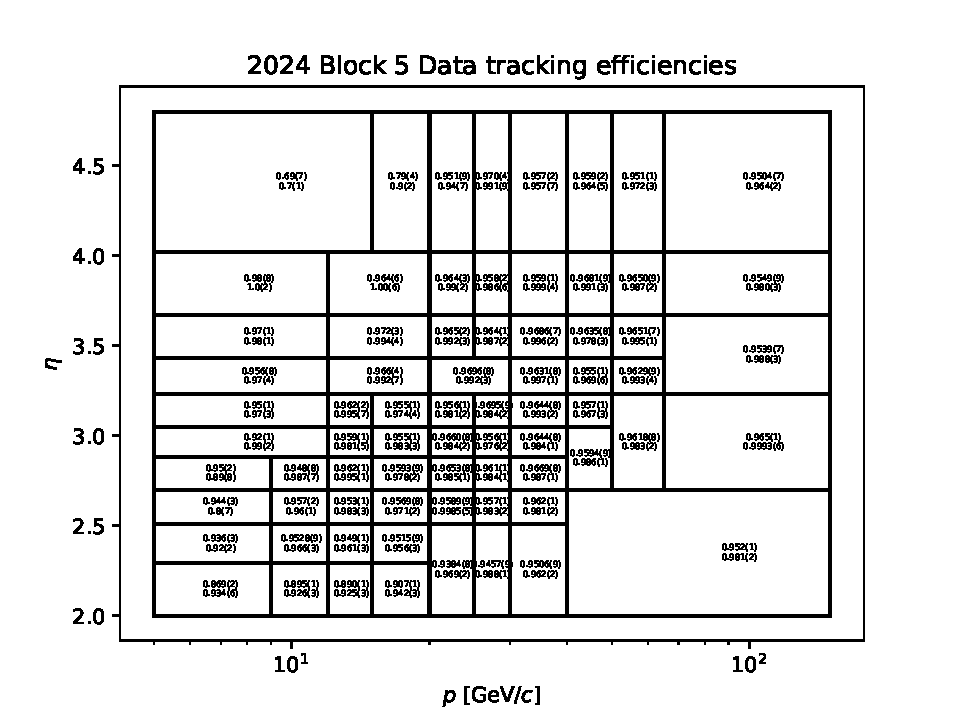
\includegraphics[width=0.85\textwidth]{Plots/TrackingEfficiencies_2D_binning_2024_Block5_Data.pdf}
  \end{figure}
\end{frame}

\begin{frame}{2D binning}
  \vspace{0.0cm}
  {\footnotesize Combined result on top, long track result at the bottom}
  \vspace{-0.15cm}
  \begin{figure}[htb]
    \centering
    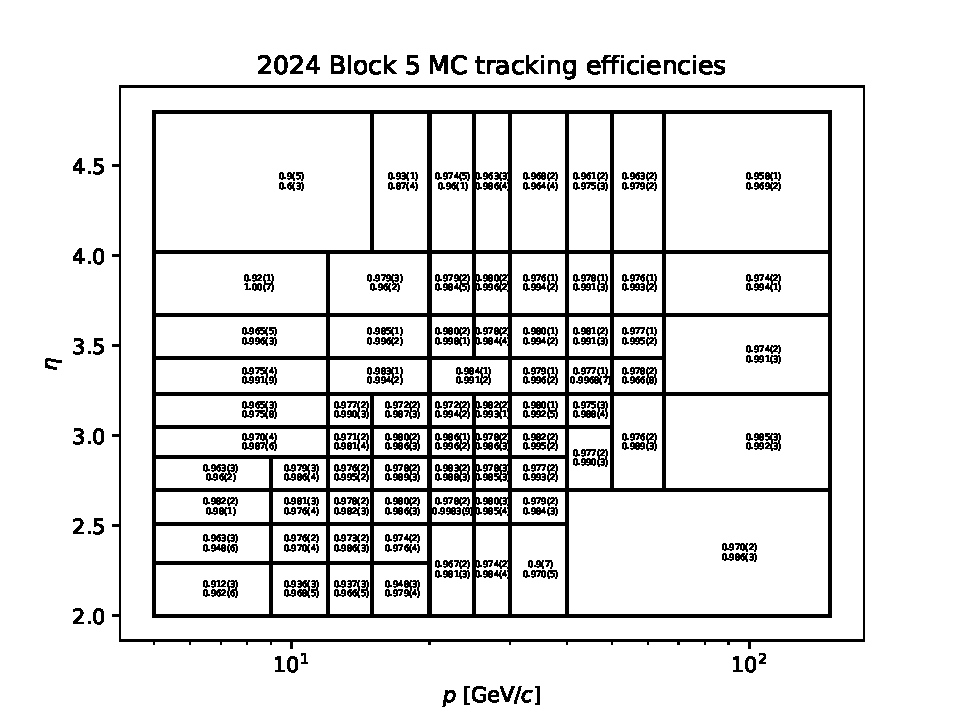
\includegraphics[width=0.85\textwidth]{Plots/TrackingEfficiencies_2D_binning_2024_Block5_MC.pdf}
  \end{figure}
\end{frame}

\begin{frame}{2D binning}
  \vspace{0.0cm}
  {\footnotesize Combined result on top, long track result at the bottom}
  \vspace{-0.15cm}
  \begin{figure}[htb]
    \centering
    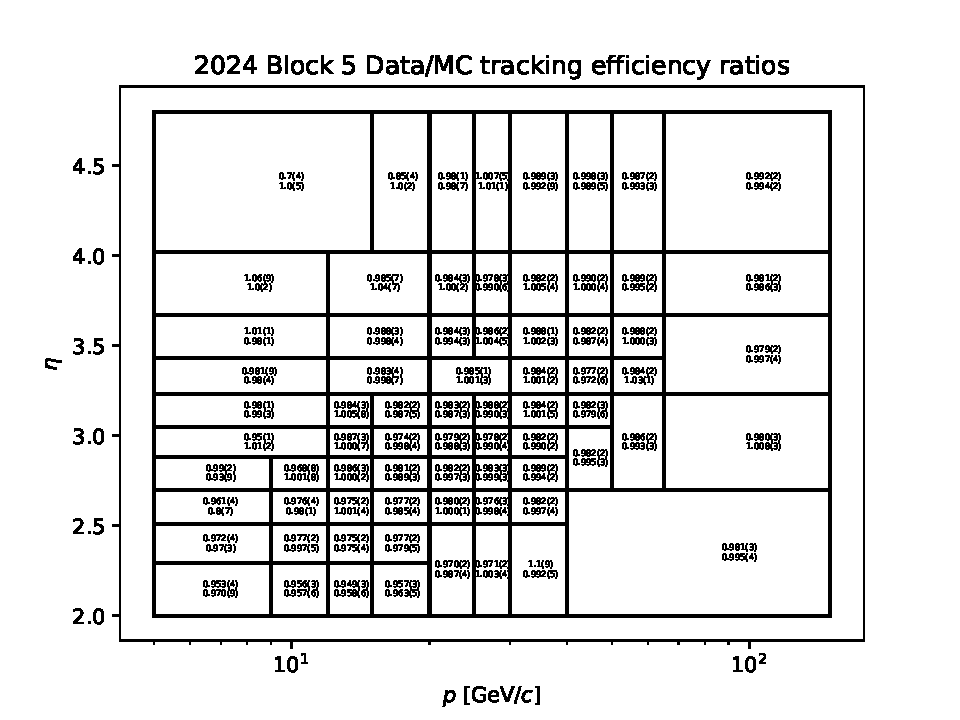
\includegraphics[width=0.85\textwidth]{Plots/TrackingEfficiencies_2D_binning_2024_Block5_Ratio.pdf}
  \end{figure}
\end{frame}

\begin{frame}{2D binning}
  \vspace{0.0cm}
  \phantom{\footnotesize Combined result on top, long track result at the bottom}
  \vspace{-0.15cm}
  \begin{figure}[htb]
    \centering
    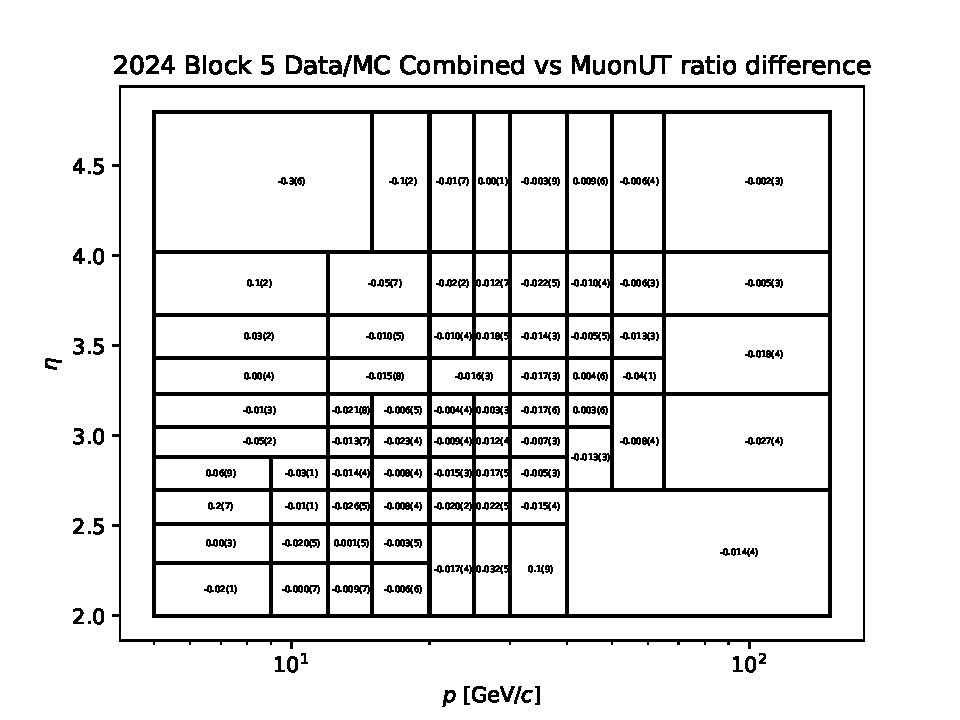
\includegraphics[width=0.85\textwidth]{Plots/TrackingEfficiencies_2D_binning_2024_Block5_RatioDiff.pdf}
  \end{figure}
\end{frame}

\begin{frame}{Combined vs MuonUT systematic}
  \vspace{0.0cm}
  {\large Combined vs MuonUT systematic strategy?}
  \begin{itemize}
    \setlength\itemsep{1.0em}
    \item{Clearly depends on kinematics, so we should use 2D binning}
    \item{It's a method systematic, should not depend on dataset with same $\mu$}
    \item{Our proposed strategy:}
    \begin{enumerate}
      \setlength\itemsep{0.5em}
      \item{Determine ratio difference for all data sets in each bin}
      \item{Combine blocks 5/6 and 7/8}
      \item{Use blocks 5/6 as proxy for blocks 1/2 due to bug in MuonUT trigger line (see \href{https://gitlab.cern.ch/lhcb/Rec/-/merge_requests/4047}{!4047} and \href{https://gitlab.cern.ch/lhcb/Rec/-/merge_requests/4050}{!4050})}
      \item{For bins with a discrepancy above $1\,\sigma$, assign the difference from zero as a systematic}
      \item{Systematic will most likely be small in most bins, but a small number of bins might have a $1\%$--$2\%$ systematic, in rare cases $> 3\%$}
    \end{enumerate}
  \end{itemize}
\end{frame}

\begin{frame}{Release of tracking efficiencies}
  \vspace{0.0cm}
  {\large We would like to do an initial release of 2024 tracking efficiencies}
  \begin{itemize}
    \setlength\itemsep{1.0em}
    \item{Binning schemes are defined in JSON files}
    \item{Tracking efficiencies in 1D and 2D bins also provided as JSON}
    \item{Data/MC ratio in 2D bins provided for physics analysis}
    \item{1D plots in $p$ and $\eta$ are also nice to release}
    \item{Initially release charge integrated numbers, but separate $\mu^+$ and $\mu^-$ results will follow}
    \item{Where would the most convenient location to put these files?}
  \end{itemize}
\end{frame}

\begin{frame}{Summary and next steps}
  \vspace{0.0cm}
  \begin{enumerate}
    \setlength\itemsep{1.0em}
    \item{Block 1b MC doesn't describe SciFi FE exclusion well}
    \item{Ready for initial release of 2024 blocks 2, 1a, 5--8, $pp$ ref}
    \begin{itemize}
      \item{Several issues have been resolved}
      \item{Behaviour consistent between blocks}
    \end{itemize}
    \item{2025 Velo efficiencies in MC need to be understood}
    \item{Additional work required for next release:}
    \begin{itemize}
      \item{Larger MC samples (maybe 4M $\to$ 10M), requires PPG permission}
      \item{Include \texttt{nFTClusters} reweighting using work by Maurice}
      \item{Other systematics}
    \end{itemize}
  \end{enumerate}
\end{frame}

\end{document}
